\documentclass[a4paper,12pt]{article}

\usepackage{comment}
\usepackage{supertabular}
\usepackage{graphics}
\usepackage{color,soul}
\usepackage{booktabs}
\usepackage{paralist}
\usepackage{algorithmicx}
\usepackage{algorithm}
\usepackage[noend]{algpseudocode}
\usepackage{booktabs}
\usepackage{hvfloat}
\usepackage{comment}
\usepackage{chngpage}
\usepackage{url}
\usepackage[utf8]{inputenc}
\usepackage[table,dvipsnames]{xcolor}
\usepackage[a4paper,pdftex,hmargin=0.75in,vmargin={1.1in,0.6in},head=75pt,foot=45pt, left=2.5cm, right=2.5cm, includefoot, footskip=60pt]{geometry}
\usepackage{lipsum}
\usepackage{afterpage}
\usepackage{xcolor}
\usepackage{tabularx}
\usepackage{wallpaper}
\usepackage{adjustbox}
\usepackage[normalem]{ulem}
\useunder{\uline}{\ul}{}
\usepackage{rotating}
\usepackage{parskip}
\usepackage{listings}
\lstset{language=C,breaklines=true}
\usepackage[english]{babel}
\usepackage{amsmath}
\usepackage{amsfonts}
\usepackage{amssymb}
\usepackage[justification=centering]{caption}
\usepackage{fontenc}
\usepackage[colorlinks=true]{hyperref}
\usepackage{multicol}
\usepackage{multirow}
\usepackage{array}
\usepackage{relsize}
\usepackage{subcaption}
\usepackage{caption}
\usepackage{tcolorbox}
\usepackage{lscape}
\usepackage{lastpage}
\usepackage{acro}
\setlength{\headsep}{1.5cm}
\usepackage[toc,page]{appendix}
\usepackage[nottoc]{tocbibind} % for show references in toc
\usepackage{pgfgantt}
\usepackage[gen]{eurosym}
\usepackage{xr}
\makeatletter
\newcommand*{\addFileDependency}[1]{% argument=file name and extension
  \typeout{(#1)}
  \@addtofilelist{#1}
  \IfFileExists{#1}{}{\typeout{No file #1.}}
}
\makeatother

\newcommand*{\myexternaldocument}[1]{%
    \externaldocument{#1}%
    \addFileDependency{#1.tex}%
    \addFileDependency{#1.aux}%
}
\usepackage[acronym]{glossaries}

\frenchspacing
%\usepackage{svg}
%\usepackage{showframe}% for show page layout

\colorlet{punct}{red!60!black}
\definecolor{background}{HTML}{EEEEEE}
\definecolor{delim}{RGB}{20,105,176}
\colorlet{numb}{magenta!60!black}
\lstdefinelanguage{json}{
    basicstyle=\normalfont\ttfamily,
    numbers=left,
    numberstyle=\scriptsize,
    stepnumber=1,
    numbersep=8pt,
    showstringspaces=false,
    breaklines=true,
    frame=lines,
    backgroundcolor=\color{background},
    literate=
     *{0}{{{\color{numb}0}}}{1}
      {1}{{{\color{numb}1}}}{1}
      {2}{{{\color{numb}2}}}{1}
      {3}{{{\color{numb}3}}}{1}
      {4}{{{\color{numb}4}}}{1}
      {5}{{{\color{numb}5}}}{1}
      {6}{{{\color{numb}6}}}{1}
      {7}{{{\color{numb}7}}}{1}
      {8}{{{\color{numb}8}}}{1}
      {9}{{{\color{numb}9}}}{1}
      {:}{{{\color{punct}{:}}}}{1}
      {,}{{{\color{punct}{,}}}}{1}
      {\{}{{{\color{delim}{\{}}}}{1}
      {\}}{{{\color{delim}{\}}}}}{1}
      {[}{{{\color{delim}{[}}}}{1}
      {]}{{{\color{delim}{]}}}}{1},
}

%RBG FFD33E / C95D40
\definecolor{upcorange}{HTML}{FFD33E}
\hypersetup{allcolors=black}

% probably a good idea for the nomenclature entries:
\acsetup{first-style=short}

%%%% PAGE STYLE %%%%%
\usepackage{fancyhdr}
\pagestyle{fancy}
\fancyhf{}
\lhead{
\includegraphics[height=1.2cm]{img/logos/upclogo.png}}
\rhead{
\includegraphics[height=1.2cm]{img/logos/logo_telecos.png}}
\rfoot{\thepage{}}

\renewcommand{\footrulewidth}{0.4pt}
%\futurelet\TMPfootrule\def\footrule{{\color{upcorange}\TMPfootrule}}
\futurelet\TMPfootrule\def\footrule{{\color{gray!80}\TMPfootrule}}
\renewcommand{\headrulewidth}{0.4pt}
\renewcommand{\headrule}{\hbox to\headwidth{%
%\color{upcorange}\leaders\hrule height \headrulewidth\hfill}}
\color{gray!80}\leaders\hrule height \headrulewidth\hfill}}
%\renewcommand*\ShowFrameColor{\color{red}}

% class `abbrev': abbreviations:
\DeclareAcronym{EU}{
  short = EU ,
  long  = European Union ,
  tag = abbrev % class
}

\DeclareAcronym{ETSETB}{
  short = ETSETB ,
  long  = Escola Tècnica Superior d'Enginyeria de Telecomunicació de Barcelona ,
  % long = Barcelona School of Telecommunications Engeneering ,
  tag = abbrev % class
}


\makeglossaries

\newglossaryentry{tip}{
name=tip,
description={The priority fee (tip) incentivizes validators to include a transaction in the block. Without tips, validators would find it economically viable to mine empty blocks, as they would receive the same block reward. Small tips give validators a minimal incentive to include a transaction. For transactions to be preferentially executed ahead of other transactions in the same block, a higher tip can be added to try to outbid competing transactions}
}

\newglossaryentry{gossip}{
name=Gossip protocol,
description={
The Gossip protocol is a protocol that allows designing highly efficient, secure and low latency distributed communication systems Peer-2-Peer(P2P)}
}

\newglossaryentry{economy-of-scale}{
name=economy of scale,
description={A proportionate saving in costs gained by an increased level of production}
}

\newglossaryentry{51-attack}{
name=51\% attack,
description={A 51\% attack is an attack on a distributed network by a group of dishonest nodes who control more than 50\% of the network's mining node rate. Owning 51\% of the nodes on the network theoretically gives the controlling parties the power to alter the state as desired
}
}

\newglossaryentry{json}{
name=JSON,
description={A JSON (JavaScript Object Notation) is a simple text formatting used for data communication}
}

\newglossaryentry{orm}{
name=ORM,
description={Object Relational Mapping (ORM) is a technique that creates a bridge between object-oriented programs and relational databases.}
}

\newglossaryentry{nonce}{
name=nonce,
description={A nonce is an arbitrary number used only once in a cryptographic communication created randomly or pseudo-randomly.}
}

\newglossaryentry{dom}{
name=dom,
description={The Document Object Model (DOM) is a programming interface for web documents. It represents the page so that programs can change the document structure, style, and content.}
}

\newglossaryentry{api}{
name=API,
description={API stands for application protocol interface, which is a set of definitions and protocols for building and integrating application software in other to communicate with other services and products without having to know how are they implemented.}
}


\newacronym{pow}{PoW}{Proof of Work}
\newacronym{pos}{PoS}{Proof of Stake}
\newacronym{evm}{EVM}{Ethereum Virtual Machine}
\newacronym{eth}{ETH}{Ether}
\newacronym{abi}{ABI}{Application Binary Interface}
\newacronym{ui}{UI}{User Interface}
\newacronym{ux}{UX}{User Experience}

\begin{document}

%%% COVER %%%
\fancypagestyle{alim}{\fancyhf{}\renewcommand{\headrulewidth}{0pt}
\cfoot{
\includegraphics[height=2.2cm]{img/logos/logo_telecos.png}}
}
\thispagestyle{empty}
\begin{center}
{\sffamily 
\resizebox{0.8\textwidth}{!}{
\includegraphics{img/logos/upc_completo+telecos.png}}\\
\vspace{1cm}
{\Huge Development of a DAPP}\\
\vspace{0.5cm}
{\color{black}\hrule height 1pt}
\vspace{1cm}
{\large{Master Thesis\\
submitted to the Faculty of the \\
Escola T\`ecnica d'Enginyeria de Telecomunicaci\'o de Barcelona \\
Universitat Polit\`ecnica de Catalunya \\
by\\
\vspace{0.4cm}
Gerard Castell Ferreres}}

\nocite{*} % only if you no use \cite{}

\vspace{1.5cm}

{In partial fulfillment\\
of the requirements for the master in\\
\textit{Advanced Telecommunication Technologies} \textbf{ENGINEERING}}

\vspace{2cm}

{{Advisor: Jose Luis Muñoz Tapia}} \\
{{Barcelona, October 20, 2023}}
\thispagestyle{alim}
}

%%% INDEX %%%
\end{center}
\newpage
\tableofcontents

%%% LISTS %%%
\newpage
\listoffigures
\listoftables

\printglossary[type=\acronymtype]

%%% REVISION %%%
\newpage
\section*{Revision history and approval record}

\selectlanguage{english}
\foreignlanguage{english}

\begin{center}
\tablefirsthead{}
\tablehead{}
\tabletail{}
\tablelasttail{}
\begin{supertabular}{|m{1.908cm}|m{2.398cm}|m{11.489cm}|}
\hline
\textbf{Revision} &
\textbf{Date} &
\textbf{Purpose}\\\hline
0 &
01/09/2023 &
Document \ creation\\\hline
1 &
18/10/2023 &
Document \ revision\\\hline

\end{supertabular}
\end{center}

\bigskip

{\selectlanguage{english}
DOCUMENT DISTRIBUTION LIST}

\begin{center}
\tablefirsthead{}
\tablehead{}
\tabletail{}
\tablelasttail{}
\begin{supertabular}{|m{8.205cm}|m{7.589cm}|}
\hline
\textbf{\ Name} &
\textbf{\ e-mail}\\\hline
\ Gerard Castell Ferreres &
gerardcastell97@gmail.com
\\\hline
Jose Luis Muñoz Tapia &
jose.munoz@entel.upc.edu
\\\hline

\end{supertabular}
\end{center}

\bigskip

\begin{center}
\tablefirsthead{}
\tablehead{}
\tabletail{}
\tablelasttail{}
\begin{supertabular}{|m{1.925cm}|m{6.1990004cm}|m{1.901cm}|m{5.6140003cm}|}
\hline
\multicolumn{2}{|m{8.324cm}|}{ Written by:} &
\multicolumn{2}{m{7.715cm}|}{ Reviewed and approved by:}\\\hline
 Date &
 01/09/2023 &
 Date &
 18/10/2023\\\hline
 Name &
 Gerard Castell Ferres &
 Name &
 Jose Luis \ Muñoz Tapia\\\hline
 Position &
 Project Author &
 Position &
 Project Supervisor\\\hline
\end{supertabular}
\end{center}


%%% ABSTRACT %%%
\clearpage
\newpage
\section*{Abstract}

{This thesis explores the development of a Decentralized Application (dapp). The fast growth of blockchain technology has provided an opportunity to revolutionize lots of industries by enhancing transparency, security, and accessibility. This research investigates the architectural design, implementation, and deployment of a dapp that leverages smart contracts to facilitate car insurance policy creation and management.

Key objectives include the development of a user-friendly interface for policyholders, where they can obtain policy proposals and when purchased ensure a secure, tamper-resistant policy ledger. The study assesses the technical and practical aspects of blockchain-based car insurance, emphasizing the advantages of decentralization in reducing fraud, optimizing administrative processes, and enhancing policyholder trust.

The findings highlight the potential of dapps to disrupt traditional insurance models, emphasizing their role in encouraging trust and transparency while streamlining policy management processes.}

\clearpage
\newpage
\section{Introduction}
{In today's highly digitized world, everyone and everything is connected and nearly every routine task we carry out relies on a piece of technology to be accomplished. Unfortunately, many of these processes are complex, have a lack of transparency or involve intermediaries which makes them slow and tedious. Companies and third parties have in their hands the governance of our information, which currently is the most powerful asset.}

{The Internet plays a crucial role in these interactions since it has become the main connectivity channel. However, it is characterized by a fundamental centralization of data, power, and control. Corporations have monopolized user data, platform access, and content distribution, raising concerns about privacy, censorship, and fairness. In response to these challenges, the next generation of the Internet, well-known as Web 3.0, along with decentralized applications (dapps) have emerged in order to offer a more decentralized, open, and user-centric digital experience.}

{The emergence of Web 3.0 and dapps represents a huge shift in the way we interact with and perceive the digital world. This transformation is driven by a combination of technological innovation, a growing desire for transparency and user control, and a fundamental rethinking of the traditional web's limitations, which opens up new possibilities for innovation, collaboration, and trust on the internet, redefining the way we engage with the digital world.}

\bigskip

\subsection{Statement of purpose}

{Given the emergence of dapps, this thesis aims to figure out how a traditional digital product can adapt its tech stack to harness the capabilities and advantages provided. The main objective is to develop and implement a decentralized application for a real case scenario in order to understand how it achieves to make apps user-centric and learn from the bowels which are the protocols and software that have evolved to implement such applications.}

\subsubsection{What dapps offer over usual web applications?}
Continuously, we need to interact with companies in a lot of scenarios such as checking where a delivery is in real-time, complaining about a service, canceling a purchase, making a reservation, and so on. For nearly all of those cases, we use their web application to carry out such communication. This way, the companies use their technology, such as web applications, to provide just the data that they want to their consumers. In this process, we should be concerned about two worrying topics:
\begin{enumerate}
    \item \textbf{Data Ownership.} The information exchanged between consumers and companies is often sensitive and personal. When we interact with these corporate web applications, we must consider the extent to which our personal data is collected, utilized, and potentially monetized by these companies. 
    \item \textbf{Centralized Control and Trust.} The centralization of technology platforms in the hands of companies introduces a reliance on trust. We entrust these entities with our data, often without direct insight into how it is managed and secured. Centralized systems are susceptible to data breaches or manipulation, which can leave consumers at a disadvantage.
\end{enumerate}

{Decentralized applications appear as an attempt to solve these issues. Dapps are software applications built over a decentralized network, usually blockchain technology such as smart contracts to automate and enforce rules within the application. Smart contracts are self-executing code that runs on a blockchain and automatically runs a set of predefined rules without the need for intermediaries. Thanks to these features, the dapps can address the data privacy and ownership problem:}

\begin{itemize}
    \item \textbf{User-controlled data.} Users are able to see the code that rules the smart contracts, what is to say, users can know what companies would be able to do before and after accepting the contract.
    \item \textbf{Blockchain security.} Data stored is cryptographically secured, making it really challenging for anyone to corrupt it. Hence, it ensures the integrity of user data.
    \item \textbf{Transparency.} The transparent nature of blockchain allows you to verify how your data is used. All data interactions, known as transactions, are recorded on the public ledger.
\end{itemize}

{Besides that, dapps take advantage of blockchain consensus philosophy to erase the centralized control and trust problem:}
\begin{itemize}
    \item \textbf{Decentralization.} Dapps operate on decentralized networks, typically based on blockchain technology. This decentralization means there is no central authority or intermediary that holds control over the application or your data. Trust is distributed across the network rather than being concentrated in a single entity.
    \item \textbf{Trustless Environment.} In a dapp, trust is not vested in a central authority. Instead, trust is established through the consensus mechanisms of the blockchain. Transactions are verified by a network of nodes, making it more challenging for any single entity to manipulate data or transactions.
    \item \textbf{Censorship Resistance.} Dapps are resistant to censorship, ensuring that access to the application remains open and uncontrolled. The code that contains a smart contract is accessible to everyone always and cannot be changed so companies cannot make unilateral decisions if the contract does not allow it.

\end{itemize}
{By releasing the management and ownership of data to the users, dapps provide a more user-centric, accessible, secure, and transparent model. They erase the need for trust in a single entity and instead share the trust across a network. Therefore, users leverage the power of Web 3.0, the power to own their data on the Internet.}

\subsubsection{Business case: Car insurance}
{Once the benefits of dapps are introduced, we may think about a huge amount of real scenarios where this technology could improve significantly the user experience. For this experiment, I have chosen a regular task that almost everyone has to do at least once in his life: contract car insurance.

The world of insurance has long been characterized by cumbersome policies, complex intermediaries, and, at times, a lack of transparency. However, the advent of blockchain technology has presented an opportunity to disrupt and revolutionize this industry, offering a new era of decentralized insurance applications. In this thesis, I explore the development and implications of a dapp designed for managing car insurance policies.

As we look into the idea of building this dapp, there are a lot of processes that can be automated and trusted in the smart contract such as policy cancellation with corresponding payment refund, claims processing with third parties or policy renewal. I will compare how these regular procedures are streamlined thanks to the dapp approach and how it leaves behind the traditional insurance model.

The motivation of this thesis is to highlight the contribution to the ongoing discourse about the transformation of the Internet through blockchain technology. By focusing on car insurance, an area with a wide audience, I aim to demonstrate the potential of dapps, not just as technological innovations but as a game changer for an industry that, for too long, has been defined by complexity, opaqueness, and a lack of understanding with intermediaries.}

\subsection{Requirements and specifications}

{In order to evaluate properly if the use of dapps truly can replace the current model I have developed an end-to-end scenario. To do so, the experiment requires the development of a frontend and a backend that shapes the whole dapp.

The frontend part consists of a web application in order to make the dapp accessible to the policyholders. This platform acts as a bridge to offer the users the features of the backend.

On the other side, the backend is divided into two parts. One consists of developing the smart contracts that are in charge of handling the policy business logic. In addition, I have developed a traditional backend server with a database to store all policy proposals before being purchased. 

This whole scenario runs locally on my computer through a tool that simulates the blockchain network. Therefore, smart contracts can be widely tested and executed without spending real money.

Although the whole experiment is developed on a standard laptop, there is a deep dive into the hardware requirements for deploying the dapp comparing the local and production scenarios in the appendix \ref{appendix:deployment-dapp}. 
}

\subsection{Work plan}

\subsubsection{Tasks and milestones}

{The development of this project has been divided into three stages: development of the smart contracts, development of the off-blockchain backend and database, and finally development of the frontend web application.}

 {The first step was to implement the smart contracts. To do so, I took a course about Ethereum, Solidity, and smart contracts development. Once I acquired the basis of these technologies, I was able to start coding the contracts for policy creation and management.
 At this point, the first milestone was achieved: Smart contracts were coded (\textit{Feature 1}) and I was able to deploy them locally and perform several operations:}
 \begin{itemize}
     \item The contracts were ready to receive transactions to create or cancel policies, which refunds instantly to the user.
      \item We could retrieve the policy data just with the company and the client accounts.
      \item We could report a claim as a client, and an external claim evaluator could approve or decline. If approved, it automatically pays the costs of the sinister.
      \item Policies can perform all actions while they are within the activation period. Once the end date arrives, the user has to pay the renewal to reactive the policy and continue enjoying the policy coverage.
 \end{itemize}
 
 {Once the smart contracts were developed, I took another course about how to build a backend server with a database. Afterward, I was able to develop the backend app that allowed me to generate the proposals that could be turned into policies on the blockchain:
 \begin{itemize}
     \item The app was able to, given car specifications and driver data, offer a bunch of coverage types with the associated pricing per month (\textit{Feature 2}).
     \item When the user wants to save a proposal with the selected coverage types it must be authenticated through his Ethereum address, this way, the proposals generated could be bound to the account and saved within the database (\textit{Feature 3}).
     \item Once the user purchases a proposal, the address of the policy smart contract generated can be sent to the backend to identify which proposals have been finally converted (\textit{Feature 4}).
 \end{itemize}
 
 {Eventually, I developed the frontend application, where I could combine the app interface with both, the backend and the smart contracts and give sense to the whole decentralized app. These were the features released:}
 \begin{itemize}
     \item The user deals with an interface where it can be logged with his Ethereum account (\textit{Feature 5}).
     \item The user can introduce his car specifications to obtain a list of coverage types with their price. He can select the desired configuration to include in the policy and generate a proposal (\textit{Feature 6}).
     \item The user can access a dashboard where he can see the stored proposals. The proposal view displays all data stored in the database and served through the backend. The user can purchase the policy through his wallet (\textit{Feature 7}).
     \item The user can access the dashboard with all policies purchased. At every policy page, all data is retrieved from the smart contracts. Users can cancel the policy and the proportional part of the premium paid (\textit{Feature 8}).
     \item The last feature, which I did not have enough time to finish, was to connect the renewal and claim features from the \acrshort{ui} app to the smart contract (\textit{Feature 9}).
 \end{itemize}

\subsubsection{Gantt Diagram}
\label{ssec:gantt}
\begin{figure}[H]
    \centering
    %\includegraphics[width=13cm]{img/diagram_gantt.png}
    \begin{ganttchart}[y unit title=0.4cm,
y unit chart=0.5cm,
vgrid,hgrid,
title height=1,
today=30,%
today offset=.5,%
today label=Now,%
bar/.style={draw,fill=cyan},
bar incomplete/.append style={fill=yellow!50},
bar height=0.7]{1}{30}

 % dies
 \gantttitle{Phases of the Project}{30} \\
 \gantttitle{2023}{30} \\
 \gantttitle{January}{3}
 \gantttitle{Feb.}{3}
 \gantttitle{March}{3}
 \gantttitle{April}{3}
 \gantttitle{May}{3}
 \gantttitle{June}{3}
 \gantttitle{July}{3}
 \gantttitle{August}{3}
 \gantttitle{Sept.}{3}
 \gantttitle{October}{3} \\
 
 % caixes elem0 .. elem9 
 \ganttgroup[inline=false]{Blockchain}{2}{5}\\
 \ganttbar[progress=100]{Training}{2}{3} \\
 \ganttbar[progress=100]{Feature 1}{4}{5} \\
 \ganttgroup[inline=false]{Backend}{6}{15}\\
 \ganttbar[progress=100]{Training}{6}{9} \\
 \ganttbar[progress=100]{Feature 2}{8}{11} \\
 \ganttbar[progress=100]{Feature 3}{12}{14} \\
 \ganttbar[progress=100]{Feature 4}{15}{15} \\
 \ganttgroup[inline=false]{Frontend}{16}{30}\\
 \ganttbar[progress=100]{Feature 5}{16}{18} \\
 \ganttbar[progress=100]{Feature 6}{19}{21} \\
 \ganttbar[progress=100]{Feature 7}{22}{25} \\
 \ganttbar[progress=100]{Feature 8}{26}{28} \\
 \ganttbar[progress=25]{Feature 9}{29}{30} \\

 
 % relacions
 \ganttlink{elem1}{elem2}
 \ganttlink{elem2}{elem3}
 \ganttlink{elem2}{elem8}
 \ganttlink{elem4}{elem5}
 \ganttlink{elem5}{elem6}
 \ganttlink{elem6}{elem7}
 \ganttlink{elem5}{elem10}
 \ganttlink{elem7}{elem11}
 \ganttlink{elem4}{elem9}
 \ganttlink{elem9}{elem11}
 \ganttlink{elem11}{elem12}
 \ganttlink{elem11}{elem13}


\end{ganttchart}

    \caption[Project's Gantt diagram]{\footnotesize{Gantt diagram of the project}}
    \label{fig:gantt}
\end{figure}

\bigskip
\subsubsection{Deviations from the initial plan}
There were two features that I did not have enough time to implement from the frontend web application even though the smart contracts were ready to be consumed:
\begin{itemize}
    \item The first one is the policy renewal. The renewal logic on the smart contracts was implemented in the first stage. However, there was not any backend logic implemented to propose a renewal premium taking into account the claims amount and the depreciation of the vehicle, which is a more realistic feature. Therefore, I consider it an incomplete feature without the backend part which I had no time to develop.
    \item The other one is the report of a claim. A sinister must have a third-party evaluator who qualifies the level of the incident and approves or declines the amount to refund. As I just have the client web app, I consider I would have to implement another app for the claim evaluators that also accesses the smart contracts and visualizes a list of claims. There, they can decide if the claim is approved or declined. This would be a great example of how smart contracts streamline communication with intermediaries since once the claim is approved, the smart contract immediately compensates the client with the appropriate amount which is implemented. Unfortunately, I consider developing this second web application requires too much extra time and the features cannot be closed.
\end{itemize}}

%%% StateOfTheArt %%%
\clearpage\section{State of the art of the technology used or applied in this thesis}
  

\subsection{Blockchain}
{A blockchain is a way of building a distributed ledger where the transactions that modify the ledger’s state are sequentially and immutably ordered by consensus. Therefore, Blockchain allows us to create a shared system to record what has happened. What has been recorded cannot be changed: it acts like a digital notary providing trust among parties. Note also that the information is shared because is built by different people, which is to say it is transparent and public. In addition, Blockchain technology, mainly the one based on smart contracts provides an extremely wide capability of programming our money.

In a blockchain, there are three main concepts: blocks, chains, and nodes. Block refers to data and state being stored in sequential groups of these blocks. To modify this state we have to perform a transaction of data, which needs to be added to a block to be finalized successfully. Furthermore, "chain" refers to each block referencing its parent. The data in each block cannot change without changing all subsequent blocks and would require the consensus of the whole network. Finally, the nodes refer to the computers which shape the network. They must agree upon each new block and the chain as a totality.

You can hear about a lot of benefits of using this technology such as data integrity, anonymity, reliability, etc. If we think about how it achieves all these properties we have to consider a combination of several ideas. Nodes are in charge of sharing the same state for everyone in the network. To achieve this, they negotiate through the consensus algorithm. }

\subsubsection{Source authentication, data integrity, and non-repudiation}
{We can start with how blockchain guarantees authentication and integrity. The public key cryptography plays a crucial role here. This algorithm is based on obtaining two keys, one public which is known by everybody and belongs to the user, and another private, which is known just by the owner. 

The private one is used to cipher a message, whereas the public one is used to decipher the message. This way, where someone decyphers the message with the public key it can verify that the message belongs to a certain owner since only he has the private key to do so, hence we get the \textbf{source authentication}.

Moreover, this data already signed cannot be modified, because I would need the private key to decipher and cypher again the message but the people just know the public key. So, just the private key owner can do this and we have achieved \textbf{data integrity} as well.

Note also that consequently, we are obtaining a very interesting property known as ``\textbf{non-repudiation}'', which merely refers to a situation where a statement's author cannot dispute its authorship.}

\subsubsection{One-way hash functions}
{Once we know how to protect data we have to think about the blockchain network. The objective of this network is to store data. This data can only be modified through transactions. Somehow, we are talking about a database. There is a basic requirement for a database which is a fast search capability. To achieve a great performance, it is applied one-way hash functions to the inputs, so the outputs are used as keys of the database. To decrease the capacity of that two different inputs generate a collision, i.e. generate the same hash, we are going to use really huge output space with 256 bits. Therefore, thanks to ``one-way hash functions'', given a hash output, it is computationally unfeasible to find the input.
More details about hashing are explained more deeply in appendix \ref{appendix:hashing}}.
\begin{figure}[H]
\centering
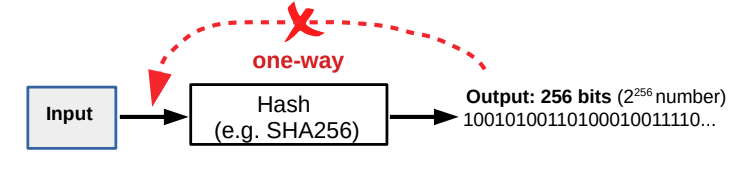
\includegraphics[width=12cm]{img/chapter_2/one-way-hash-functions.png}
\caption[One way functions]{\footnotesize{One way functions.}}
\label{fig:one-way-functions}
\end{figure}

\subsubsection{Transactions and consensus}
{Most of the ledgers that we usually use are centralized. All data is stored in a single computer and that makes it simple and it could be fast or convenient for an end user too. However, centralization has a drawback to consider: the power is centralized as well, and that is a risk if you cannot trust the owner. Banks are the typical example of this, but blockchain is attempting to offer a better solution. To do so, it relies on distributed systems, which are models in which components located on networked computers, \textbf{nodes}, communicate and coordinate their actions by passing messages. They have separated memories consolidating a shared state, where the ledger can be stored.

Now we are able to introduce how the ledger handles money. Users of the blockchain can create money movements, called \textbf{transactions}. All transactions are authenticated by their owners, even though we need \textbf{consensus}. The consensus is in charge of providing an order. This is fundamental in a ledger with the aim of avoiding negative balances. In a distributed system the consensus plays a main role since it has to ensure that the network avoids stuck states, stops if it is asynchronous, and progresses when the network recovers. Note that this means to force determinism, so external sources can just be injected as a transaction.

Another interesting property of money is to keep anonymity. Bank transfers are directly bound to the implied persons, whilst pocket money is not, so current digital transactions are not keeping this property. Blockchain pursues to resolve this too by creating an account ID that cannot be linked to a person. Users create a pair of public and private keys, sometimes the address is a derivation of the public key, and use that to sign the transactions on the network. Hence, everyone can have more than one account, and public keys have absolutely not any relation to the person's ID. 

Every blockchain has a different way of achieving consensus, in the case of Ethereum was accomplished initially thanks to \acrfull{pow} which was introduced by Bitcoin. Nevertheless, due to several reasons, Ethereum eventually migrated to \acrfull{pos} in 2022, which nowadays is a more common alternative and is increasing in popularity.

Both \acrlong{pow} and \acrlong{pos} are complex algorithms that are explained thoroughly in appendices \ref{appendix:proof-of-work} and \ref{appendix:proof-of-stake} respectively. It is a recommended reading in order to understand better the sense of consensus. 
}

\subsubsection{Cryptocurrencies}
{A cryptocurrency is an asset to exchange secured and trusted by a blockchain ledger. It represents a medium of exchange that is accepted as payment for goods and services. Blockchain allows users to make transactions over the network that would remain registered in the ledger without needing a third party to maintain them.

These cryptocurrencies are what the miners receive in compensation for the effort of mining new blocks and behaving honestly in the blockchain. This is the usual way the blockchain creates more tokens.

The first cryptocurrency was Bitcoin, created by Satoshi Nakamoto\cite{sathoshi}. Nowadays, thousands of blockchains and cryptocurrencies have appeared and evolved from Bitcoin.  }

\subsubsection{Wallets} \label{section:wallets}
{If a blockchain aims to process payments, every user will expect some software or hardware to interact with the network. Since there are many non-trivial concepts to take into account when interacting with the network, such a technology has to fit several requirements, some of which are the following: }
\begin{itemize}
    \item Show account balance, even in different currencies and blockchains.
    \item Manage multiple accounts.
    \item Manage user private keys: generate, backup, and so on.
    \item Send transactions and display transactions history.
\end{itemize}

{This item is what a \textbf{wallet} does.

Since wallets can manage a handful of accounts, and each one has its key pairs, they end up with a simple idea: Remember a single secret, which is the master, and derive all the key pairs from it. These types of wallets are called \textbf{Hierarchical Deterministic Wallets} \cite{hd-wallet}, or HD wallets. 

HD wallets ensure that all addresses needed are generated from a single seed instead of being randomly generated on demand, as you may see in figure \ref{fig:hierarchical-deterministic-wallet}. The seed is expressed in the form of a twelve-word seed-word phrase called \textbf{mnemonic}. Different public keys of the same HD wallet cannot be correlated unless you know the seed.}

\begin{figure}[H]
\centering
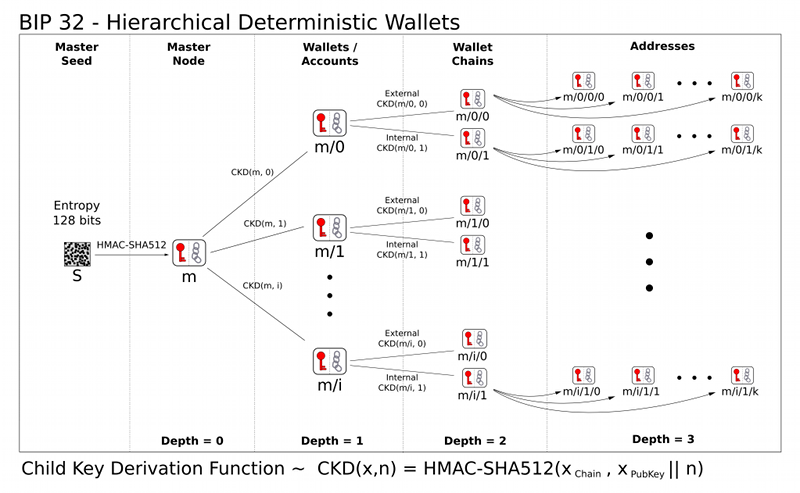
\includegraphics[width=14cm]{img/chapter_2/hierarchical-deterministic-wallet.png}
\caption[Hierarchical deterministic wallet]{\footnotesize{Hierarchical deterministic wallet.}}
\label{fig:hierarchical-deterministic-wallet}
\end{figure}

{One of the most popular software wallets is Metamask \cite{metamask}. Metamask is an HD wallet built as a browser extension that provides access to blockchain networks. When a user installs Metamask, it generates a random mnemonic and prompts the user to save it. Then, Metamask asks the user to introduce a password that will be used to encrypt the master secret and store it in the browser's local storage, which is known as \textit{vault}.


\begin{figure}[H]
\centering
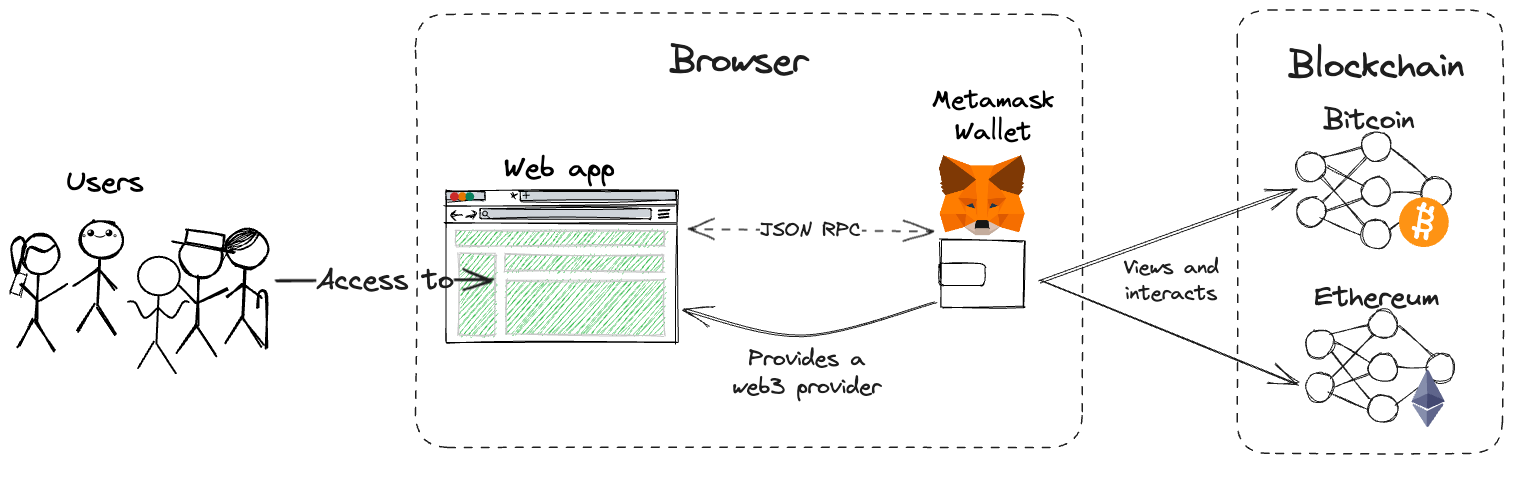
\includegraphics[width=14cm]{img/chapter_2/metamask-provider.png}
\caption[Metamask as web3 provider]{\footnotesize{Metamask as web3 provider.}}
\label{fig:metamask-mnemonic}
\end{figure}

As is illustrated in figure \ref{fig:metamask-mnemonic}, Metamask is designed to be a browser wallet. Wallets act as \textbf{web3 provider} to connect the different blockchains. The analogy is to think about this web3 provider as a telecom company offering you access to the cell network. Without such a provider, web applications would not be able to access the blockchains. This communication is carried out through the JSON-RPC protocol.}

\bigskip

\myexternaldocument{blockchain}
\subsection{Ethereum}
{
Ethereum motivation was to leverage the first blockchain networks, such as Bitcoin, and overcome their constraints. In a nutshell, Ethereum is a blockchain that works like a computer embedded, so is prepared to run apps and organizations in a decentralized, permissionless and censorship-resistant way.

In Ethereum, we can talk about a single computer called \acrfull{evm} that establishes which is the state that every node on the network should agree on. Any participant can broadcast a request for \acrshort{evm} to perform a computation over the state. When it happens, other participants on the network validate and ensure the request is signed by the address that sends it. If verified, then they check if that address has permission to execute the state change, if so they do it. Consequently, the state changes in the EVM and propagates throughout the network. Such requests for computations are called transaction requests and are stored on the blockchain by order along with the current state of the \acrshort{evm}. 

A "node" is any instance of Ethereum client software that is connected to other computers also running Ethereum software, creating a network. To read more information about the Ethereum client you can find it in appendix \ref{appendix:ethereum-client}.

Ethereum gathers a lot of concepts and the core ones are explained in the following sections. For more information, you can start by reading the original {Ethereum Whitepaper}\cite{ethereum-whitepaper}.
}

\subsubsection{Ethers}
{\acrfull{eth} is the native cryptocurrency of Ethereum and its purpose is to boost a market for computation. \acrshort{eth} represents an economic incentive for participants to provide computational resources to the network, which allows transactions to be validated and executed.

In Ethereum, when users want to make a transaction, they must pay some amount of \acrshort{eth} to the network as a bounty. These usage costs are known as gas fees. The network will award to the participant that eventually verifies the transaction, executes it and commits it to the blockchain.

This ``\gls{tip}" that senders pay, is equivalent to the amount required by the resources to carry out the computation and depends on the demand of computation power at that moment. Furthermore, paying an amount also prevents malicious participants from blocking the network by requesting infinite computation or other intensive tasks since they must pay for computation resources. If a task runs out of all the ether fees paid, the transaction gets terminated and the network returns to normal.

\acrlong{eth} can just be created on the creation of a new block process and is performed by the protocol definition, so any user can create. About 1/8 of the total issuance goes to the block proposer, whilst the remainder is distributed across the other validators. By contrast, \acrlong{eth} is destroyed on every transaction. This process is called ``burning'' and the removal is permanent. When users pay for their transactions a base gas fee is destroyed. This amount is defined by the blockchain according to the computation power demand.

The \acrshort{evm} stores the state, and this state is a ledger of all the accounts that have executed a transaction on the network. The final state provides us the current balance in \acrshort{eth} of all the accounts. Such accounts are able to send, hold and receive \acrshort{eth} from other accounts and interact with deployed smart contracts. We may find two types of accounts:
\begin{itemize}
    \item Externally-owned accounts (EOA), controlled by a person with the private key.
    \item Contract account, which is a smart contract deployed to the network and controlled by the code.
\end{itemize}
}

\subsubsection{Gas}
{Gas refers to the unit that measures the amount of computational effort required to execute specific operations on the Ethereum network. Each transaction to the network requires computation resources to execute. Such resources must be paid for to ensure Ethereum cannot get stuck in infinite computational loops. Note that regardless the transaction fails or succeeds the computation could have been carried out so the fee is paid in any case. Therefore, this gas fee appears to justify the payment for computation as is reflected in figure \ref{fig:gas-per-computation}.

\begin{figure}[H]
\centering
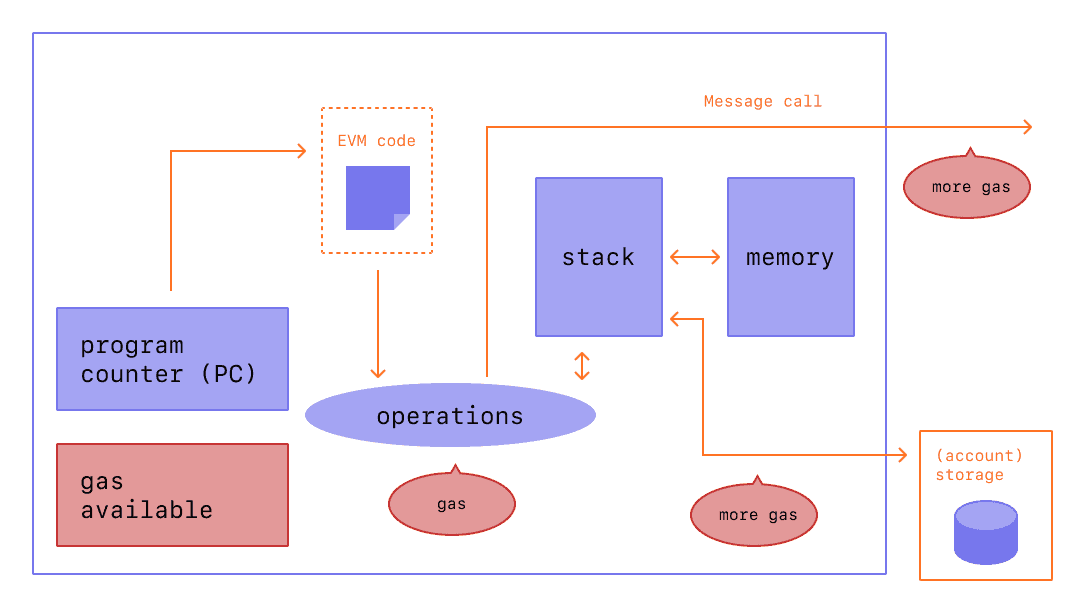
\includegraphics[width=12cm]{img/ethereum/gas.png}
\caption[Gas consumed per computation]{\footnotesize{Gas consumed per computation.}}
\label{fig:gas-per-computation}
\end{figure}

If we want to calculate the gas fee that a transaction requires we have to define it as the amount of gas used to do some operation, multiplied by the cost per unit gas. The \acrshort{evm} specifies the units of gas required by each computational operation \cite{opcodes-evm}. On the one hand, the base fee is set by the protocol depending on the number of blocks before it so it is easily predictable for users. On the other hand, the priority fee incentivizes validators to include a transaction on the block. The minimum amount of gas to pay is the base fee, but without a tip validators most likely will choose other transactions over yours or even create blocks with no transactions since they would receive the same award. So it is important to make this gas estimation predictable so users that offer too much waste some \acrshort{eth} or, by contrast, users that offer too little will not get a validator that chooses the transaction.  

Gas fees have to be paid in \acrshort{eth} and it is divided in two components: the \textbf{base fee} and the \textbf{priority fee} or \gls{tip}.


It is important to mention that users can define the maximum limit they are willing to pay for their transactions. This parameter is known as \textit{maxFeePerGas} and it must be greater than the sum of the base fee and the tip. The transaction sender is refunded with the difference between the max fee and the sum of the base fee and tip. This parameter is crucial because gas fees can get so high due to too much computation power demand or even complex smart contracts apps doing lots of operations.
}
\begin{figure}[H]
\centering
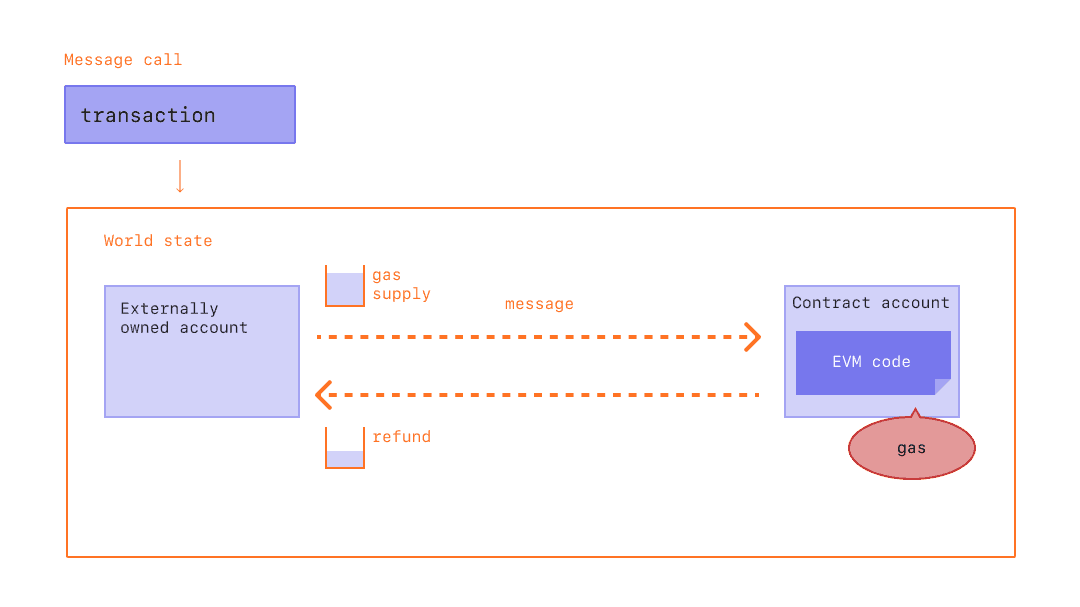
\includegraphics[width=12cm]{img/ethereum/gas-tx.png}
\caption[Gas refund procedure]{\footnotesize{Gas refund procedure.}}
\label{fig:gas-tx}
\end{figure}

{In brief, gas fees help to keep the Ethereum network secure. By requiring these bounties for computation it prevents bad actors from clogging the network. In addition, it also helps to avoid accidental loops or other intensive computational wastage in code.}


\subsubsection{Ethereum Virtual Machine (EVM)}
{The \acrlong{evm} is present at any block in the Ethereum's chain and it is in charge of defining the rules for computing a new valid state from block to block.

Ethereum is in essence a \textbf{distributed state machine}, in which state is a large database that holds not only all accounts and their respective balances but also a state machine. This state machine can execute arbitrary machine code and change between blocks according to a pre-defined set of rules defined by the \acrshort{evm}.

The state data structure that contains the large database is called a \textit{modified Merkle Patricia Trie}, which points to all addresses by hashes based on a single root hash such as the Merkle tree idea explained thoroughly in appendix \ref{appendix:merkle-tree}. This system lets to verify transactions in the network really fast and without the need for knowing all the content.

Ethereum is like a \textbf{state transition function} where given an input, the \acrshort{evm} returns a deterministic output. In terms of state, the expression would be \(Y(S, T)=S'\), where \textit{S} is a valid old state, \(T\) a handful of new valid transactions, \(Y(S, T)\) is the transition function and \(S'\) is the new valid state. 

Transactions are instructions from accounts signed beforehand which can be classified into two types: \textbf{message calls} and \textbf{contract creation}. The last type results in the creation of a new contract account containing compiled smart contract bytecode. Whenever a message call is addressed to this contract account the bytecode is executed.


\acrshort{evm} contains several pieces as you may see in figure \ref{fig:ethereum-node}. One of them is a \textbf{memory} which lives during execution by is no persisted between transactions. Nevertheless, contracts contain also a Merkle Patricia \textbf{storage} associated with the contract account as part of the global state. 

\begin{figure}[H]
\centering
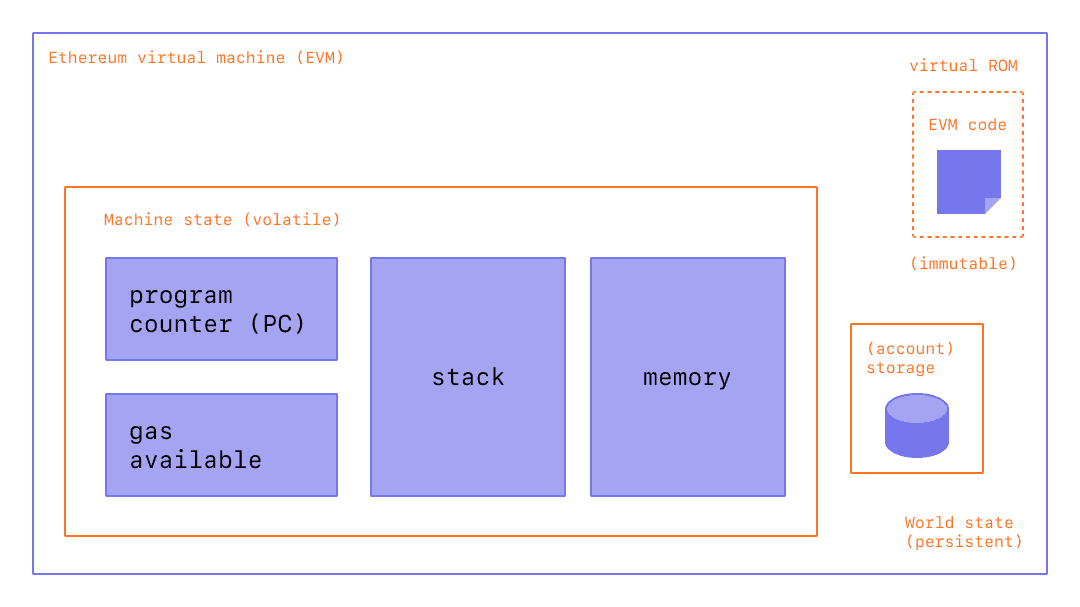
\includegraphics[width=12cm]{img/ethereum/evm.png}
\caption[Diagram of EVM internal components]{\footnotesize{Diagram of EVM internal components.}}
\label{fig:ethereum-node}
\end{figure}

Compiled smart contracts can perform standard stack operations such as {\small\textit{XOR, AND, ADD or SUB}}. In addition, \acrshort{evm} also implements some operations for blockchain purposes like {\small \textit{ADDRESS, BALANCE, BLOCKHASH}}, etc.

}

\subsubsection{Smart Contract}
{At this point, the power and potential of Ethereum is quite clear. The capability to add executable code within the state machine streamlines many recurrent tasks to the extent that developers no longer need to write new code each time they want to request a computation to the \acrshort{evm}. Instead, they can upload programs into the \acrshort{evm} state and make a request to them in order to execute those lines of code which may be configurable with varying parameters of the call. Those scripts uploaded and executed by the network are smart contracts.

One of the most explained analogies about a smart contract is a vendor machine. In a vendor machine, if you introduce correct inputs (money and snack selection), a certain output is guaranteed (snack is dispensed).

Deploying smart contracts is public. To do so, we just need to code a smart contract with some Ethereum developer language such as Solidity, the one chosen for this experiment. Such languages are compiled before being deployed so the \acrshort{evm} can understand the bytecode. Moreover, we need some \acrshort{eth} since deploy means to request a transaction, so we have to pay gas fees.

It is important to highlight a big constraint. They cannot get information about real-world events because the state machine needs to be deterministic and such events are happening off-blockchain. If we inject external data in the middle of a computation it will pollute security and decentralization so determinism could not be achieved. Likewise, using such external data really enhances the scope and value of smart contracts. So to solve it, data is introduced and stored in the blockchain by what is known as \textbf{oracles}. Once the data is recorded on the blockchain it can be consumed by smart contracts, but cannot be changed which ensures determinism is achieved.

In a nutshell, smart contracts are simply programs that run on the Ethereum blockchain. They can perform a set of actions, their functions, and handle data, their state, that is located to an Ethereum address, hence they have a balance and can receive and send transactions to any other address. This allows to call of other smart contracts that encourage composability.
}


\subsubsection{Decentralized Applications (dapps)}
{
What really empowers Web 3.0 are the decentralized applications. To define what is a decentralized application, we need to gather all the aforementioned concepts. A dapp is an application built on a decentralized network that combines smart contracts and a frontend user interface. Ethereum defines every smart contract as public, meaning transparent and accessible, hence any frontend application can interact with any smart contract, acting as an open \Gls{api}, even if you are not the owner of the smart contract.

If we think about how standard apps are implemented, we may define two isolated domains: frontend and backend. In the case of a dapp, the backend code runs on a decentralized peer-to-peer network like a blockchain instead of a centralized server. About the frontend, it could be written in any code like the apps do. If we focus on the hosting, the backend code is also hosted in the blockchain, whilst the frontend is not required, so it can be served from any centralized server. In practice, developers use web libraries such as ``\textit{ethers.js}"\cite{ethers} which will trigger and interact with the browser wallets like \textbf{Metamask}. Such wallets use \textbf{JSON RPC} protocol to connect through a public node, such as ``\textit{infura}"\cite{infura} or \textit{``geth"}\cite{geth}, to Ethereum and therefore, to the smart contract. This tech stack illustrated in figure \ref{fig:ethereum-node} is what conforms to a decentralized application.
}

\begin{figure}[H]
\centering
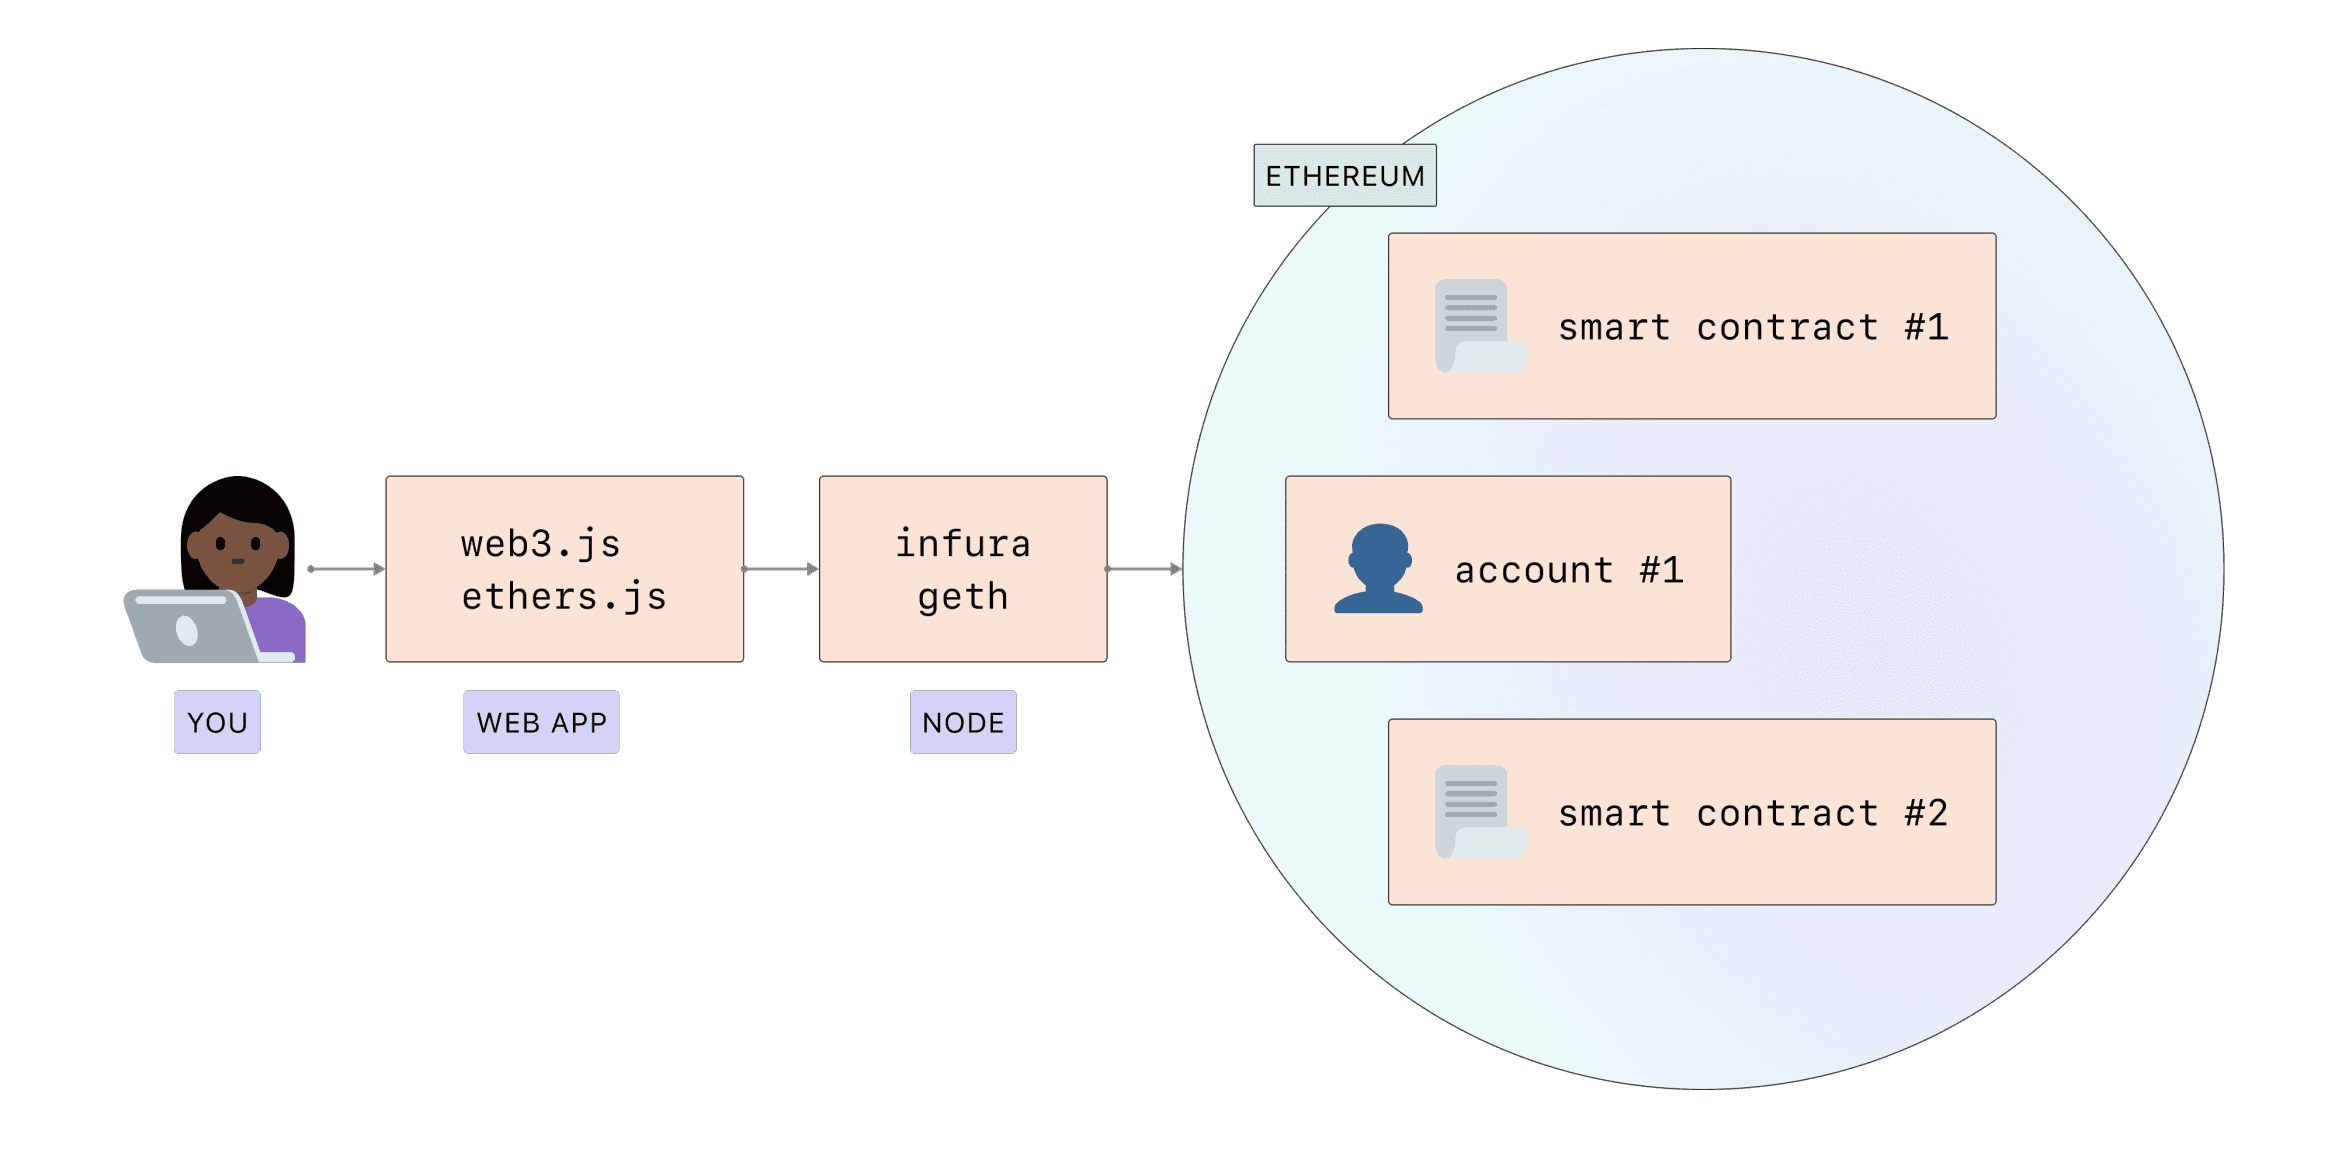
\includegraphics[width=14cm]{img/ethereum/nodes.png}
\caption[Ethereum connection from web applications]{\footnotesize{Ethereum connection from web applications}}
\label{fig:ethereum-node}
\end{figure}

{Dapps rely on their business logic in the network through the smart contracts, which run computations on the \acrlong{evm}. Such a code is always deterministic, meaning that given the same network state and the same input transaction, it is going to return the same output. It is also important to note that what is sent to the network cannot be changed so we must be very careful about the code that we write. It has bugs such as infinite loops or exhaustive processes that waste so much gas or even in the worst case security glitches, we could be able to update the code to fix them, so they must be designed and tested thoroughly. Opting for dapps provides some interesting benefits over usual applications but also has drawbacks that we must take into account. 

On the one hand, one of the most important advantages is the \textbf{zero downtime}. Since the code is deployed as a smart contract on the blockchain, the network will always be able to serve client requests so the service is never suspended. The blockchain wrapping also offers more \textbf{privacy} because the users will use address accounts to interact that are not linked to persons. In addition, dapps ensure \textbf{data integrity} on the blockchain. Such data is immutable and malicious actors cannot corrupt persisted information. Eventually, the more significant game changer properties are \textbf{censorship resistance} and 
\textbf{trustless behavior}. Smart contracts can be analyzed and predict what they will compute and return in a deterministic way, which completely replaces the need for trust in third parties with opaque processes. Moreover, no single entity can unilaterally block users from submitting transactions to change or read the state. This does not mean that we cannot define rules that allow just certain accounts to perform some actions but it must be coded in the moment of deployment. 

On the other hand, we may find some disadvantages to take into account, starting with \textbf{maintenance}, which requires complex solutions since we cannot modify the code once deployed. There is also a huge \textbf{performance overhead} because Ethereum demands that every node runs and stores each transaction and, in addition, \acrlong{pos} takes its time as well. Furthermore, there is a possibility of the network getting congested since it can only process 10-15 transactions per second, if the rate of transactions is greater than the capacity to process them or the computation required increases the mempools will be full of unconfirmed transactions. Eventually, if we take a look at the user experience consuming the dapp it can be penalized as well. Most end-users might find it difficult to understand the Ethereum basis and use this kind of tools that really leverages blockchain power. In favor of reducing this effect, software solutions built on top of the base layer of Ethereum might end up trusting part of the logic and data managed in centralized services which could eliminate partially the benefits of blockchain.

There is more detail about the Web evolution until the Web 3.0 model in the appendix \ref{appendix:web-evolution}.
}


%%% METHODOLOGY %%%
\clearpage\section{Project development }
{In order to develop the insurance dapp, the process is divided into two parts as explained previously: backend and frontend.}

\subsection{Backend partition}
{For the backend, we will talk about the cohabitation of a traditional centralized backend app with smart contracts on the blockchain. This is due to the business model selected for the experiment. In an effort to represent a realistic scenario we have to note that all data stored in the blockchain will suppose a transaction, hence it will consume \acrshort{eth}, i.e. money. This raises the first decision of the project: select which data have to be stored on the blockchain in order to not exclude all its benefits. When thinking about insurance, we have to keep in mind a mental model about the flow a user carries out in order to contract a policy in the off-blockchain model: }
\begin{enumerate}
\label{enumerate:insurance-flow}
    \item User accesses a web platform where he is asked for his car specifications.
    \item Such information is sent to the backend as a ``{quote}". The backend executes some computations to generate pricing according to the risk assumed.
    \item Backend returns to frontend app a policy proposal that includes the coverage types available and their respective price per month.
    \item The web app displays the pricing by coverage, so the user may decide if the price convinces him and select which coverage types to include in his proposal. If the proposal is attractive for the user he can save it in the backend.
    \item Once the user decides to purchase the proposal, he introduces his credit card and confirms. Then, the payment proceeds at the backend, usually along with third-party entities that are specialists in bank interactions. If the whole process succeeds, the policy is bound to the user in a centralized database. The backend notifies the frontend that the process has been terminated successfully.
    \item The frontend notifies the user as well and for the rest of the ``life of the policy" the user will interact with the company through the web app to modify or read data from his policy. We will consider a couple of actions that a user can perform with an active policy:
    \begin{itemize}
        \item Make a claim: The user suffers a sinister which is covered by his policy so he uses the web app to report it and claim a refund for the possible damages. The backend receives the claim and the claim evaluator analyzes the details. If proceeds, the evaluator notifies the insurance company, which pays the third-party payment intermediary to refund the client or externals involved. Otherwise, if the claim is declined the company notifies the user through the app directly and no refund is carried out.
        \item Cancel the policy: The user decides to finish the policy unilaterally. The company gets notified and then it has to notify the third-party intermediary to refund the client.
    \end{itemize}
    \item If the end date of the policy arrives and the user has not canceled, the policy turns inactive and no operation can be performed to modify the state. The company offers a renewal proposal or not to the user with a new price taking into account depreciation and claims occurred. If the user accepts we go back to the first point.
\end{enumerate}

{
We may identify a main entity in the process which is the \textbf{policy}. The policy is what defines the contract with the user so it would collect all the data related to what the user has paid, what has been insured and which action could perform. We can make the analogy of a user purchasing the proposal with a transaction to the smart contract because in both processes we are paying and amount to execute a computation. This computation results in storing the policy with its corresponding data. 

Nevertheless, there is a previous process where the user is still not paying and requires computation, which is the \textbf{quote}. When the user quotes in the traditional model, the backend is computing an estimated price to assume the risk. If we translate this model to the blockchain world, we would have to pay for every possible quote. In terms of economics, this is absolutely not profitable since we do not know yet if the user will eventually purchase the policy. So even in the best scenario where the user confirms, we would have to increase the price considering a rough fee based on the quote per purchase ratio. If we observe usual businesses this purchase rate per price discovered, equivalent to a quote, is usually quite low. Therefore I have decided to avoid this computation on blockchain.

With the aim of overcoming this quote computation constraint, I designed a mixed on-blockchain/off-blockchain solution that relies on the quote computation and storage of the backend logic into a centralized server, whilst the policy management and storage keep in the smart contract in favor of blockchain advantages. Henceforth, we will consider centralized backend as \textbf{off-blockchain} and smart contract backend \textbf{on-blockchain}.
}

\subsection{On-blockchain backend}
{
I started developing the smart contract because it is in charge of managing the policy entity which is the core of the business case. To develop the smart contract I chose Solidity\cite{solidity} as one of the most popular languages for writing smart contracts. 

The code written with Solidity is compiled to generate at least two files: an \acrfull{abi} and a Bytecode. The bytecode is the compiled code of the smart contract at low-level and readable by the \acrshort{evm}, whilst the \acrshort{abi} is a \Gls{json} file that describes the smart contract functions and data structures and how to interact with them. Such \acrshort{abi} is going to be crucial for the frontend part so after deploying it, the web must be able to access this file in order to be able to prepare the transactions according to the smart contract's expected input. To read more about how is the smart contract code you will find more information in the appendix \ref{appendix:smart-contract}.
}
\subsubsection{Policy smart contract}
\label{section:policy-smart-contract}
{

Regarding the car insurance flow commented at \ref{enumerate:insurance-flow}, the policy smart contract is in charge of storing the data. To create this smart contract we need to collect the following data:
\begin{itemize}
    \item \textit{riskData}. A JSON object with the specific details of the drive and car covered.
    \item \textit{premium}. The total amount of \acrshort{eth} paid by the user for the insurance service.
    \item \textit{owner}. The account address of the owner of the policy, which references the user.
    \item \textit{factoryAddress}. Sets the factory smart contract address. This value is not pre-defined for security reasons. We have to be able to propose new versions of the contracts.
    \item \textit{renewalDate}. The date the user defines as the end date of the policy. On that date a renewal
\end{itemize}

Besides this data, there are some more properties that are settled on contract deployment. The first one is the \textit{endDate}, which initially is equivalent to the renewal date. It will remain the same unless the user or company cancels the policy before the renewal date for some justified reason. The other property is the \textit{startDate} to consider the policy effective, which is set to the block timestamp of the \acrshort{evm} that computes the operation. Eventually, it also stores an empty array of \textit{claims}.

If we think about the functions we can group them into three types depending on the purpose. One of the more interesting is the \textit{modifiers}. They look after to meet certain conditions and if not they terminate the transaction. These functions are used by other functions to check conditions before executing their code. An example from the experiment is a modifier that checks whether the sender of a transaction corresponds to the address of the insurance company. Then, the function \textbf{renew}, which renovates the policy, can just be executed by the insurance company address. Furthermore, there is also another modifier that ensures the transaction sender is the owner of the policy which is the client and it is used in the method to make claims. There are four modifiers in this smart contract:
\begin{itemize}
    \item \textit{onlyOwner}. A modifier to check if the sender is the owner of the policy.
    \item \textit{onlyFactory}. A modifier to check if the sender is the factory smart contract.
    \item \textit{onlyFactoryOrOwner}. Combining the previous two we obtain another one that ensures the send is either the owner or the insurance address.
    \item \textit{isActive}. A modifier that ensures the policy end date is future to the execution time so it checks the policy to be active.
\end{itemize}

In addition, there are a handful of functions that are simple \textit{getters} to retrieve the data of the contract. These getters are really useful for the web application to consume and display the information in a more understandable and fancy way. All the getters of the contract are protected with modifiers that ensure the data can just be called by the insurance company or the owner.

The remaining functions are the ones that perform the computations to modify the state. A brief explanation about then:
\begin{itemize}
    \item \textit{cancelPolicy}. It can just be executed if the policy is activated and sets the \textit{endDate} to the block timestamp.
    \item \textit{makeClaim}. It can be called by the owner if the policy is active. Adds a new claim data structure to the list.
    \item \textit{approveClaim}. It can be called by the factory. Look for the claim in the list and set the expenses of the sinister. Then calls \textit{resolveClaim} accepting the refund.
    \item \textit{declineClaim}. It can be called by the factory. Calls \textit{resolveClaim} declining the refund.
    \item \textit{resolveClaim}. It is a private method. It stores on the claim the block timestamp and if it is accepted or declined.
    \item \textit{renew}. It can just be executed by the factory. Updates the \textit{endDate}, \textit{renewalDate} and \textit{premium} to the values suggested by the company and executed by the client.
\end{itemize}

Note that some of the functions do not make sense without the Factory contract explained in the section \ref{section:factory-sc}.

The entire code of this smart contract may be found in the appendix \ref{appendix:policy-sc}.
}

\subsubsection{Factory smart contract}
\label{section:factory-sc}
{
Once the policy smart contract is defined we have translated the policy management on the blockchain. Nevertheless, the objective of the dapp is to offer a real car insurance service and to achieve this we need to put in the insurance company's shoes. As an insurance company, it pursues to convince thousands of clients, and each one of them can own more than one policy. That implies a smart contract deployed for every client policy. Every time a user enters the platform, he expects to visualize all his policies and be able to operate with them. To do so, the company needs to store all the smart contract addresses bound to each client. If that data is collected in a centralized server then the user ownership and censorship resistance get lost, so somehow that data should be saved in the blockchain. 

Therefore, another smart contract is needed to collect all policy contracts deployed and the user to whom they belong. Fortunately, the smart contracts can be composable, therefore we can code make this smart contract, henceforth called \textbf{factory}, be the entry point of the clients to deploy their policy smart contract, i.e. create new policies.

In addition, the factory acts also as the payer since all the transactions to create policies will fetch it. This streamlines the way the insurance company transfers money and has better control of the overall balance. 


If we evaluate this smart contract code, we may see how it completes the Policy smart contract. Since the section \ref{section:policy-smart-contract} explains in detail the basis of code this explanation is more straightforward. 

Starting with the deployment, it is expected to exist just one version unless some fix or improvement has to be applied. In such a case, the new smart contract will replace this one partially or completely. Then, to create this contract we will need a minimum amount of \acrshort{eth}. To be realistic, every insurance needs an initial amount in the bank to start. This symbolic amount is used to get the ball rolling in order to create policies and be able to pay claims greater than the amount collected. This way the insurance economy can start working. In addition, the sender of the deployment transaction is stored as the insurance company address, \textit{insuranceAddress}.

The contract stores just the insurance company address and two mapping arrays:
\begin{itemize}
    \item \textit{policiesMapping}. Where the keys are the client addresses and the value is an array of their policy smart contract addresses.
    \item \textit{claimEvaluators}. Where the keys are the evaluator account addresses and the value is a boolean that represents whether the evaluator is enabled or not.
\end{itemize}

We can find two modifiers in the code. \textit{companyOnly} is used to validate that the sender is the insurance address. The other modifier is \textit{claimEvaluatorOnly} which ensures the transaction sender is the company or an enabled evaluator. 

Regarding the functions, the smart contract contains the following set:
\begin{itemize}
    \item \textit{addBudget}. It is the function to inject \acrshort{eth} when needed and just the company address is allowed.
    \item \textit{withdrawBudget}. It is only actionable by the company and withdraws the amount received as a parameter.
    \item \textit{createPolicy}. It receives the proposal data and the end date of the policy as parameters. These parameters are used along with the transaction \acrshort{eth} and the sender address, which is the policyholder, to deploy a new Policy smart contract. The resulting smart contract address is pushed to the list of policy addresses of the policyholder in the factory contract.
    \item \textit{cancelPolicy}. It receives a policy smart contract address and checks if the transaction sender is the corresponding policyholder or the insurance address which are the only ones allowed. If so, the Policy Smart contract function \textit{cancelPolicy} is called. Afterward, the factory computes the remaining time from the block timestamp until the end date and pays the proportional premium not enjoyed. Then, the refund is processed to the policyholder.
    \item \textit{renewPolicy}. Ensures the just the policyholder is the sender and calls the specific policy contract \textit{renew} method forwarding the new end date and premium received.
    \item \textit{getPolicies} Retrieve the list of policy smart contract addresses stored bound to the transaction sender.
    \item \textit{addEvaluator}. Adds an evaluator address to the list of claim evaluators. Just the company can do this.
    \item \textit{changeEvaluatorValue}. Change the value of the evaluator address deciding if is enabled or not. Just the company can do this.
    \item \textit{approveClaim}. It can be called just by an enabled evaluator or the insurance company. First of all, it checks if it has the necessary amount to pay the claim. If so, it calls the policy smart contract address received and calls the method \textit{approveClaim}. Finally, it transfers the amount to the owner.
    \item \textit{declineClaim}. It can be called just by an enabled evaluator or the company. If this is met, it calls the policy smart contract function \textit{declineClaim}.
    \item \textit{isClaimEvaluatorKnown} It received an address and it checks if it is an enabled claim evaluator. 
\end{itemize}

As we can see from analyzing this smart contract, it is in charge of handling the balance and sending the \acrshort{eth} when required. It also acts as a facade for intermediaries like the claim evaluators, defining which are enabled or not to validate the truthfulness of the claims. 

In a nutshell, when some action has to make a change in the state you must address the factory smart contract. It will update the policy smart contract state and execute the transactions when necessary. Moreover, the policy factory is restricted to the factory contract and policyholder use, whereas the factory smart contract deals with all possible consumers and restricts the actions accordingly to their domain. In figure \ref{fig:smart-contracts-flow}, we may observe a map of the possible transaction directions that can carry out the policyholders, claim evaluators and the smart contracts between them. Note the transactions are not ordered chronologically and each arrow represents a transaction where the origin is the sender and it points to the receiver. 

\begin{figure}[H]
\centering
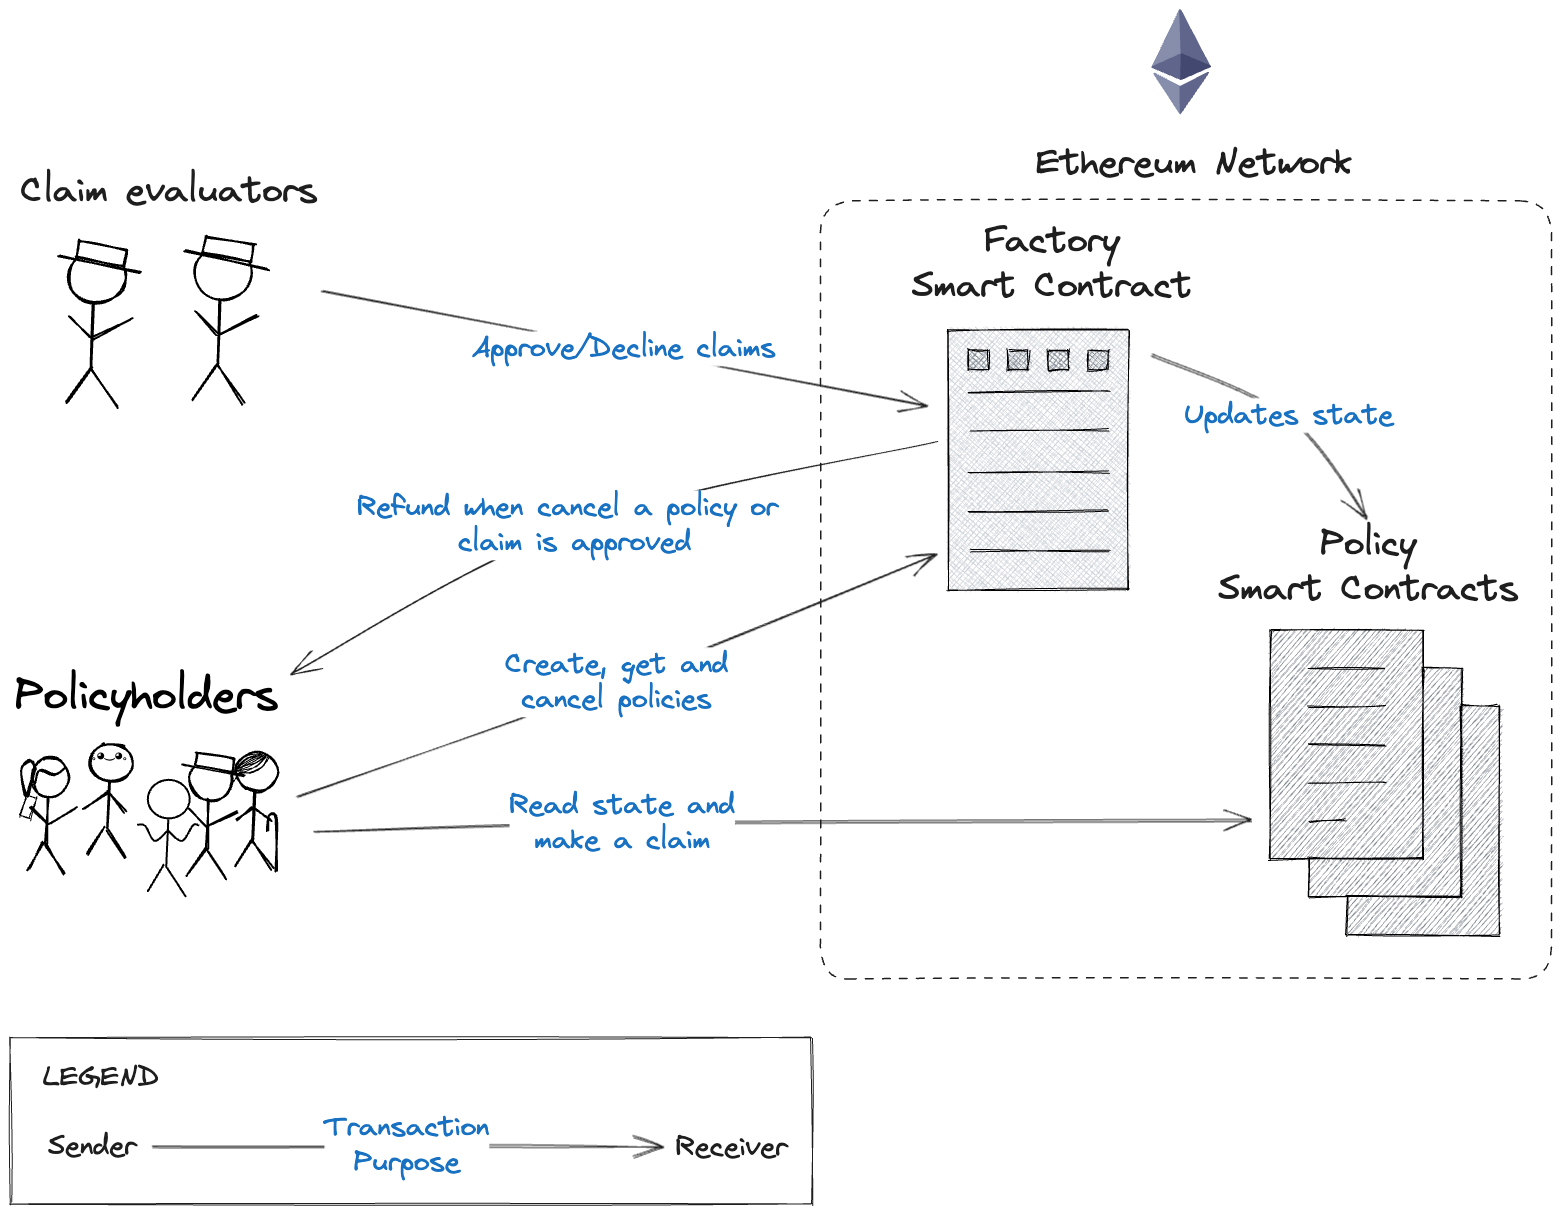
\includegraphics[width=14cm]{img/project-development/factory-policy.png}
\caption[Factory and policy smart contracts transaction flow]{\footnotesize{Factory and policy smart contracts transaction flow}}
\label{fig:smart-contracts-flow}
\end{figure}

The entire code of the Factory smart contract can be found in appendix \ref{appendix:factory-sc}.
}
\subsubsection{Ethereum developer environment}
{
To develop and test smart contracts a developer uses what is well-known as \textbf{testnet}, short for test network. The primary public network is called \textbf{Mainnet} and testing smart contracts here would imply consuming Mainnet \acrshort{eth} on transactions, which requires real money. Therefore, testnets are really useful to test potential smart contracts in a production-like environment before deployment to Mainnet, so it is the analogy to production and staging servers. For the experiment, there were two possibilities:
\begin{itemize}
    \item Use a local testnet, which requires selecting a feature that simulates the Ethereum network locally.
    \item Use a public testnet, which requires asking for testnet \acrshort{eth} to ``faucet entities", which distribute it sometimes free but with daily limitations. 
\end{itemize}

Since the public testnet option requires external dependencies to obtain \acrshort{eth} and the process can be challenging, I decided to use a local testnet through the tool \textbf{Hardhat}.

Hardhat is a tool that lets developers easily deploy contracts, run tests and debut Solidity code without dealing with live environments. Hardhat comes out-of-the-box with \textbf{Hardhat Network}\cite{hardhat_network}. It basically runs a process that implements the \acrshort{evm} and serves JSON-RPC and WebSocket requests. Moreover, it mines a block with each transaction that it receives so this really streamlines the developer experience. On server launch, it provides accounts with the public-private key pairs and a balance of 10.000 Hardhat \acrshort{eth}.

\begin{figure}[H]
\centering
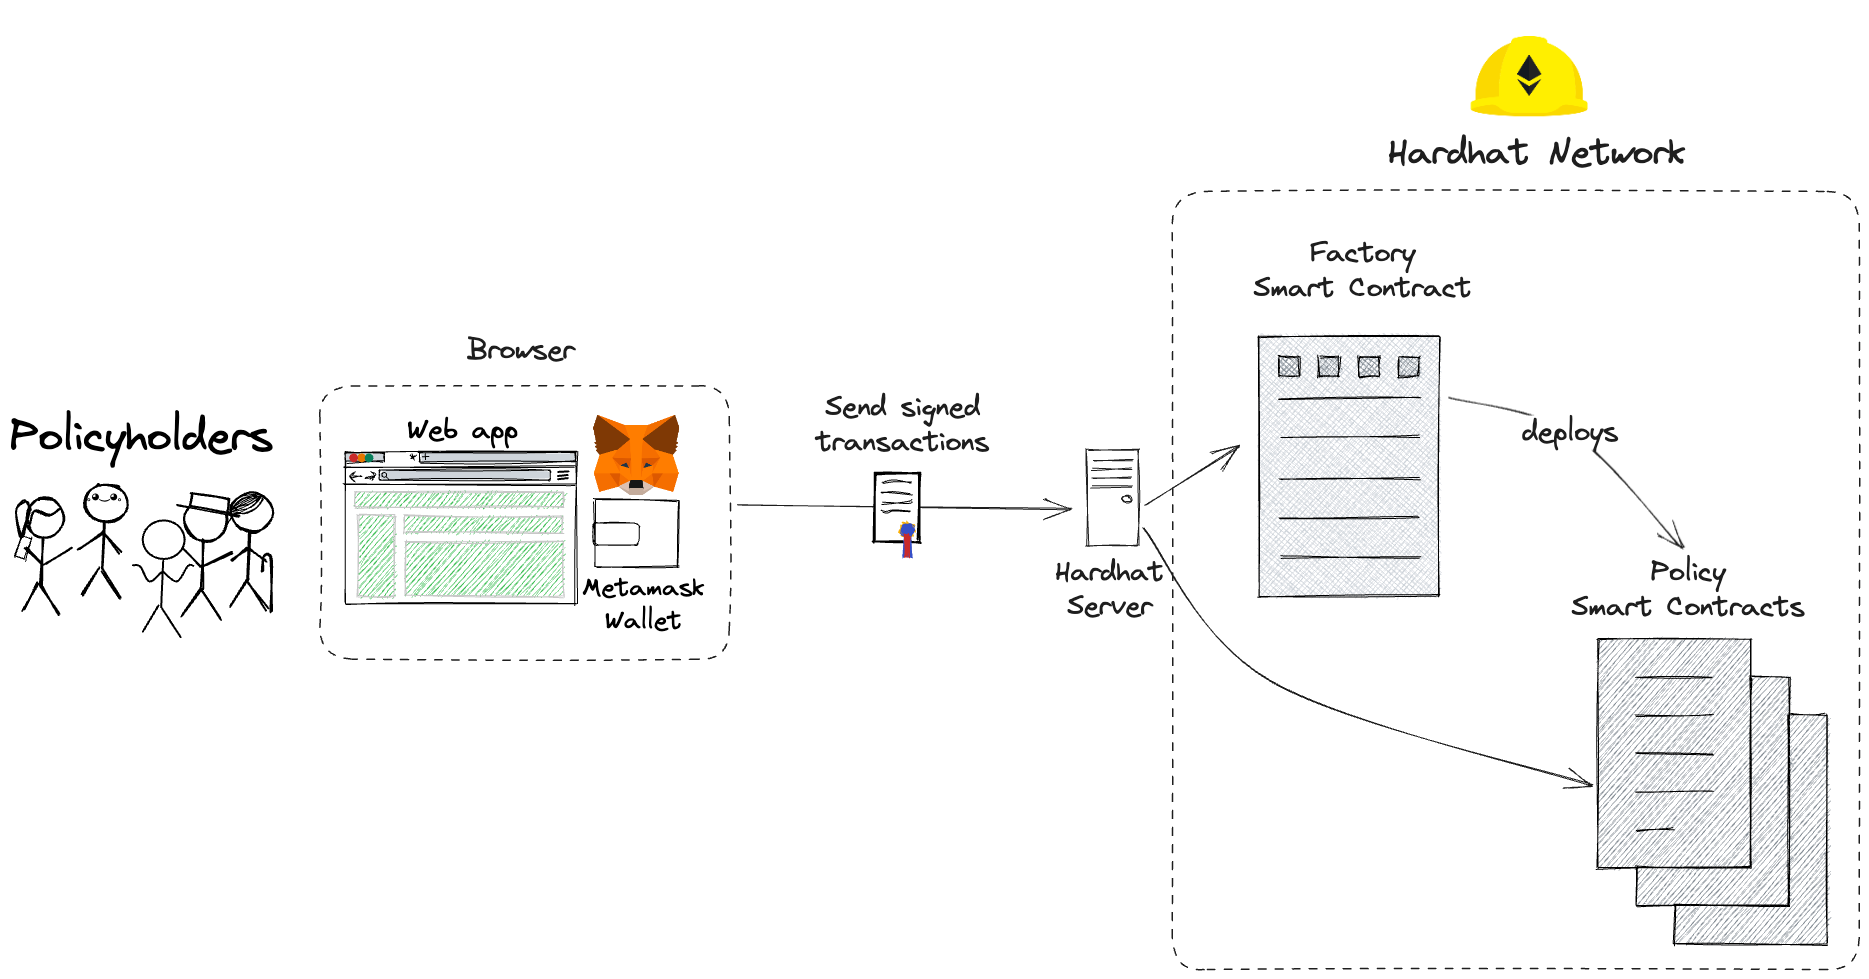
\includegraphics[width=14cm]{img/project-development/hardhat.png}
\caption[Web app consuming Hardhat network]{\footnotesize{Web app consuming Hardhat network}}
\label{fig:hardhat-network}
\end{figure}

In the experiment, the Hardhat network is served at a certain port, where the dapp will deploy the smart contract factory first, and then store the address of such contract into the web app application to make it accessible. As you may observe in figure \ref{fig:hardhat-network}, the web app and the Metamask wallet are configured to reach the factory smart contract and at this point, we are able to request transactions. 

The wallet is in charge of asking for user confirmation on each transaction, so they reach the network signed with the policyholder address. Note that every policy contract deployed through the factory creation process will be in the Hardhat network as well, so they are reachable by the web app too. 

}

\subsubsection{Security consideration}
{
There is an important security issue in this system. The data stored in the smart contracts is public so if it contains sensitive data anyone can see it. We can protect data making private or the getters with modifiers as explained above although, the miners can see all data in the nodes anyway. For our experiment, it does not represent an inconvenience but for a real case this problem could be solved by storing the data encrypted, for example using the public key of the user account to encrypt and the private key to decrypt. This is just a need to protect sensitive data but not necessary for changing the state since function executions can be protected, for instance by the address of the transaction sender.
}


\subsection{Off-blockchain backend}
{
The off-blockchain application consists of a backend app that handles proposal generation by providing pricing and storage of such proposals. There are many possible solutions to implement these requirements but the one selected for me is \textbf{NestJS}\cite{nestjs}.

NestJS is a framework for building efficient, scalable Node.js server-side applications. It is developed with Javascript\cite{javascript} and provides an out-of-the-box application architecture that allows developers to create highly testable, scalable, loosely coupled and easily maintainable applications.

Usually, a backend uses an \textit{\Gls{orm}}, Object-Relational mapping, which provides a way of mapping the data schemas with the backend models and eases the connection and comprehension. For the experiment, I selected \textbf{Prisma}, a new kind of \Gls{orm} which apart from offering really comprehensive documentation and easy implementation with NestJS, recently has grown in popularity because of the way it declares just a data schema as a single source of truth and generates the database and backend types according to this agreement. For the experiment, a \textbf{PostgreSQL}\cite{postgresql} database has been selected, which is a powerful, open-source object-relational database more than enough for storing some proposals.

Thanks to these technologies, I was able to implement the two expected features.

\subsubsection{Proposals module}
{
The goal of the module is to offer insurance coverage and the corresponding price given a specific car and driver data.
In addition, when the user likes the proposal he can save it to purchase it later on. To achieve this the app accepts several requests:
\begin{enumerate}
    \item The first request is through the endpoint \textbf{POST ``/api/proposals/quote"}. The body of this request basically consists of a risk subject and a risk object. The risk subject contains the driver data such as name, document number, and birth date, whilst the risk object collects all detailed specifications about the car. Just a few of this data has been required in favor of the real scenario. Some of these fields are maker and model, plate, fuel type, etc. The response contains the list of coverage services available with their monthly price respectively. 
    \item Once the request wants to be saved, the app offers the endpoint \textbf{POST ``/api/proposals/quote/save"}. The body for this case collects the same attributes as before, risk subject and risk object, but also the coverage configuration the user wants to include on his policy. 
   \item When a user wants to retrieve his saved proposals he can use the endpoint \textbf{GET ``/api/proposals/quote"}. To develop this feature the authentication module has to be implemented, which is explained in the section \ref{section:authentication-module}.
\end{enumerate}

With the previous endpoints, we enable the web app to ask for the data from the user and request the backend for a quote pricing. Once the backend responds, the coverage possibilities may be displayed to the user who then selects the coverage services that he would like to include. Eventually, if the proposal sounds good to him, he could save the proposal. The following step was to implement the authentication module to bind the proposals to the clients.
}

\subsubsection{Authentication module}
\label{section:authentication-module}
{
The authentication flow proposed for the dapp is a little bit different from the standard models since it uses the client wallets instead of a social media login or the usual email/password combination to identify a user.

Since we are using blockchain and we can assume each of our clients has an address, we can leverage these authentication credentials to identify them in our backend. The concept is called \textbf{nonce-based authentication} and is quite simple:
\begin{enumerate}
    \item A user wants to be authenticated so he asks the backend to generate a \gls{nonce}. The backend app generates the nonce and stores it for some time. Theoretically, this nonce cannot be generated again so each time is requested the app generates a different one. To generate this nonce it was used the library \textit{Siwe, Sign in with Ethereum}\cite{how-siwe}.
    \item Then, the user receives the nonce and signs it using his private key. Once signed he sends to backend the signed message along with the public key.
    \item Backend verifies that the message has been signed with the public key received and it contains the nonce provided previously, so it guarantees that the sender is the owner of the private key, the unique capable of signing the message, hence it is authenticated. The nonce gets removed from the backend storage and a token for authenticating the account is returned to the user in order to attach it to the headers and access protected endpoints.
\end{enumerate}
This behavior is achieved with two endpoints: \textbf{GET ``/api/auth/generate-nonce"} and \textbf{POST ``/api/auth/authenticate"} as you may observe in figure \ref{fig:auth-flow}. At this point, the backend app can protect the endpoint for saving proposals, so the proposals will be always sent with an authentication header including the token that identifies the user and we can bind the proposal to him.

\begin{figure}[H]
\centering
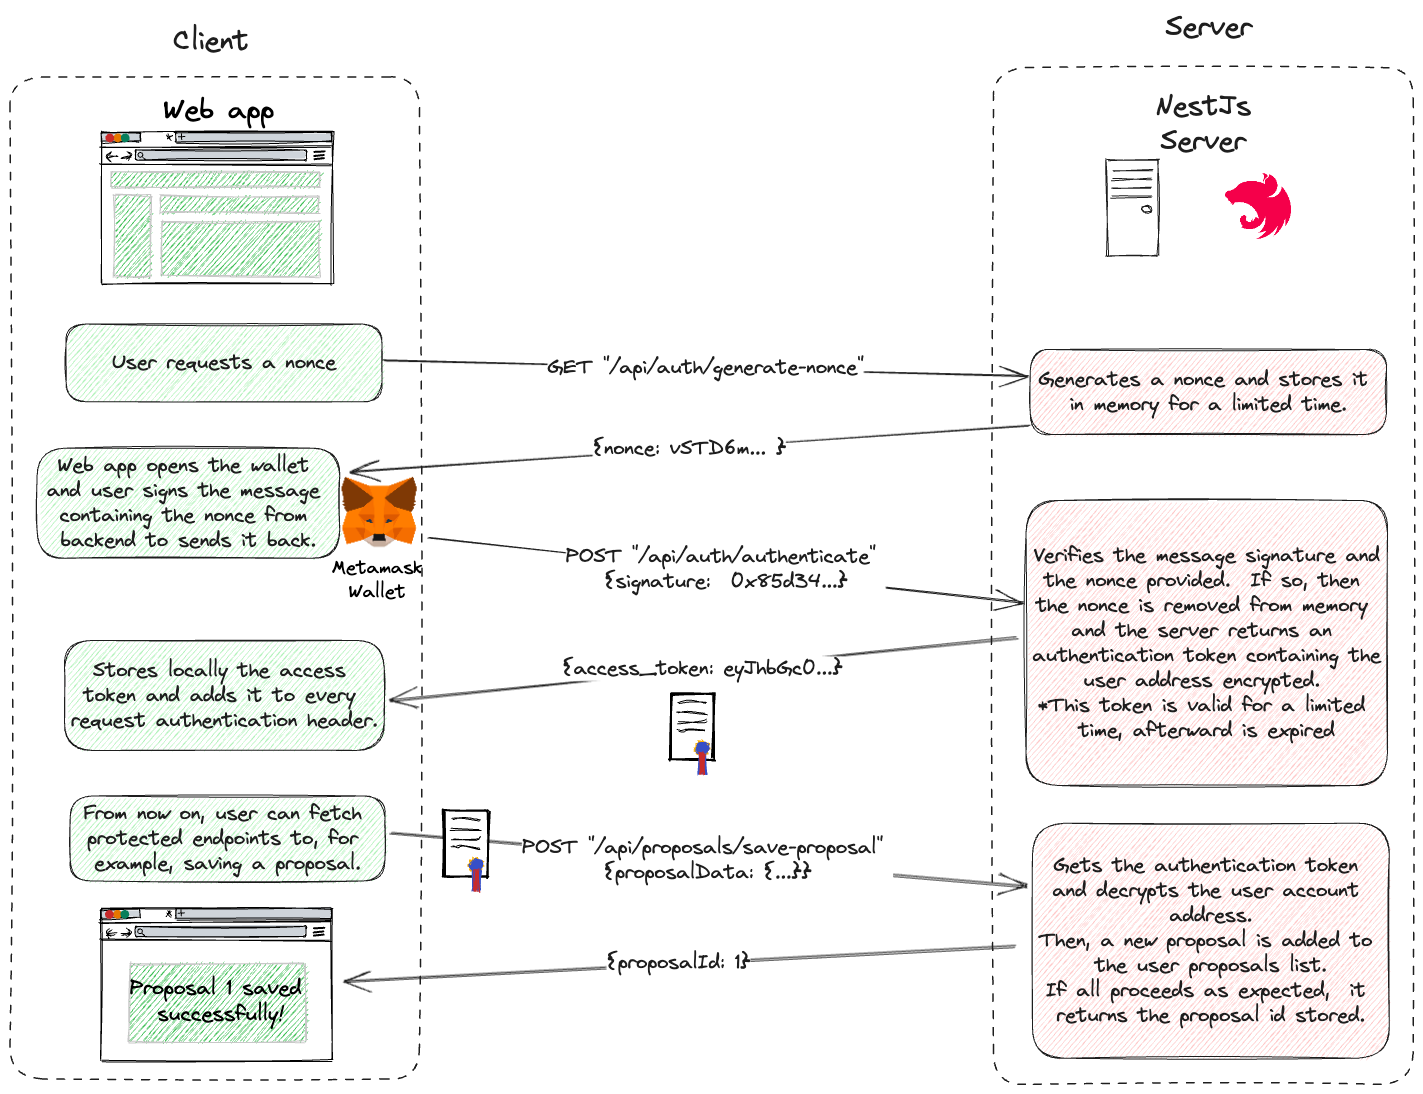
\includegraphics[width=14cm]{img/project-development/nonce.png}
\caption[Authentication flow]{\footnotesize{Authentication flow}}
\label{fig:auth-flow}
\end{figure}

In addition, the endpoint to get user proposals must be protected as well so it requires the authentication token. Therefore, when the backend app receives a request, it checks the token, gets the account and retrieves the list of proposals for that user. This idea of authenticating through the Ethereum account is based on the articles \cite{how-siwe} and \cite{why-siwe}.

}
}

\subsection{Frontend}
{
The frontend app is the last piece to complete the system. It aims to provide a platform for the users that want to interact with the dapp. Moreover, it will be the unique software to interact with both, off-blockhain and on-blockchain backends.

There are many technologies to develop a frontend web application. For the experiment, I selected \textbf{Next.js}. Next.js is a \textbf{React}\cite{reactjs} framework to create full-stack web applications that include out-of-the-box features to compile, bundle and build the application which reduces widely the time spent in configuration. This is one of the most common solutions adopted by the frontend community.

React, like most of the libraries to develop web applications, is based on the idea of building User Interface (UI) components and composing them like a tree with nodes in the DOM in order to eventually create interactive pages as is represented in the figure \ref{fig:react-dom}. Such components can be compared to math functions, which receive input data and return visual elements that are displayed in the browser. 

In addition, components can pass data to other components and react to user interactions such as clicking a button or filling out a form. Every event or change triggers a render which means the component is computed again to display the change in the layout and it propogates the change to the child components. React counts on a really efficient algorithm called ``\textit{Virtual DOM}" to compute the changes between two renders and display the new UI immediately in the browser \Gls{dom}. 

\begin{figure}[H]
\centering
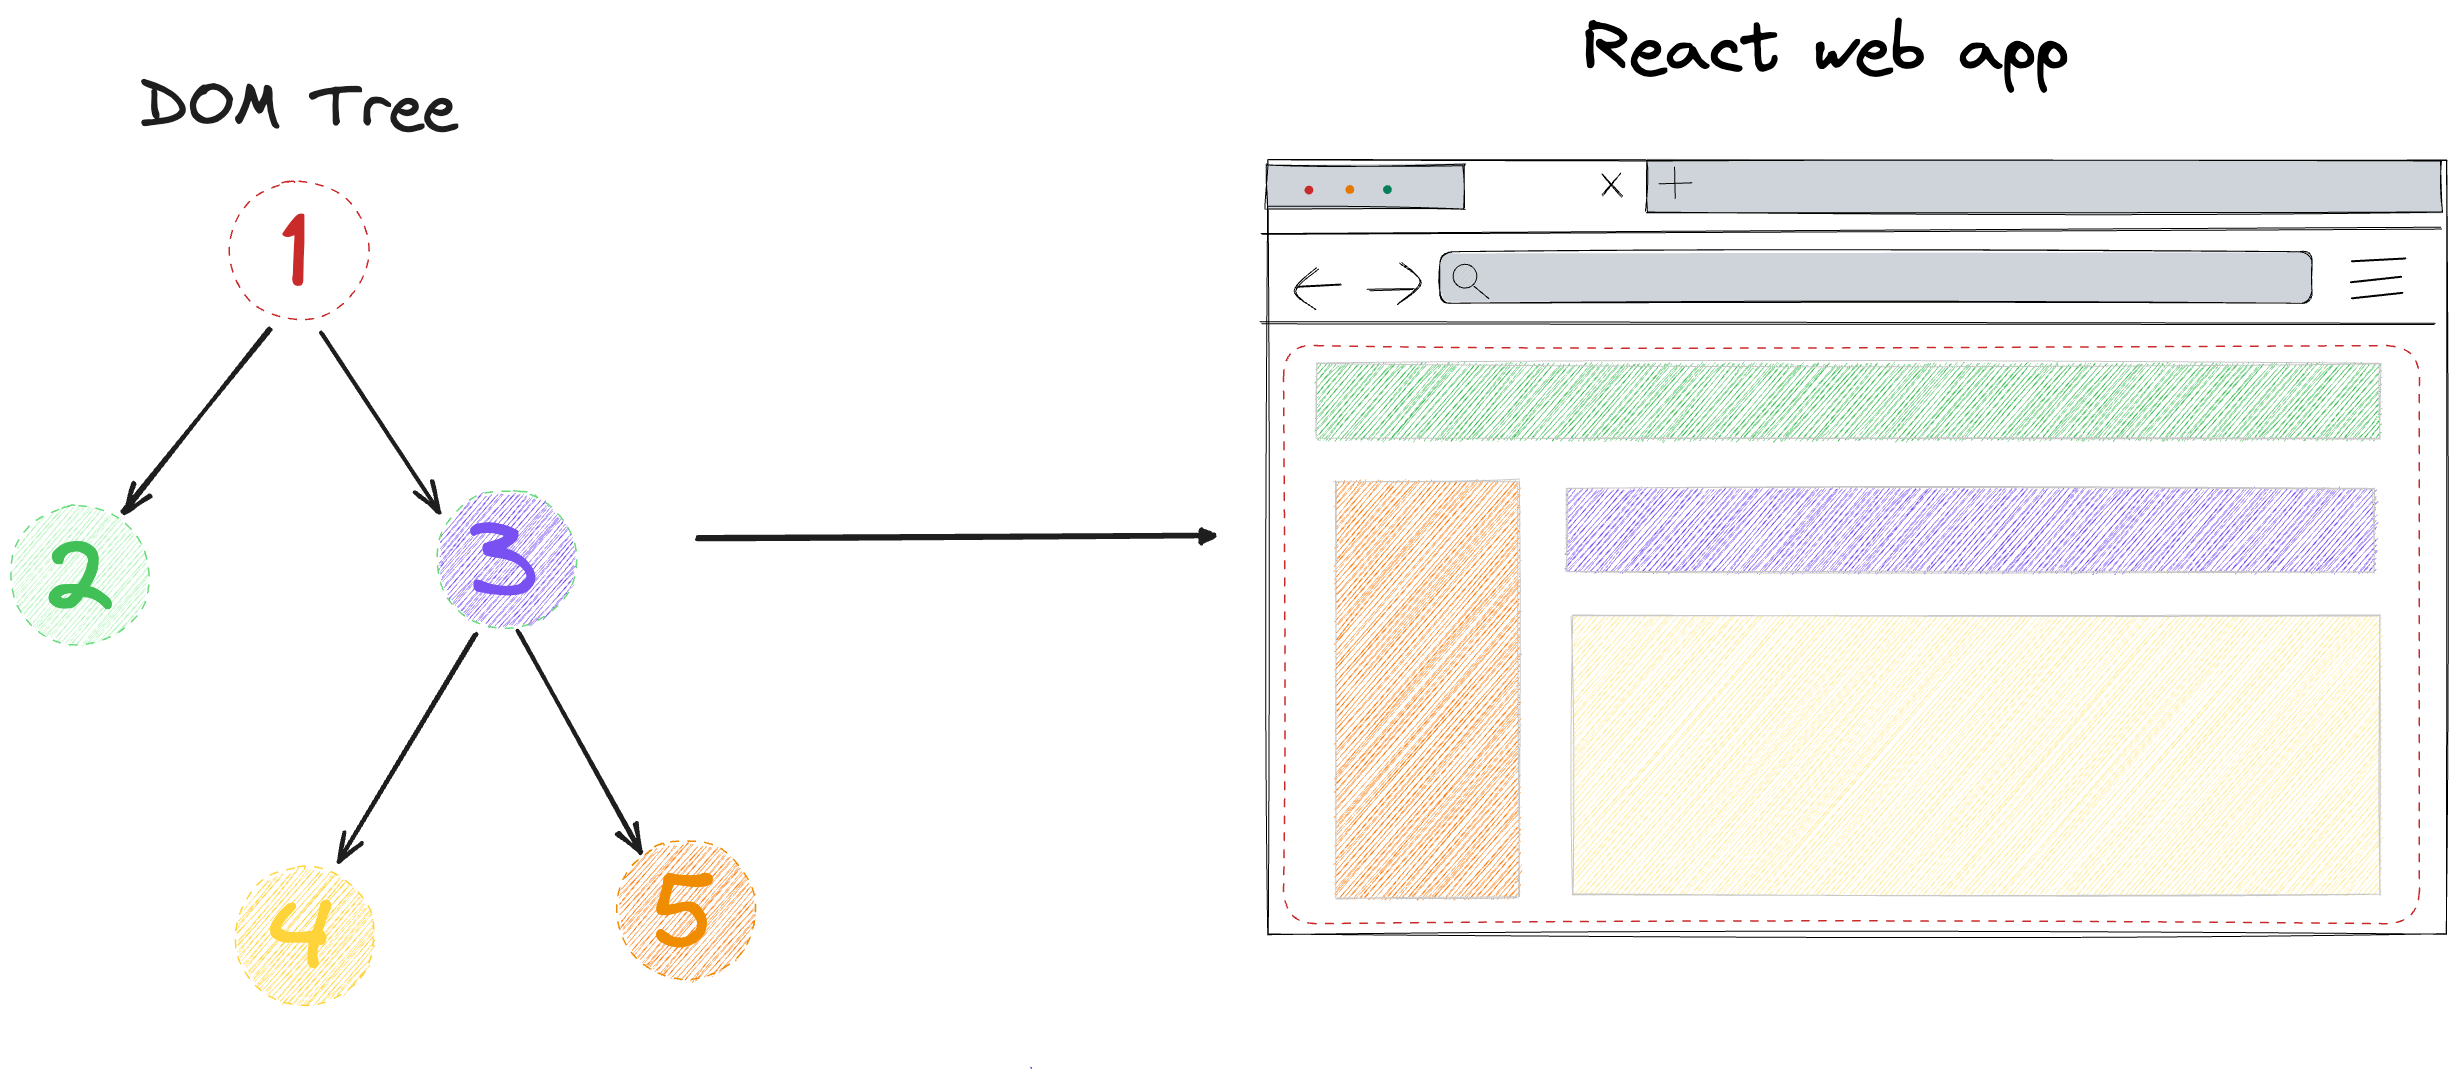
\includegraphics[width=14cm]{img/project-development/react-dom.png}
\caption[React tree to browser DOM]{\footnotesize{React tree to browser DOM.}}
\label{fig:react-dom}
\end{figure}

Next.js provides a powerful layer which is known as \textbf{Server side rendering (SSR)}. As you may see in figure \ref{fig:ssr}, when the user requests a web page SSR server pre-renders the content in the server and responds with the first version rendered to the client. This significantly enhances the user first-load experience and page indexation in browser engines. Once the app is displayed on the client, the next renders happen on the client side. 

\begin{figure}[H]
\centering
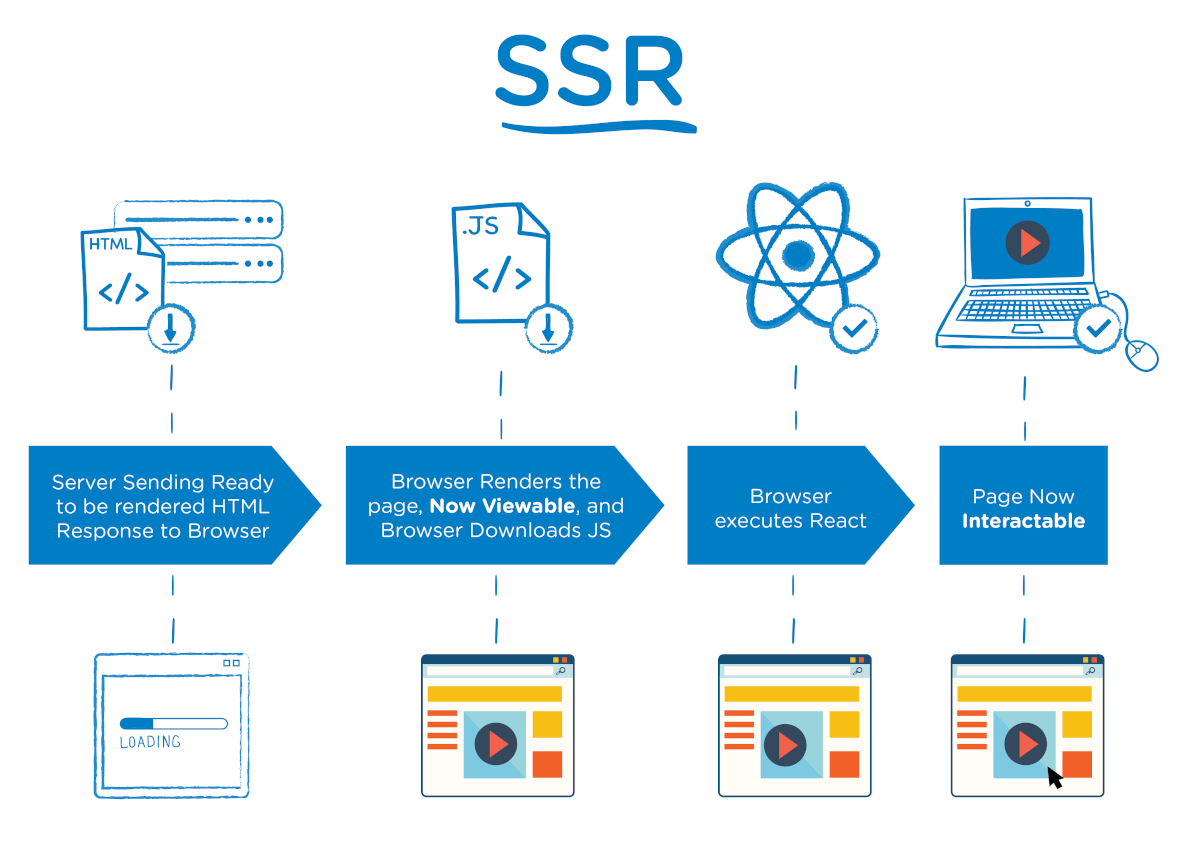
\includegraphics[width=14cm]{img/project-development/ssr.png}
\caption[Server side rendering of web applications]{\footnotesize{Server side rendering of web applications.}}
\label{fig:ssr}
\end{figure}

The project has used libraries like \textit{Material UI}\cite{mui}, which provide a huge amount of stylish and pretty components that can be used to ease the design and development process resulting in a more fancy layout. About the blockchain part, it consumes the ABI's generated by the contracts compilation and along with the Javascript libraries \textit{wagmi.sh} and \textit{ethers.js}\cite{ethers}, the communication with the smart contracts and the wallet becomes pretty straightforward.
}


\subsection{Version control}
{
All the code of the project has been stored in \textbf{Github}\cite{github}, a cloud version control storage that allows us to host our \textbf{Git} repository. Git\cite{git} is an open-source version control system worldwide used by developers to work with code in a traceable, organized, and clean way. It lets the developers access all the codebase history, creating incremental versions and forking to try different ideas but also merge when necessary.

Having all the code centralized in a single source of truth, which let me create different versions or approaches of the experiment was fundamental to not blocking the progress of the project and working on several features without breaking a stable incremental version.
}

%%% RESULTS %%%
\clearpage\section{Results}
{
Eventually, the dapp took shape thanks to the combination of the technology explained in the previous section. By using the backend on-blockchain, the backend off-blockchain, and the frontend web application, I have built an accessible web app that lets standard users the possibility to contract a car insurance policy with blockchain empowered capabilities, such as ownership and censorship-resistance. The clients can read the policy contract before confirming the purchase and make it clear what the company can and cannot do. All the operations are transparent and there is even a trace of all computations carried out so the blockchain model enhances the situation of the traditional model. The dapp project has been called \textbf{Insurechain}, mixing the words ``blockchain" and ``insurance".


}
\subsection{Dapp software overview}
{
The resulting software stack of the dapp may be cumbersome. It relies on every piece in charge of some specific tasks that combined with the other pieces deliver a comprehensive and valuable product. To have a clear idea of the elements involved we can take a look at the figure \ref{fig:dapp-overview}.

\begin{figure}[H]
\centering
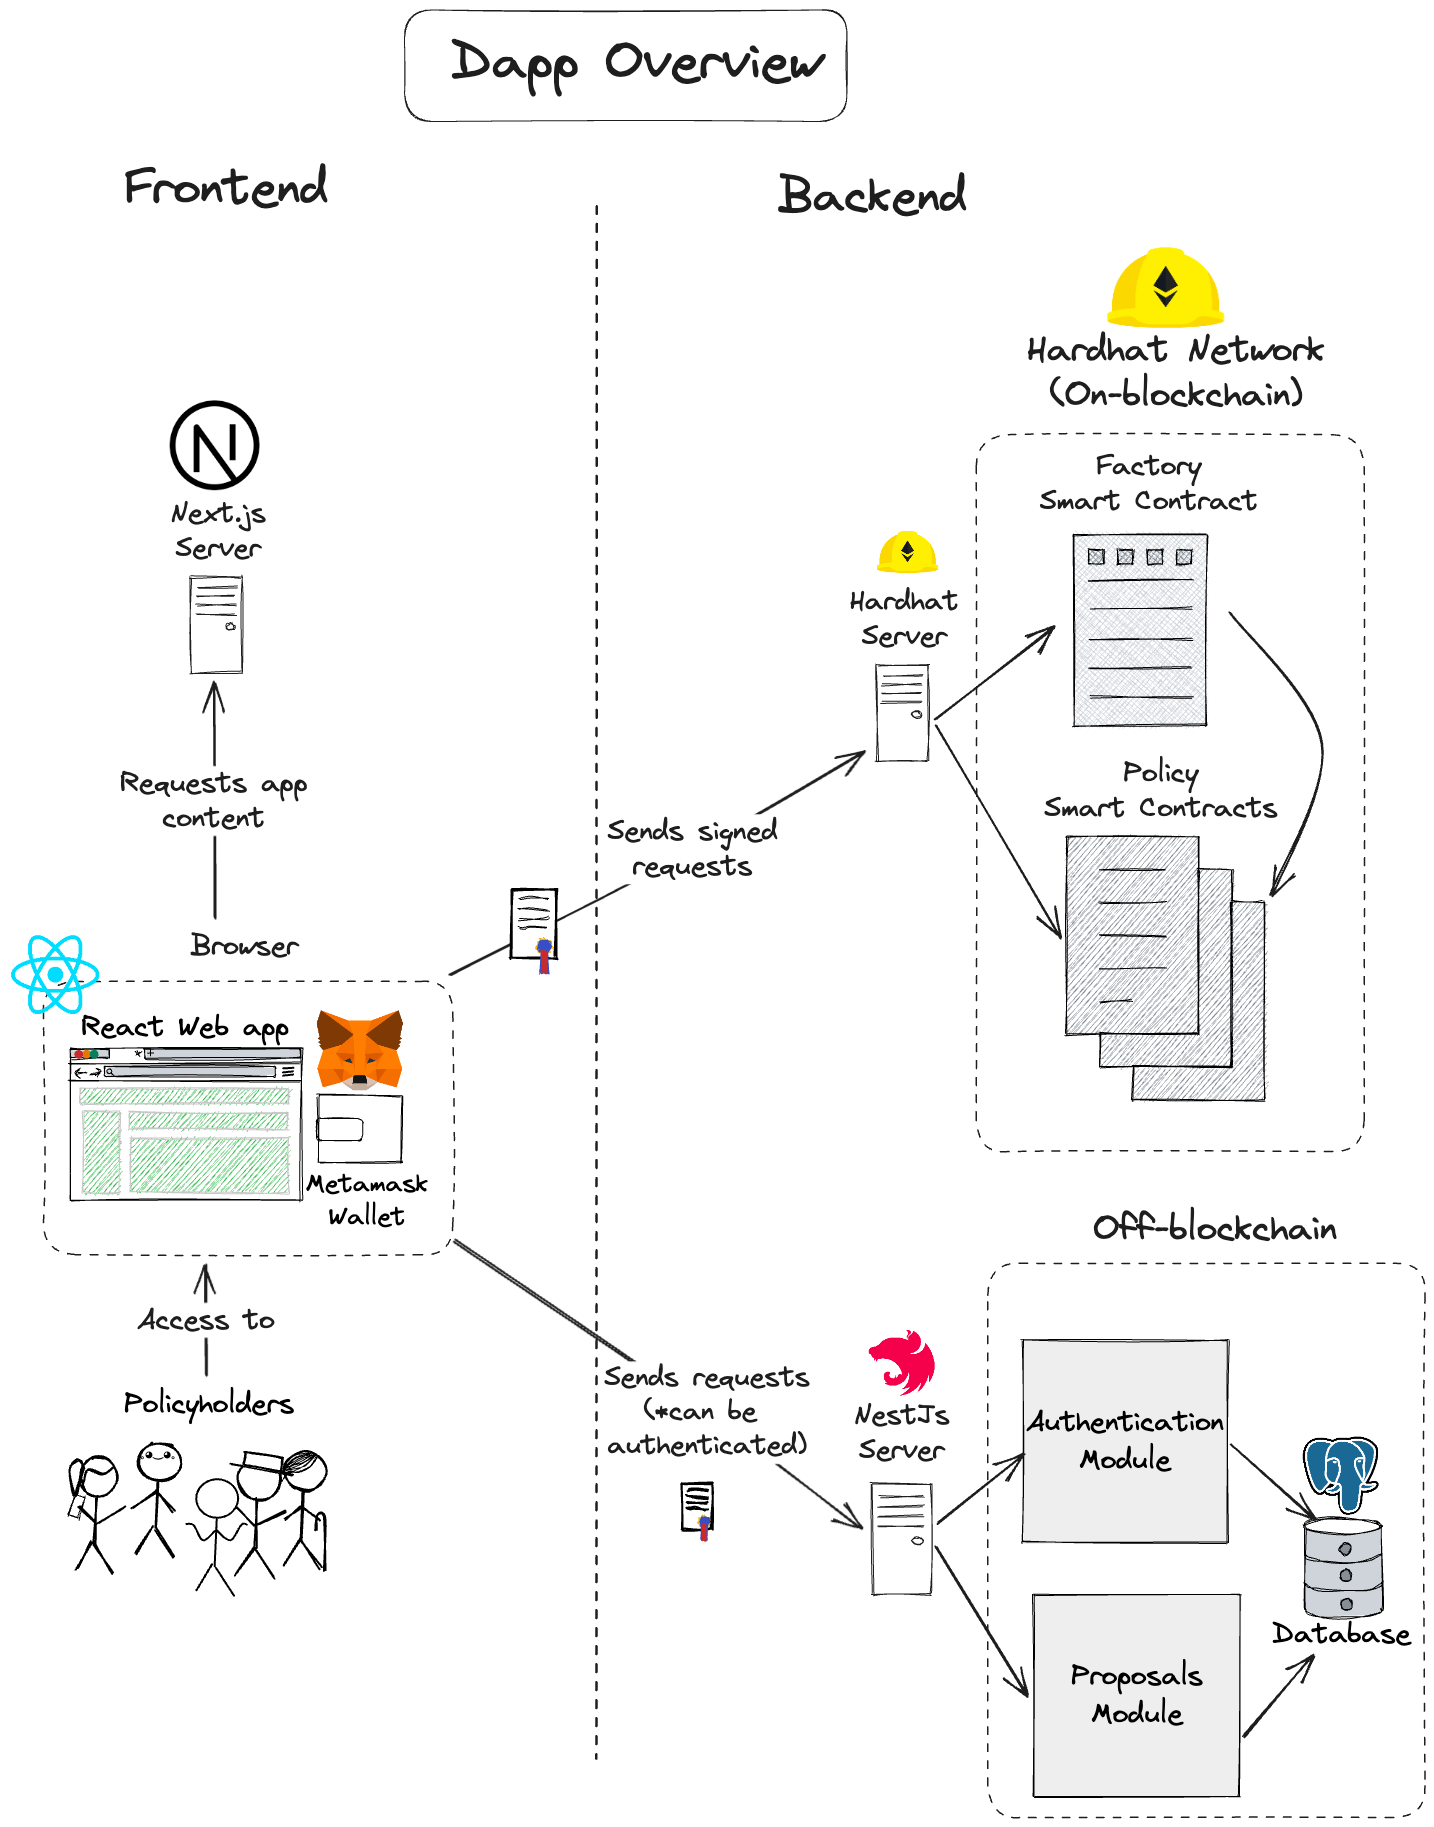
\includegraphics[width=14cm]{img/results/dapp-overview.png}
\caption[Dapp software overview]{\footnotesize{Dapp software overview.}}
\label{fig:dapp-overview}
\end{figure}

There are some insights to highlight in this breakdown:
\begin{itemize}
    \item The policyholders can easily access the dapp through the web app technology and a wallet such as Metamask. The Next.js server is responsible for delivering the UI that the web app demands to display the data properly.
    \item The communication with the backend can be authenticated or not depending on the moment the user signs in using the wallet. This way, the identification of a user is the same for both backend pieces: the user address. Although the Ethereum transactions get signed by protocol automatically, the NestJs server verifies as well the user by the authentication flow based on ``Siwe".
    \item The Nestjs server protects some endpoints according to the need to create data bound to a specific user address. 
    \item The Nestjs modules rely on the relational database to store all the proposals list of the users, where the primary key is their account address. In this manner, we prevent the user from consuming gas, i.e. spending money, just to create a proposal, which from the product point of view does not make any sense. Hence, creating proposals does not have any blockchain effect.
    \item The web application can display all proposals of a user. If a user wants to purchase one, this transaction is emitted to the Hardhat network when the Factory smart contract is deployed. There, it creates and deploys a Policy smart contract and returns the deployment address. Metamask helps the user by displaying the transaction details and prompting them to confirm the execution.
    \item Since the Factory smart contract stores data from all the policies created for each user, every user can get their policy details on the web application. 
    \item The policyholders can perform actions on the policy smart contract. The web app application has implemented the cancel method which requires the minimum computational gas to confirm the transaction.
\end{itemize}

I would like to emphasize that the backend parts do not communicate between them intentionally. Each part is in charge of storing a certain part of the business logic that has been thought for. It is beyond the scope of this experiment to make an interface for the company and evaluators, because it is a matter of fact that converting the policyholder flow proves that the conversion to the blockchain model is feasible from the other parts too since it is streamlining the communication for all parts concerned. Furthermore, from the point of view of the company, it also offers a lot of value since users have to pay to operate over the policy which represents a first barrier for reducing fraud but also there are incredible possibilities to rely on the blockchain such as trust the risk computation to the network so the policyholders cover themselves, therefore the proposal quote price and renewals regulates automatically depending on historical accident rate.
}

\subsection{User experience flows}
{
In this section, we can find the resulting user experience flows of what a policyholder is facing when he opens the Insurechain web application to obtain a car policy. To make explanations more clear and accurate, during this whole section the on-blockchain part is referred to as smart contracts, the off-blockchain part as the backend, and the frontend part as the web app.
}

\subsubsection{Landing page}
{
Every web application has a landing page. This page is where a new user usually "lands". There, he may find all the information about what the product does and which are its benefits. Moreover, the company is introduced to the client. In so doing, the user can make a quick idea about what the company offers to him. For Insurechain, I simulated what could be a landing page, as you may see in figures \ref{fig:landing-1}, \ref{fig:landing-2}, \ref{fig:landing-3} and \ref{fig:landing-4}.
\begin{figure}[H]
\centering

\includegraphics[width=14cm]{img/results/landing-1.png}
\caption[Landing page - part 1]{\footnotesize{Landing page - part 1.}}
\label{fig:landing-1}
\end{figure}

\begin{figure}[H]
\centering
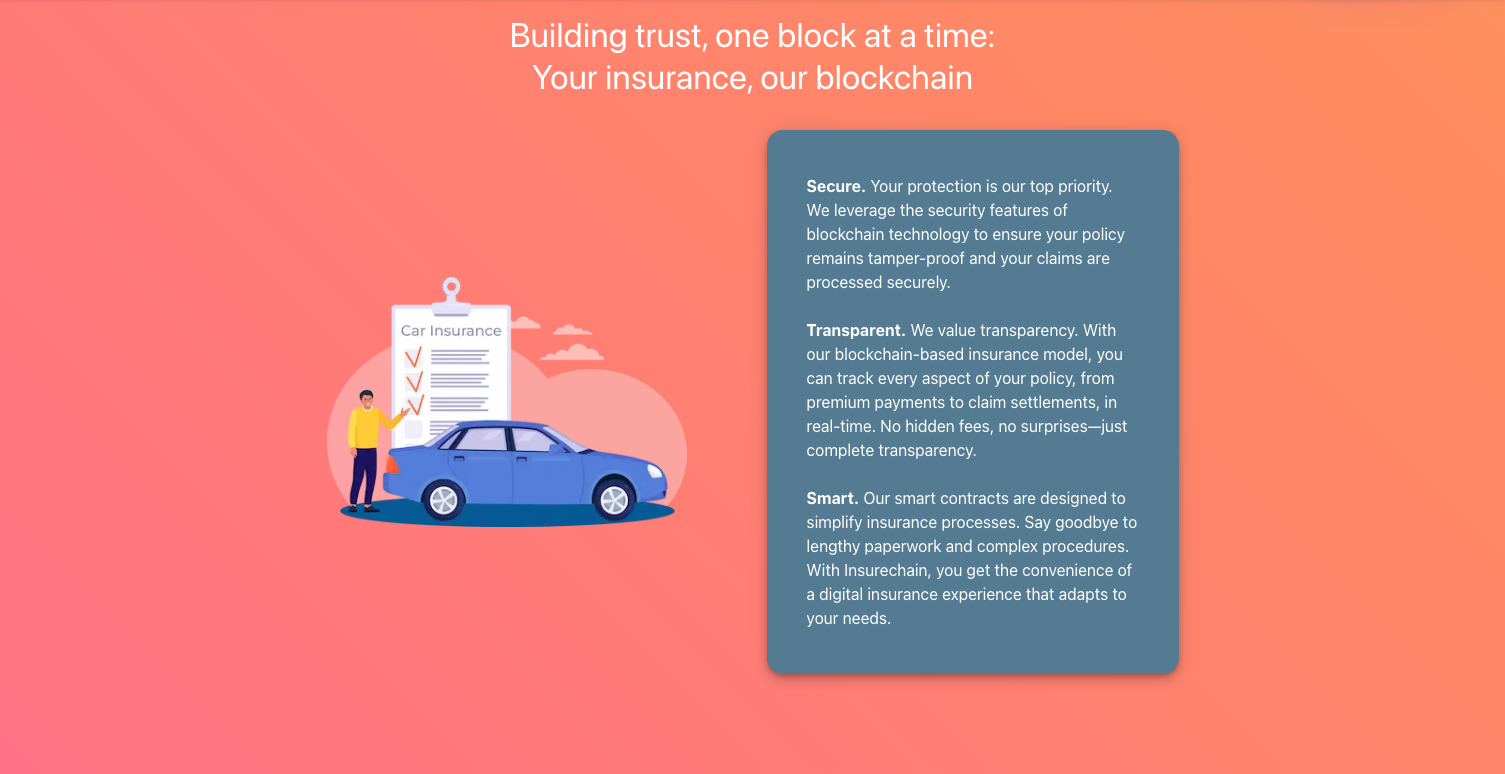
\includegraphics[width=14cm]{img/results/landing-2.png}
\caption[Landing page - part 2]{\footnotesize{Landing page - part 2.}}
\label{fig:landing-2}
\end{figure}

\begin{figure}[H]
\centering
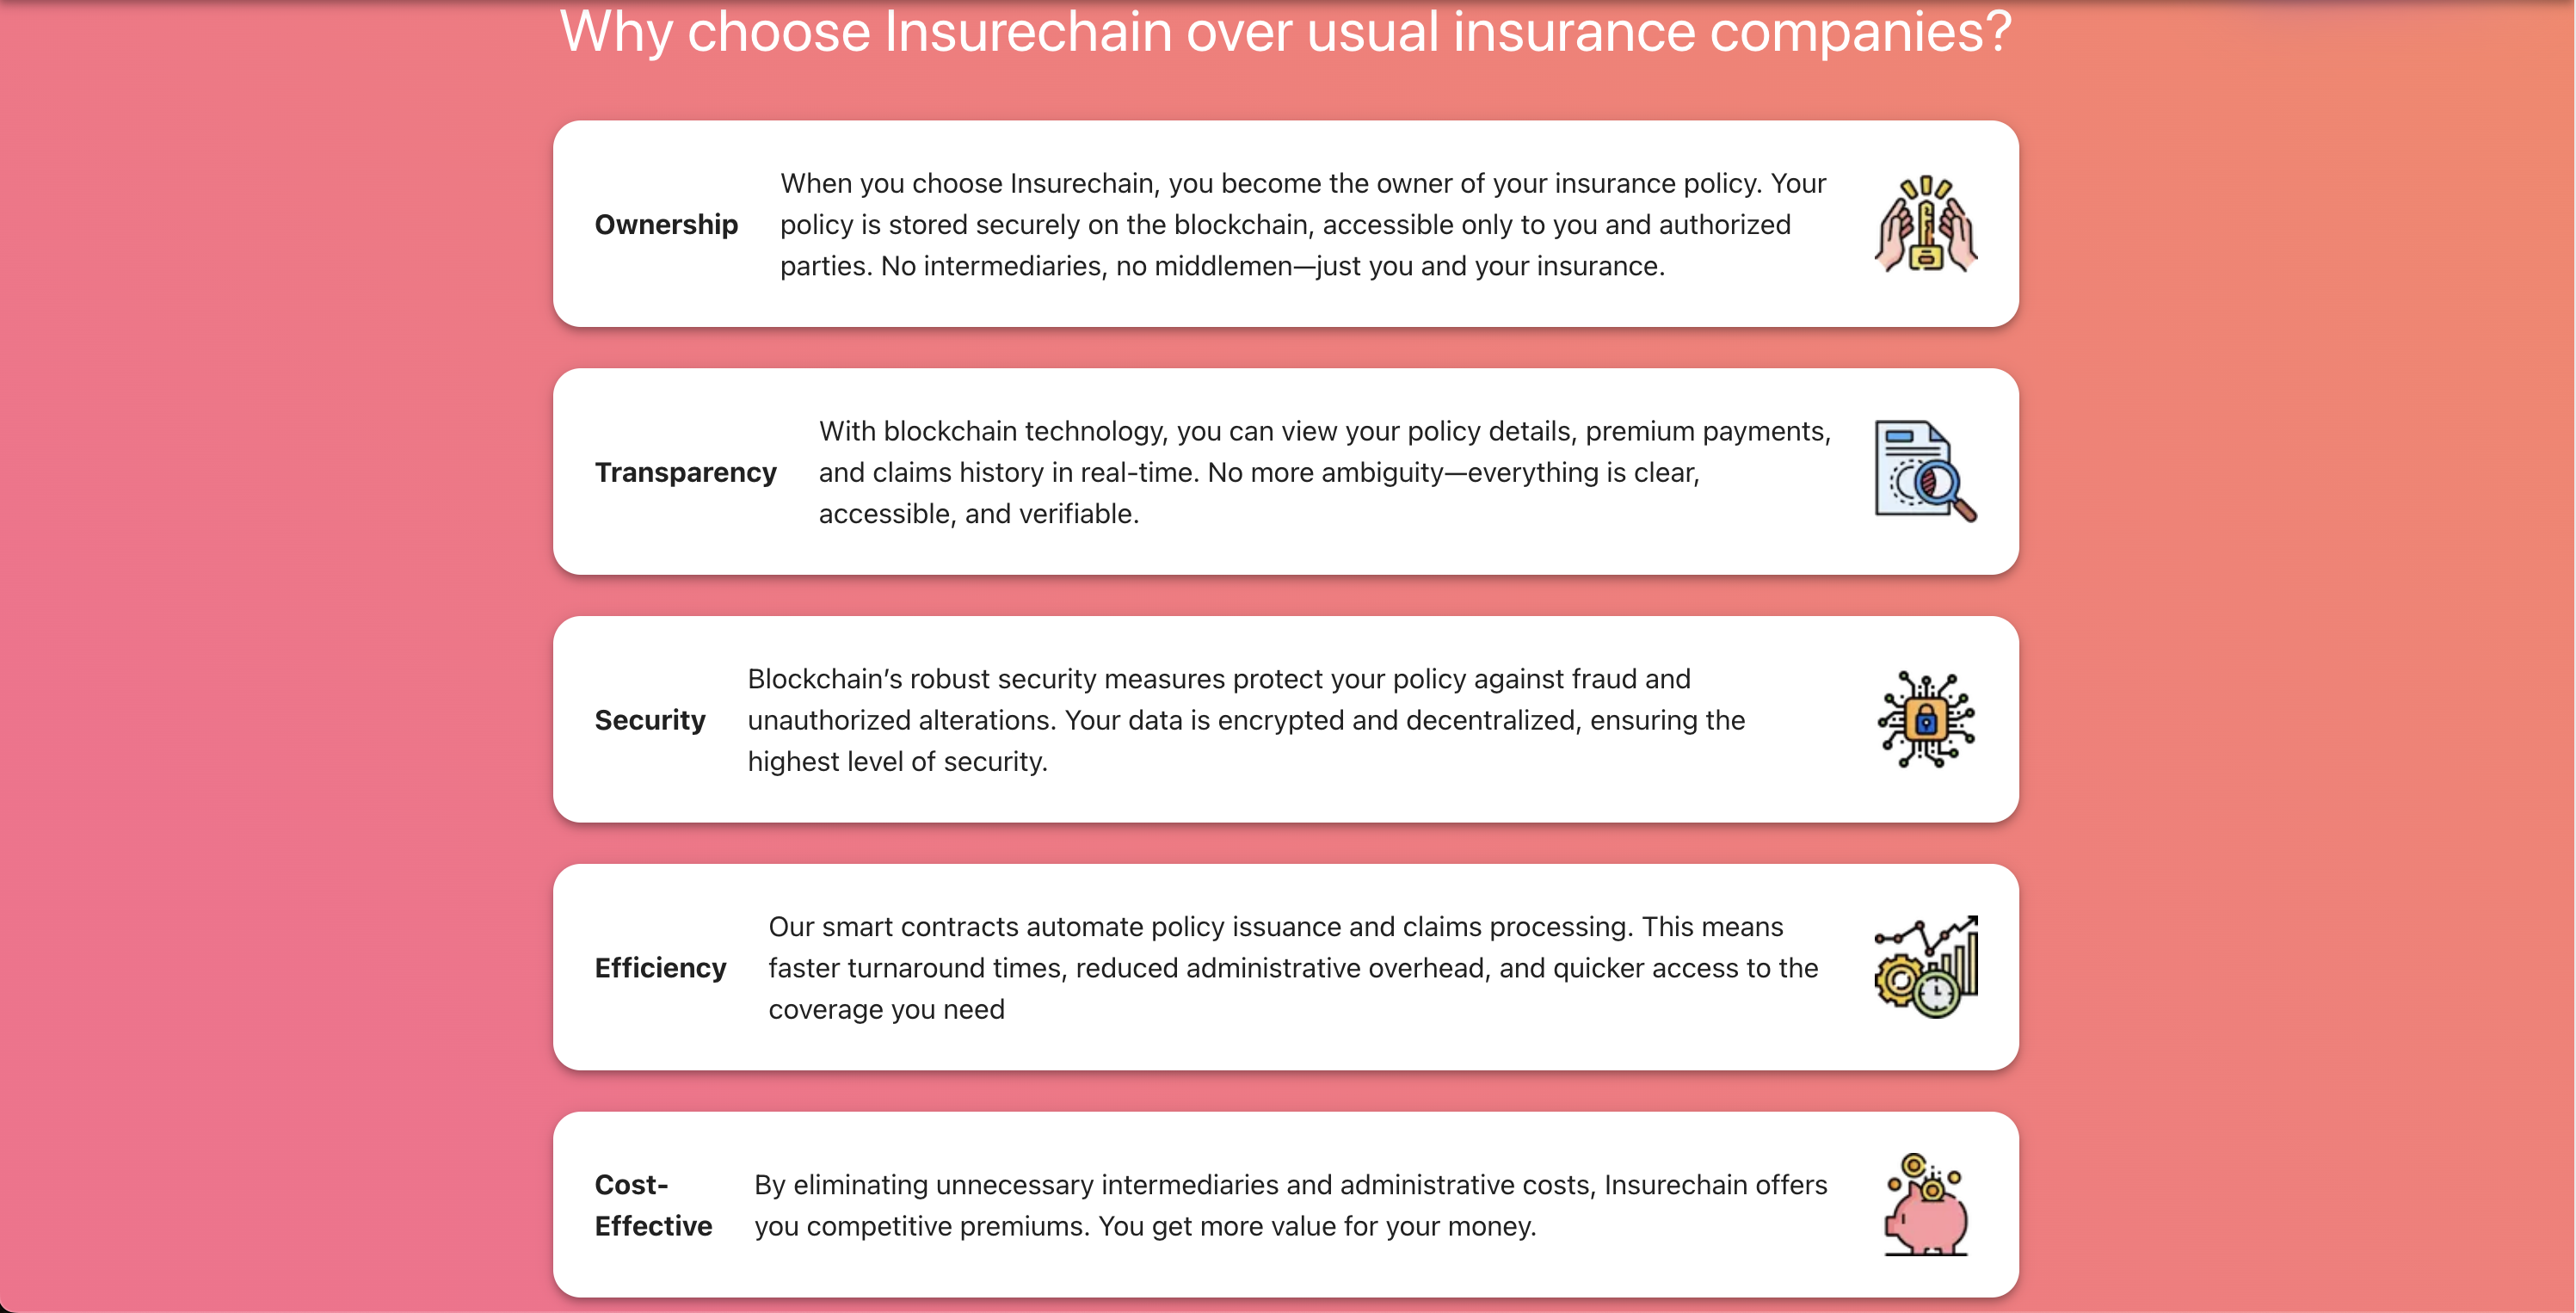
\includegraphics[width=14cm]{img/results/landing-3.png}
\caption[Landing page - part 3]{\footnotesize{Landing page - part 3.}}
\label{fig:landing-3}
\end{figure}

\begin{figure}[H]
\centering
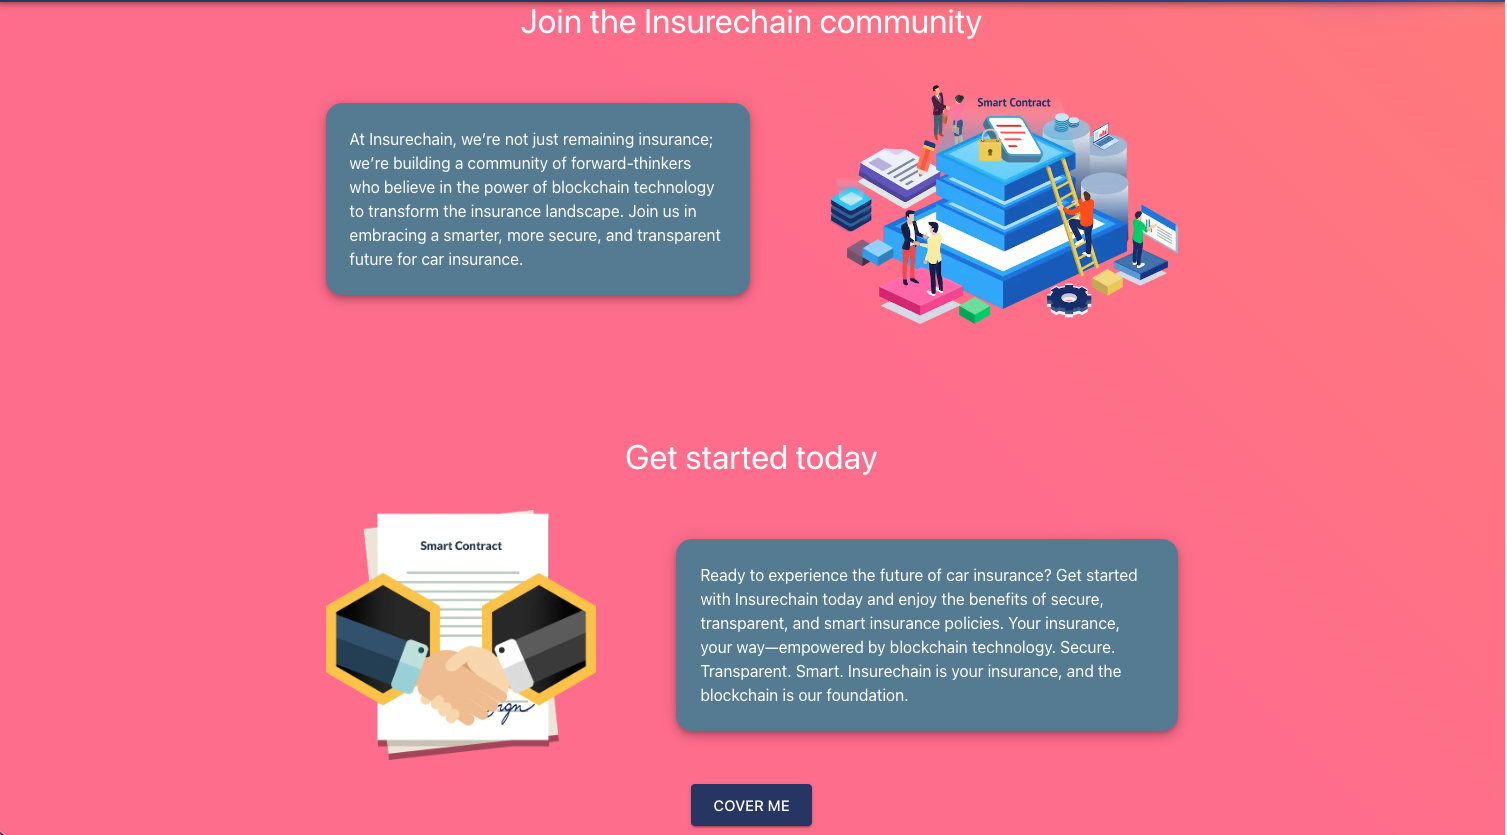
\includegraphics[width=14cm]{img/results/landing-4.png}
\caption[Landing page - part 4]{\footnotesize{Landing page - part 4.}}
\label{fig:landing-4}
\end{figure}

As you may see, there is a basic but comprehensive explanation of what the product achieves and the advantages for the user. Finally, the user can find a ``Call to action" button to begin the process of creating a proposal.
}

\subsubsection{Login}
{
In the header, which is the fixed toolbar located at the top of the page that you can see in figure \ref{fig:header-toolbar}, we may find the Insurechain logo, a link "Car Insurance" which navigates to the Car insurance proposal enrollment. In addition, on the right side, we may find a button that says "Connect Wallet".
\begin{figure}[H]
\centering

\includegraphics[width=14cm]{img/results/header.png}
\caption[Insurechain: Header toolbar]{\footnotesize{Header toolbar.}}

\label{fig:header-toolbar}
\end{figure}

Clicking on the "Connect to wallet" displays the available wallets installed in your browser. Each client is supposed to choose one. In the experiment, we have used Metamask as you may see in figure \ref{fig:wallet-list}. 

\begin{figure}[H]
\centering
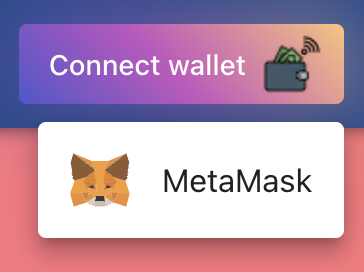
\includegraphics[width=5cm]{img/results/auth-wallet-list.png}
\caption[Insurechain: Available wallets]{\footnotesize{Available wallets.}}
\label{fig:wallet-list}
\end{figure}

When selecting Metamask, a new pop-up will raise to provide permissions to the web app for accessing the wallet data as shown in figure \ref{fig:grant-permission-to-wallet}.

\begin{figure}[H]
\centering
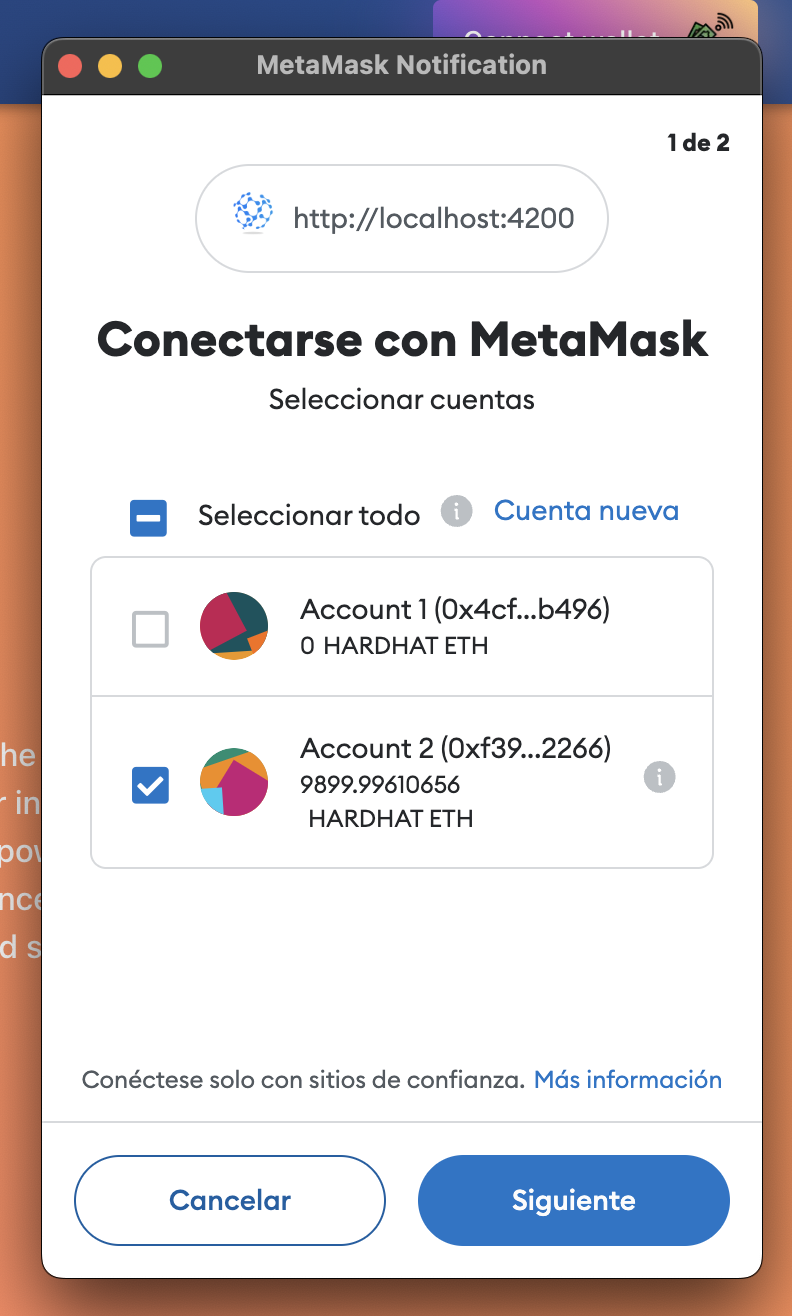
\includegraphics[width=6cm]{img/results/auth-metamask-connect.png}
\caption[Insurechain: Metamask granting access to selected accounts ]{\footnotesize{Metamask granting access to selected accounts}}
\label{fig:grant-permission-to-wallet}
\end{figure}

Once the user has granted the permissions to the app to consume the wallet account data, the frontend immediately requests a nonce to the backend and displays a modal where the user is asked to confirm the signing message as you can see in figure \ref{fig:metamask-sign-in}.

\begin{figure}[H]
\centering
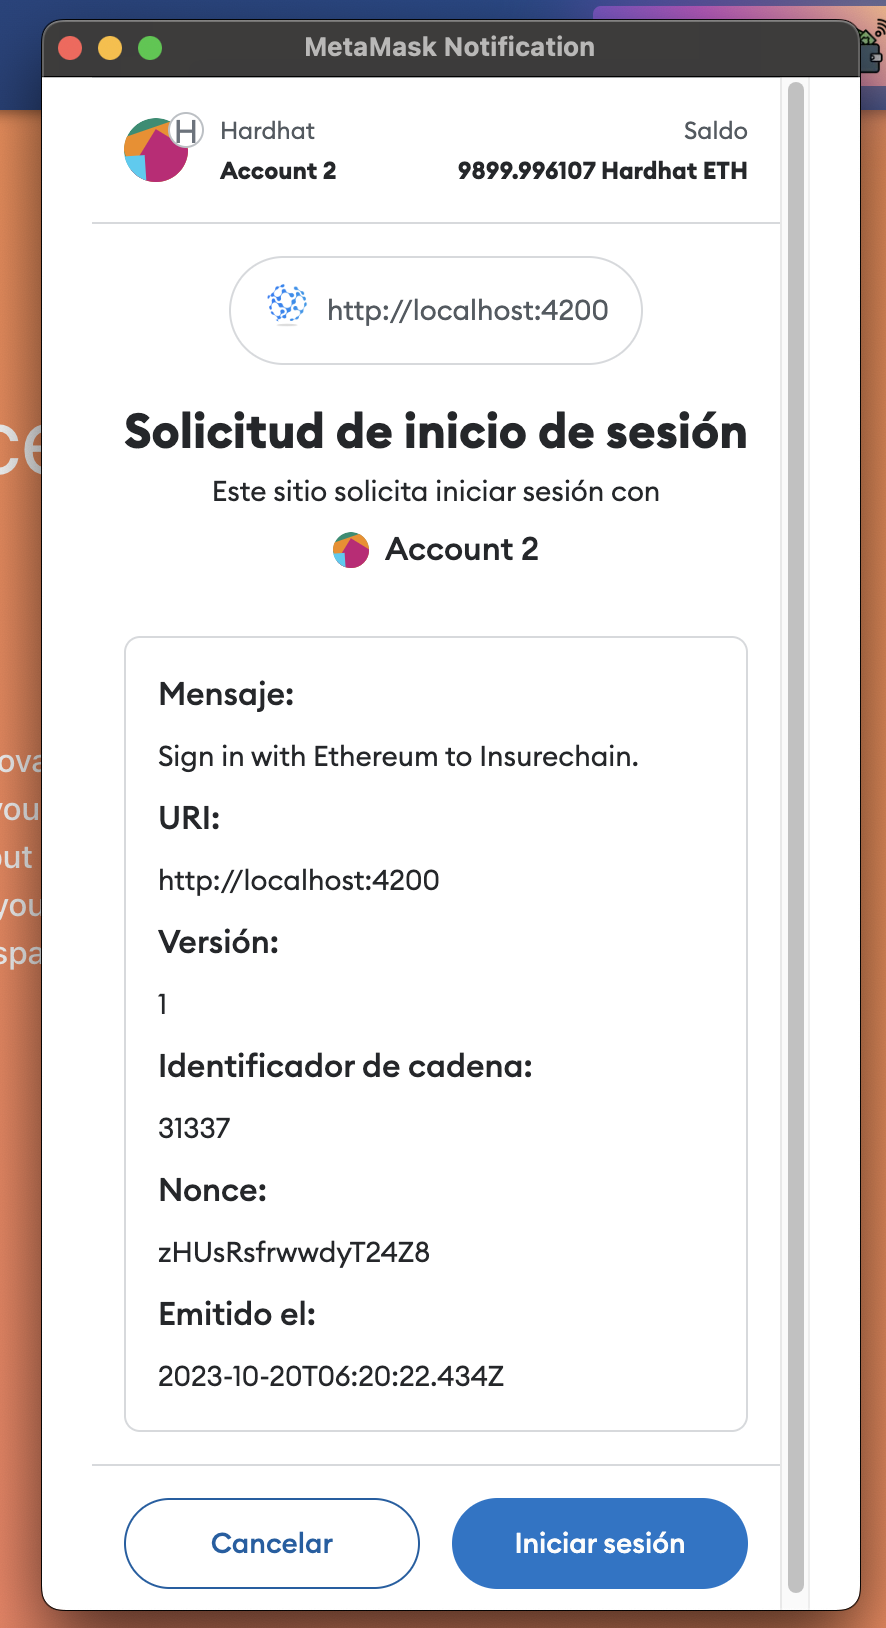
\includegraphics[width=6cm]{img/results/auth-sign-in.png}
\caption[Insurechain: Metamask prompting to sign the sign-in message ]{\footnotesize{Metamask prompting to sign the sign-in message.}}
\label{fig:metamask-sign-in}
\end{figure}

If the user accepts, the message signed is sent to the backend where it verifies it, and if all proceeds as expected, the user gets authenticated so the web displays a notification toast, like the one in figure \ref{fig:auth-success-notification}.

\begin{figure}[H]
\centering
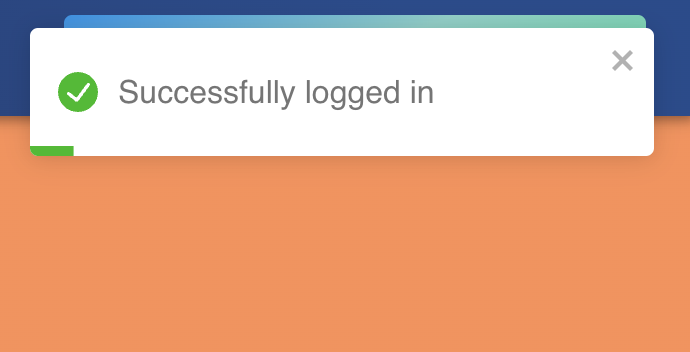
\includegraphics[width=4cm]{img/results/auth-success-notification.png}
\caption[Insurechain: Notification when login succeeds ]{\footnotesize{Notification when login succeeds.}}
\label{fig:auth-success-notification}
\end{figure}

Now, as is represented in figure \ref{fig:header-signed-in}, the header toolbar updates its layout in order to display the first and last characters of the account signed in. This is useful since a user may have several accounts.

\begin{figure}[H]
\centering

\includegraphics[width=12cm]{img/results/header-signedIn.png}
\caption[Insurechain: Header when user sign in succeeds ]{\footnotesize{Toolbar when user sign in succeeds.}}
\label{fig:header-signed-in}
\end{figure}

When clicking this new element, a modal appears to display some information retrieved from the connected wallet. In addition, a button to get disconnected when the user desires and another button to copy the full account address is rendered. You may find it in figure \ref{fig:signed-in-modal}.

\begin{figure}[H]
\centering
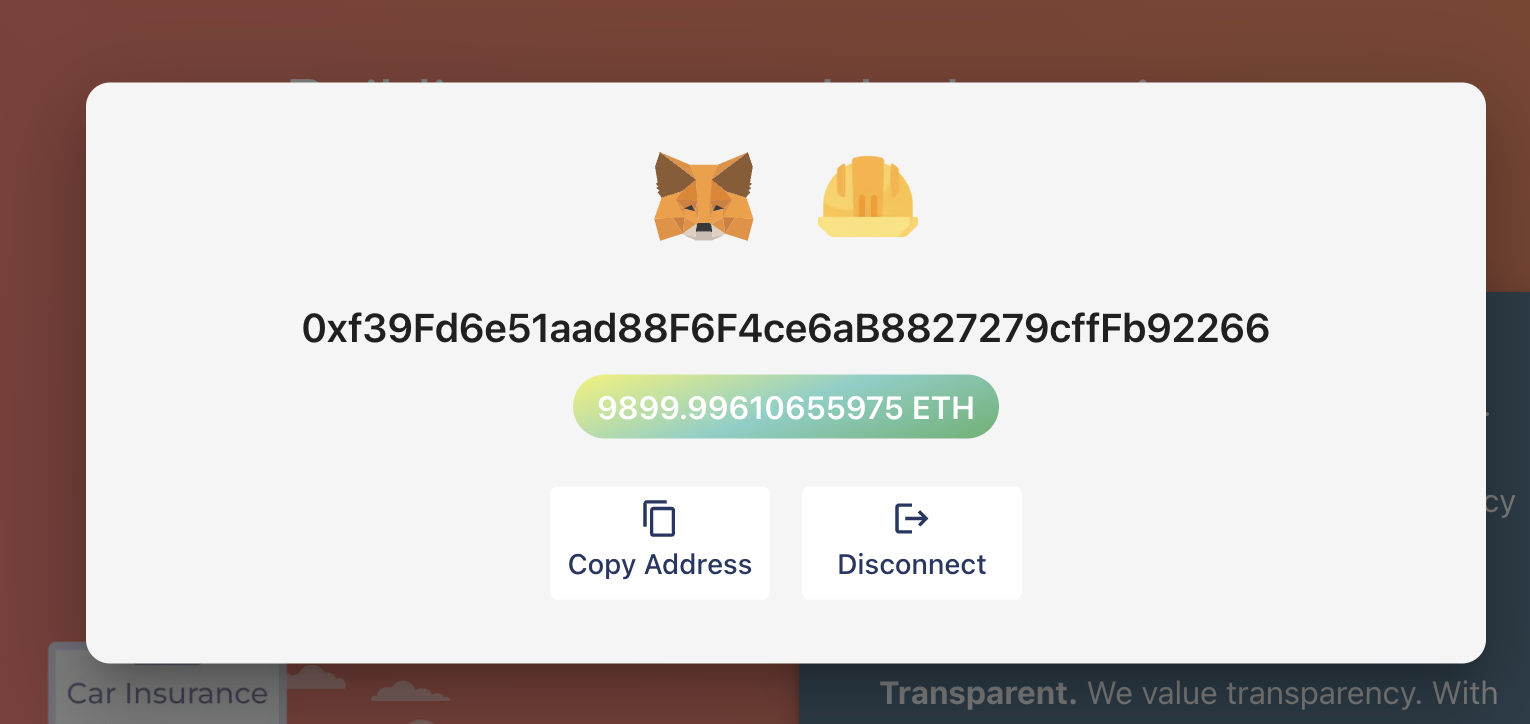
\includegraphics[width=6cm]{img/results/auth-signed-in-modal.png}
\caption[Insurechain: User account modal ]{\footnotesize{User account modal.}}
\label{fig:signed-in-modal}
\end{figure}
}

\subsubsection{Creating a proposal}
{
The user can access the signed-in or not to the insurance contraction page. There, he may find a first form where the user has to introduce all the data about the car to be covered as presented in figure \ref{fig:checkout-car-form}.

\begin{figure}[H]
\centering
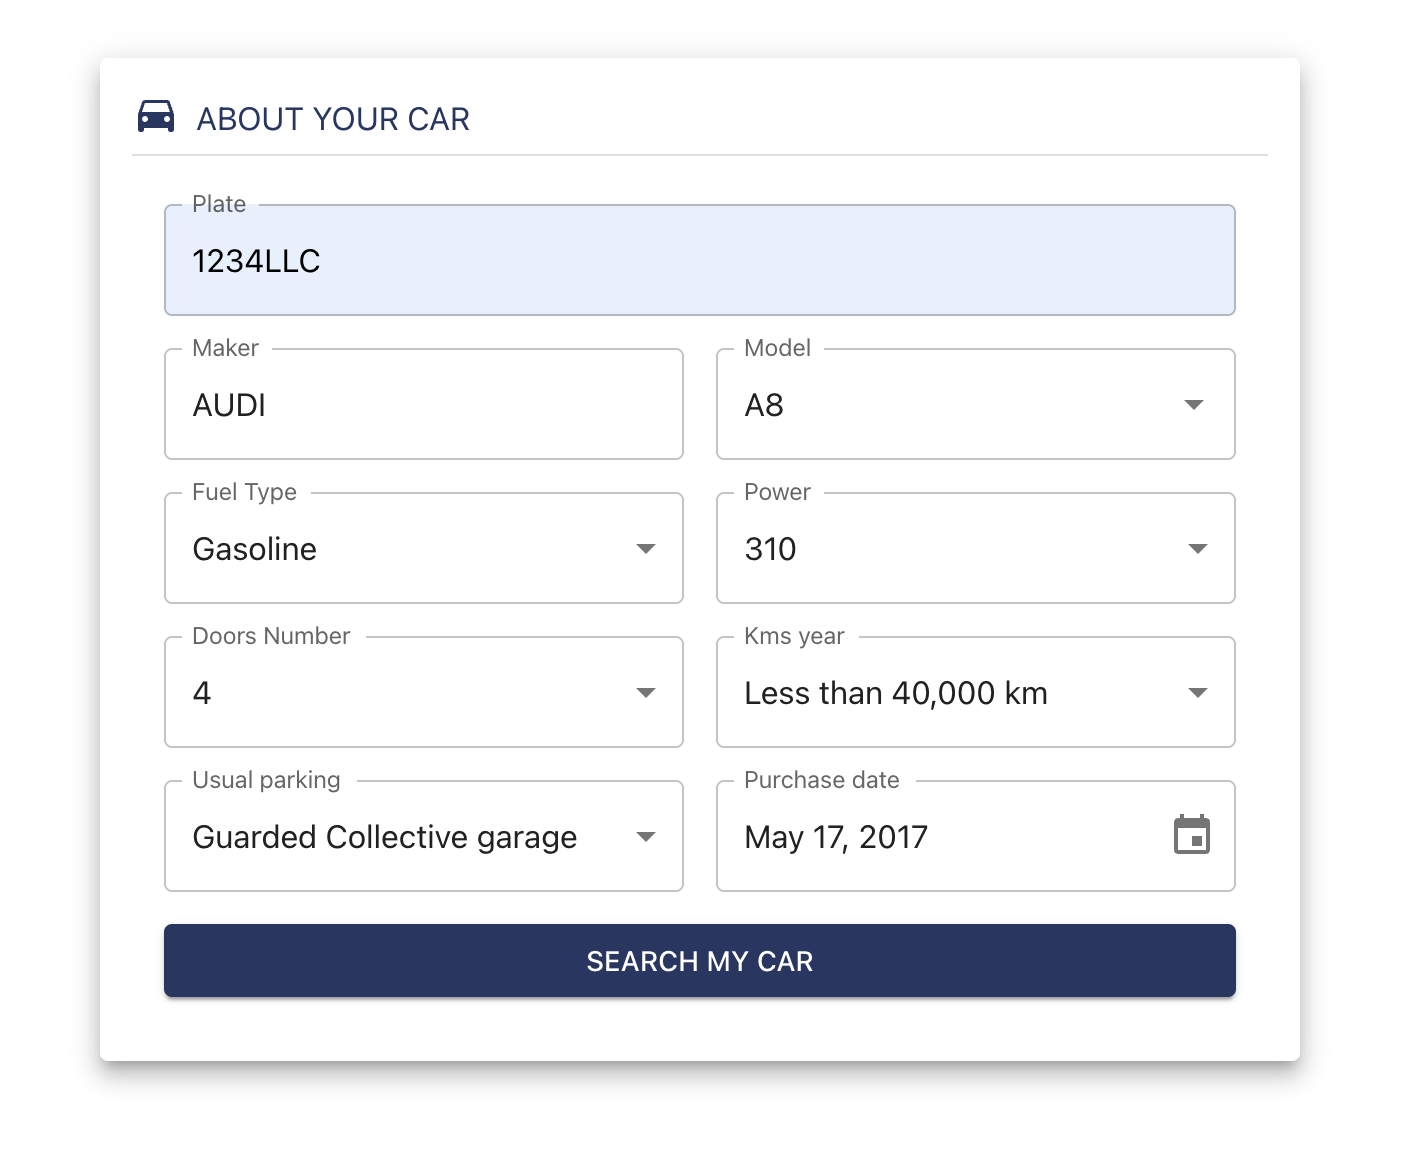
\includegraphics[width=10cm]{img/results/checkout-car.png}
\caption[Insurechain: Car form insurance enrollment]{\footnotesize{Car form insurance enrollment.}}
\label{fig:checkout-car-form}
\end{figure}
Then, the user must select the specific version for the car detailed as is demonstrated in figure \ref{fig:checkout-select-version}. These car models are consumed for a public API.

\begin{figure}[H]
\centering
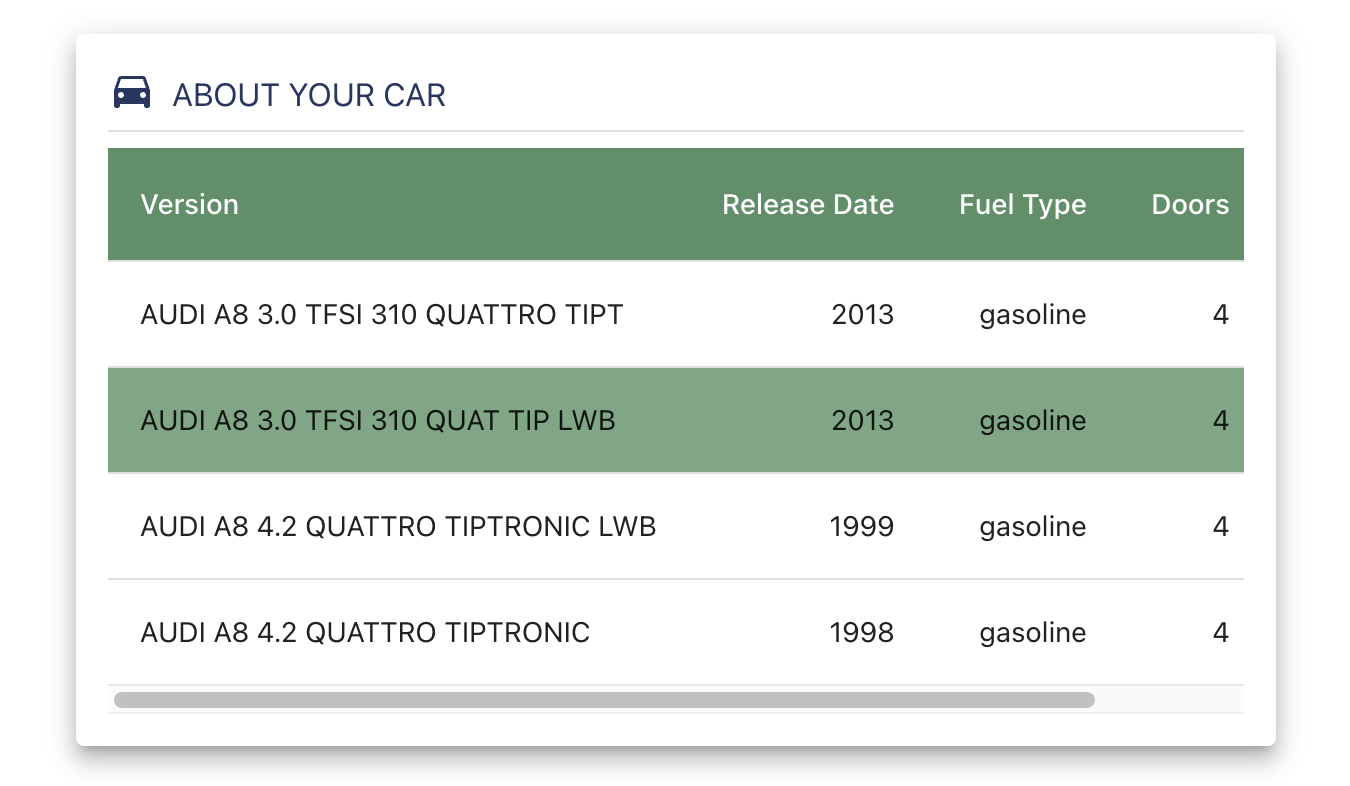
\includegraphics[width=10cm]{img/results/checkout-select-version.png}
\caption[Insurechain: Car version selection in insurance enrollment]{\footnotesize{Car version selection in insurance enrollment.}}
\label{fig:checkout-select-version}
\end{figure}

With the specific version and model of the car defined, the app displays a form to ask for the driver's information. Note in figure \ref{fig:checkout-driver-form} that the car information is collected and displayed in the first block above the driver's form.

\begin{figure}[H]
\centering
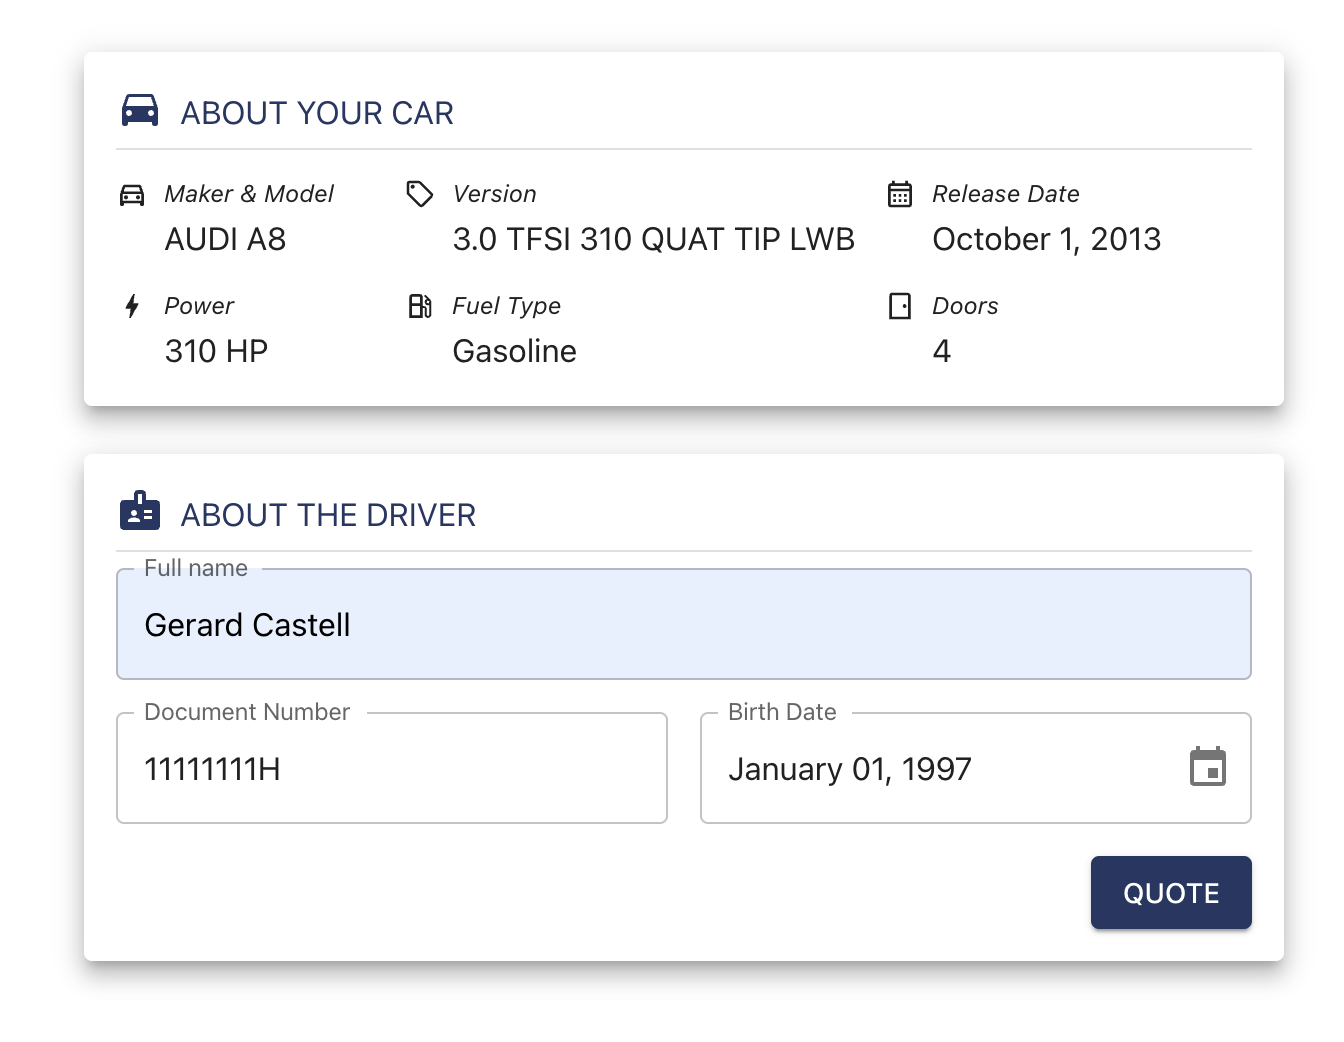
\includegraphics[width=10cm]{img/results/checkout-about-you.png}
\caption[Insurechain: Driver form in insurance enrollment]{\footnotesize{Driver form in insurance enrollment.}}
\label{fig:checkout-driver-form}
\end{figure}

With all this information introduced, a summary of such risk figures is displayed on top as shown in figure \ref{fig:checkout-coverage-selection}, the web app makes a quote and the backend calculates a price for each coverage type. This price is random since it is out of the scope of the project. Thus, the backend server returns all the coverage products with a monthly price associated and the web displays it. Note that the price is reflected in euros and \acrshort{eth}. This conversion is obtained in real time to a public API.

\begin{figure}[H]
\centering
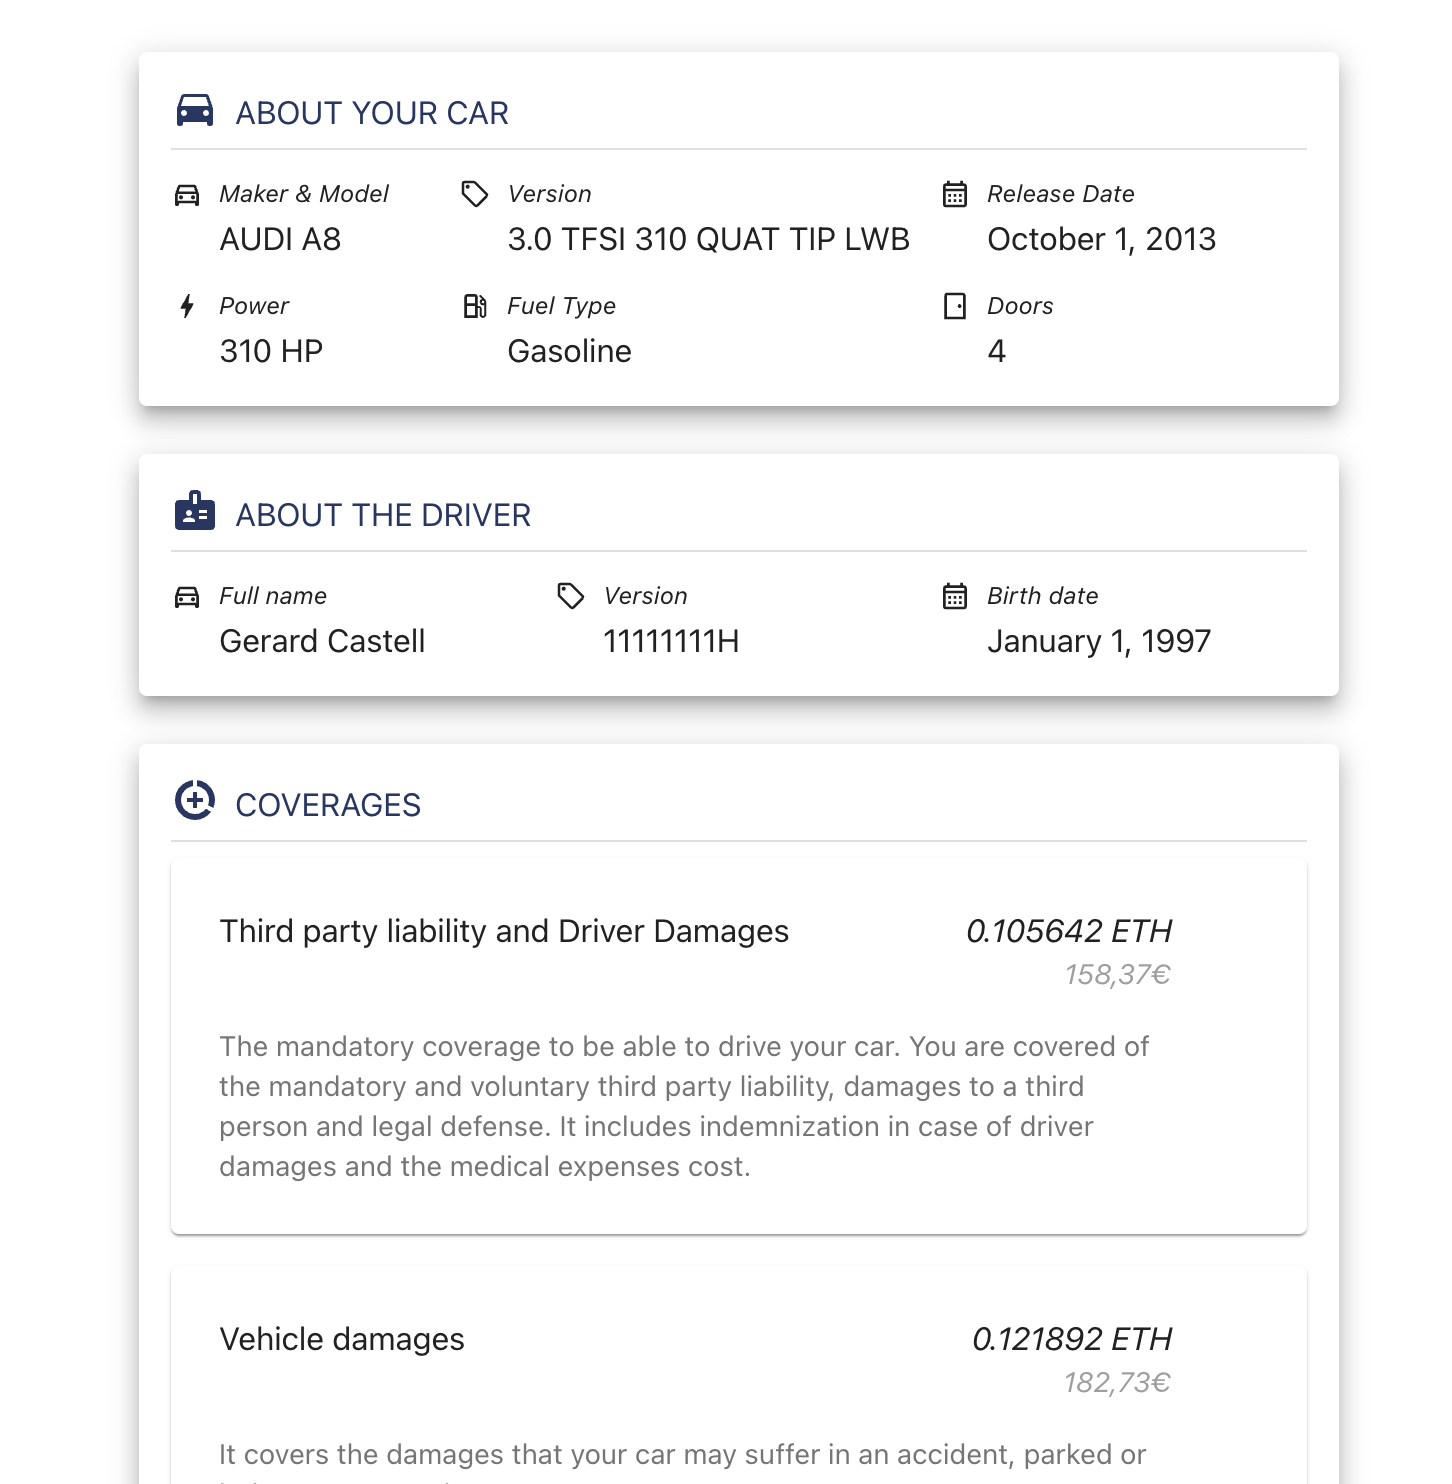
\includegraphics[width=10cm]{img/results/checkout-coverage-selection.png}
\caption[Insurechain: Risk figures summary in insurance enrollment]{\footnotesize{Risk figures summary in insurance enrollment.}}
\label{fig:checkout-coverage-selection}
\end{figure}

The user can select the coverage types in which he is interested and then save the proposal when he is ready as illustrated in figure \ref{fig:checkout-coverage-selection-2}.

\begin{figure}[H]
\centering
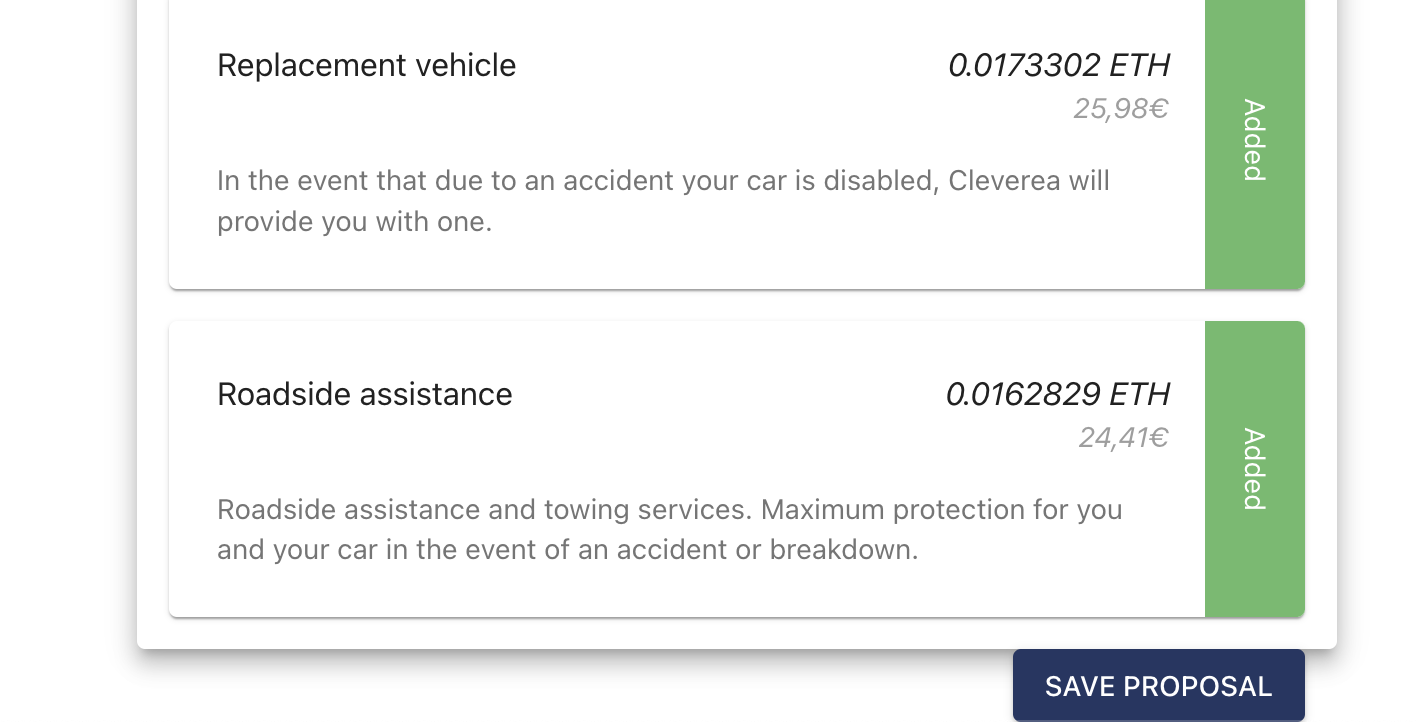
\includegraphics[width=10cm]{img/results/checkout-coverage-selection-2.png}
\caption[Insurechain: Coverage types selection in insurance enrollment]{\footnotesize{Coverage types selection in insurance enrollment.}}
\label{fig:checkout-coverage-selection-2}
\end{figure}

Eventually, when the user wants to confirm it has to be signed in. Otherwise, a modal like the one in figure \ref{fig:metamask-sign-in} will appear. Once logged in, the web app sends the proposal configuration with the risk figures data to the backend with the authentication header. The backend stores the proposal bound to that client in the database and returns an OK. Consequently, the web displays a modal announcing the confirmation as you can see in figure \ref{fig:checkout-succeed-modal}.

\begin{figure}[H]
\centering
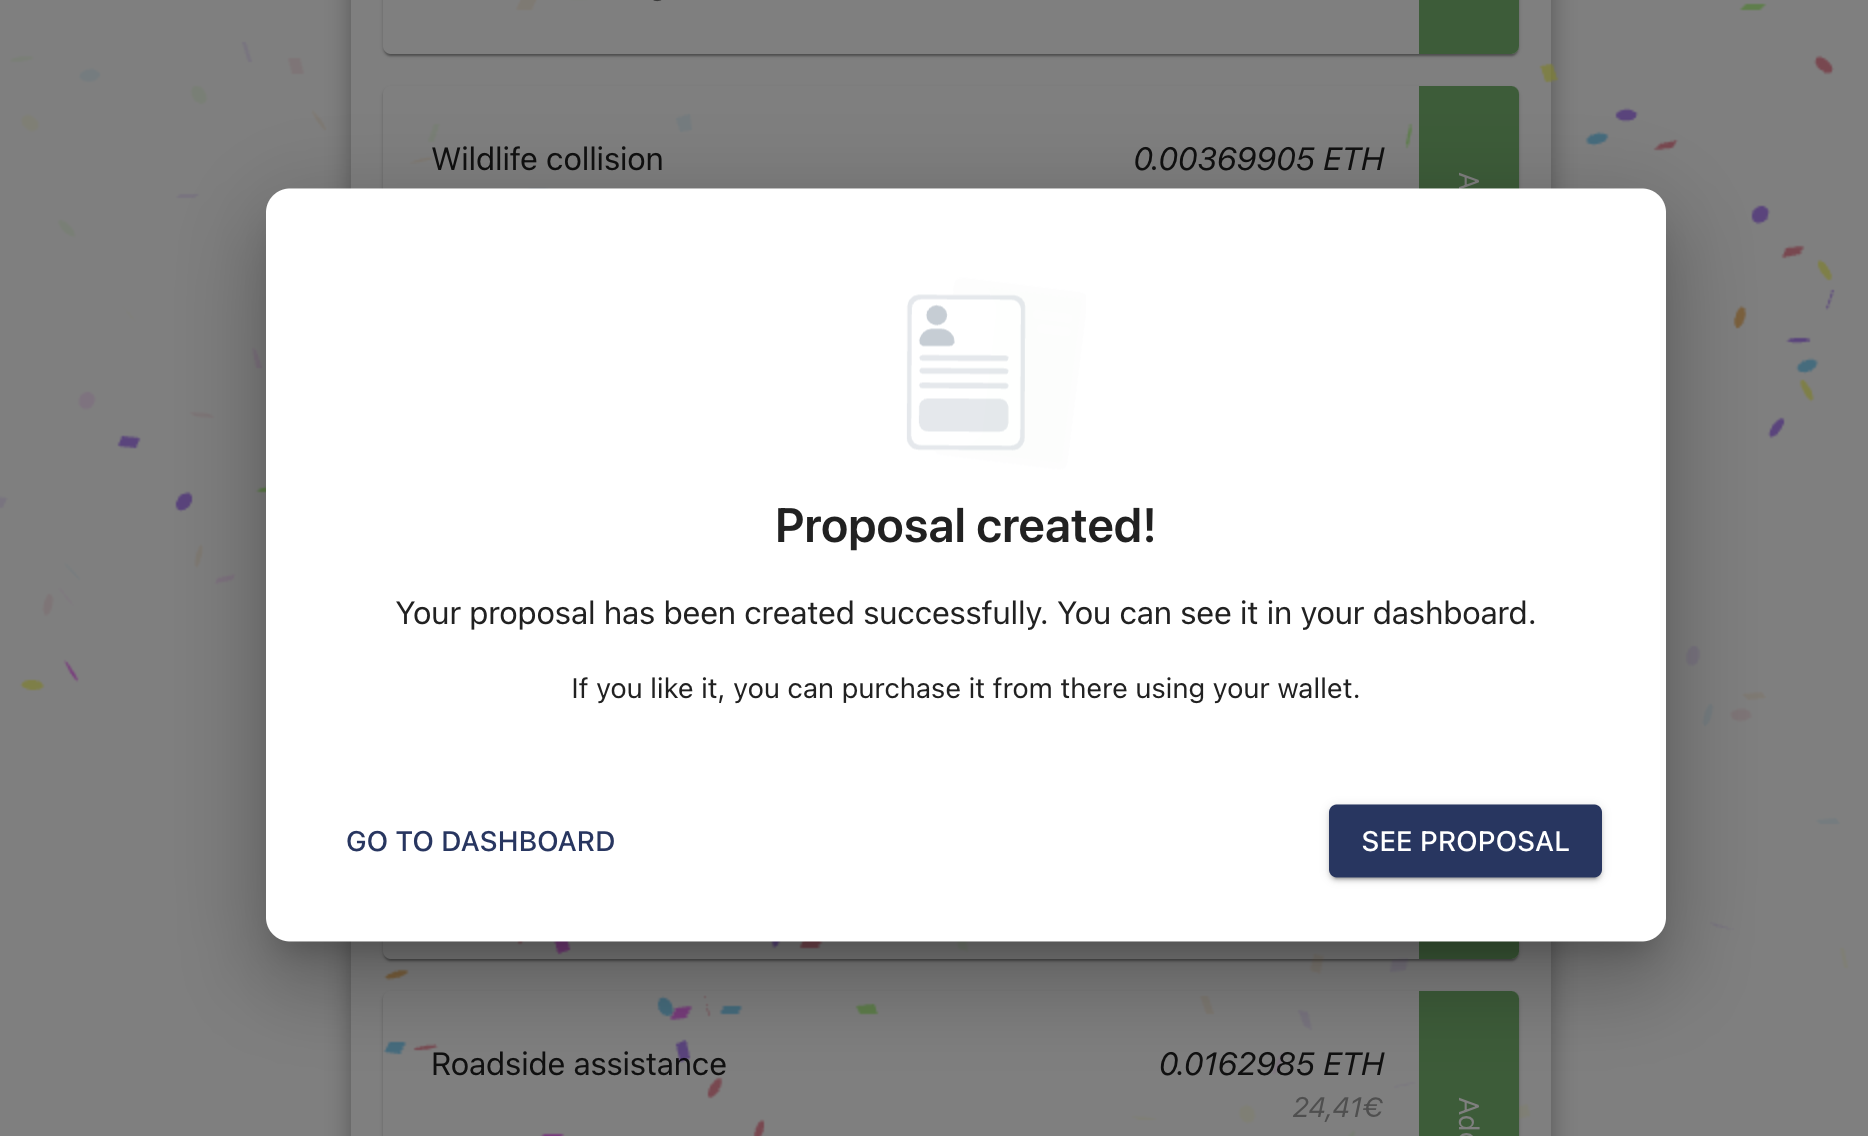
\includegraphics[width=10cm]{img/results/checkout-succeed.png}
\caption[Insurechain: Succeed modal in insurance enrollment]{\footnotesize{Succeed modal in insurance enrollment.}}
\label{fig:checkout-succeed-modal}
\end{figure}
}

\subsubsection{Show user proposals}
{
If the user wants to see their proposals he can access them on the dashboard page, where he may find two boxes to visit existing proposals or policies as revealed in figure \ref{fig:dashboard-page}.

\begin{figure}[H]
\centering

\includegraphics[width=8cm]{img/results/dashboard.png}
\caption[Insurechain: Dashboard page]{\footnotesize{Dashboard page.}}
\label{fig:dashboard-page}
\end{figure}

If the user selects proposals, the user proposals page will appear as in the figure \ref{fig:proposals-page}.
On this page, the user may find all his proposals, purchased and still not, listed with a summary of this accorded data and price.

\begin{figure}[H]
\centering
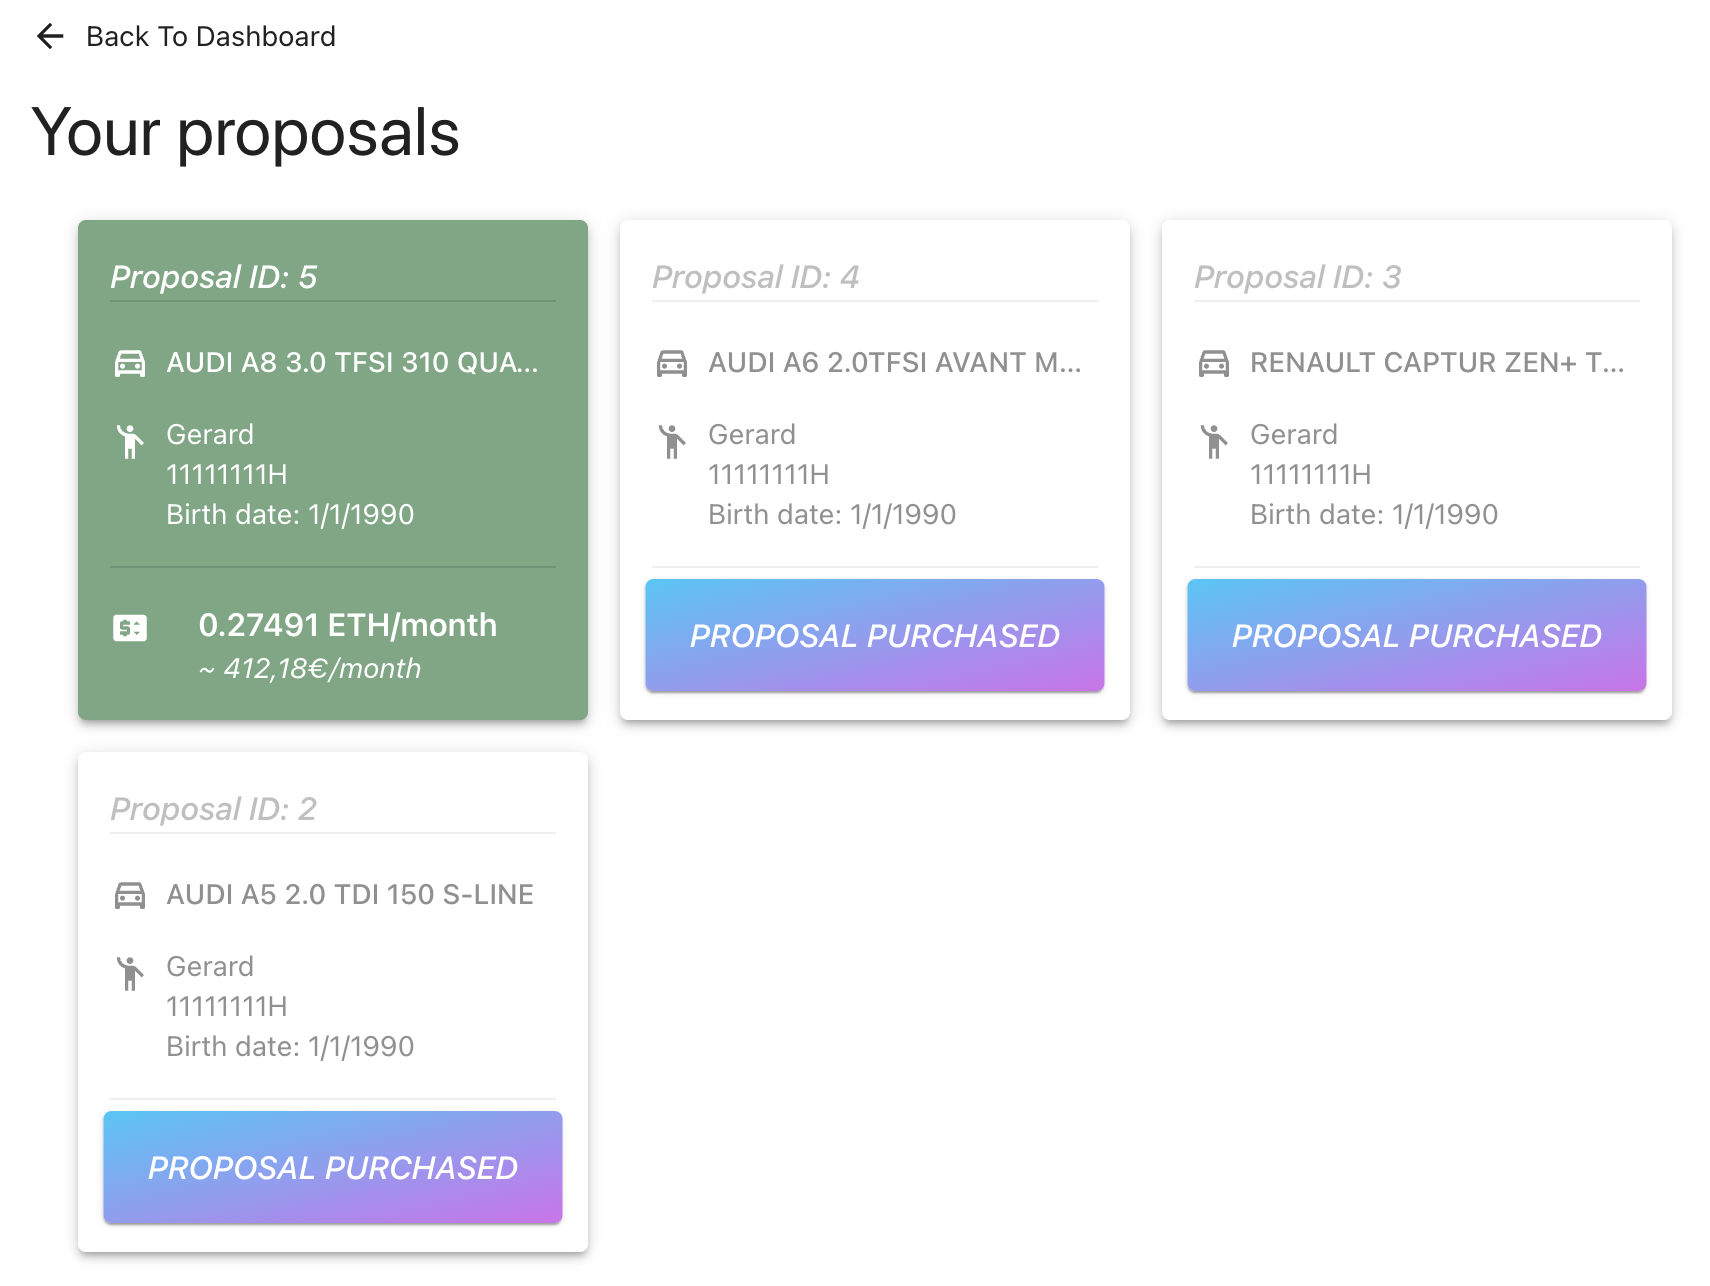
\includegraphics[width=12cm]{img/results/proposals-list.png}
\caption[Insurechain: Proposals page]{\footnotesize{Proposals page.}}
\label{fig:proposals-page}
\end{figure}

If the user selects the first one which is the last one created he will navigate to the detail of such proposal as reflected in figure \ref{fig:proposal-detail}.
\begin{figure}[H]
\centering
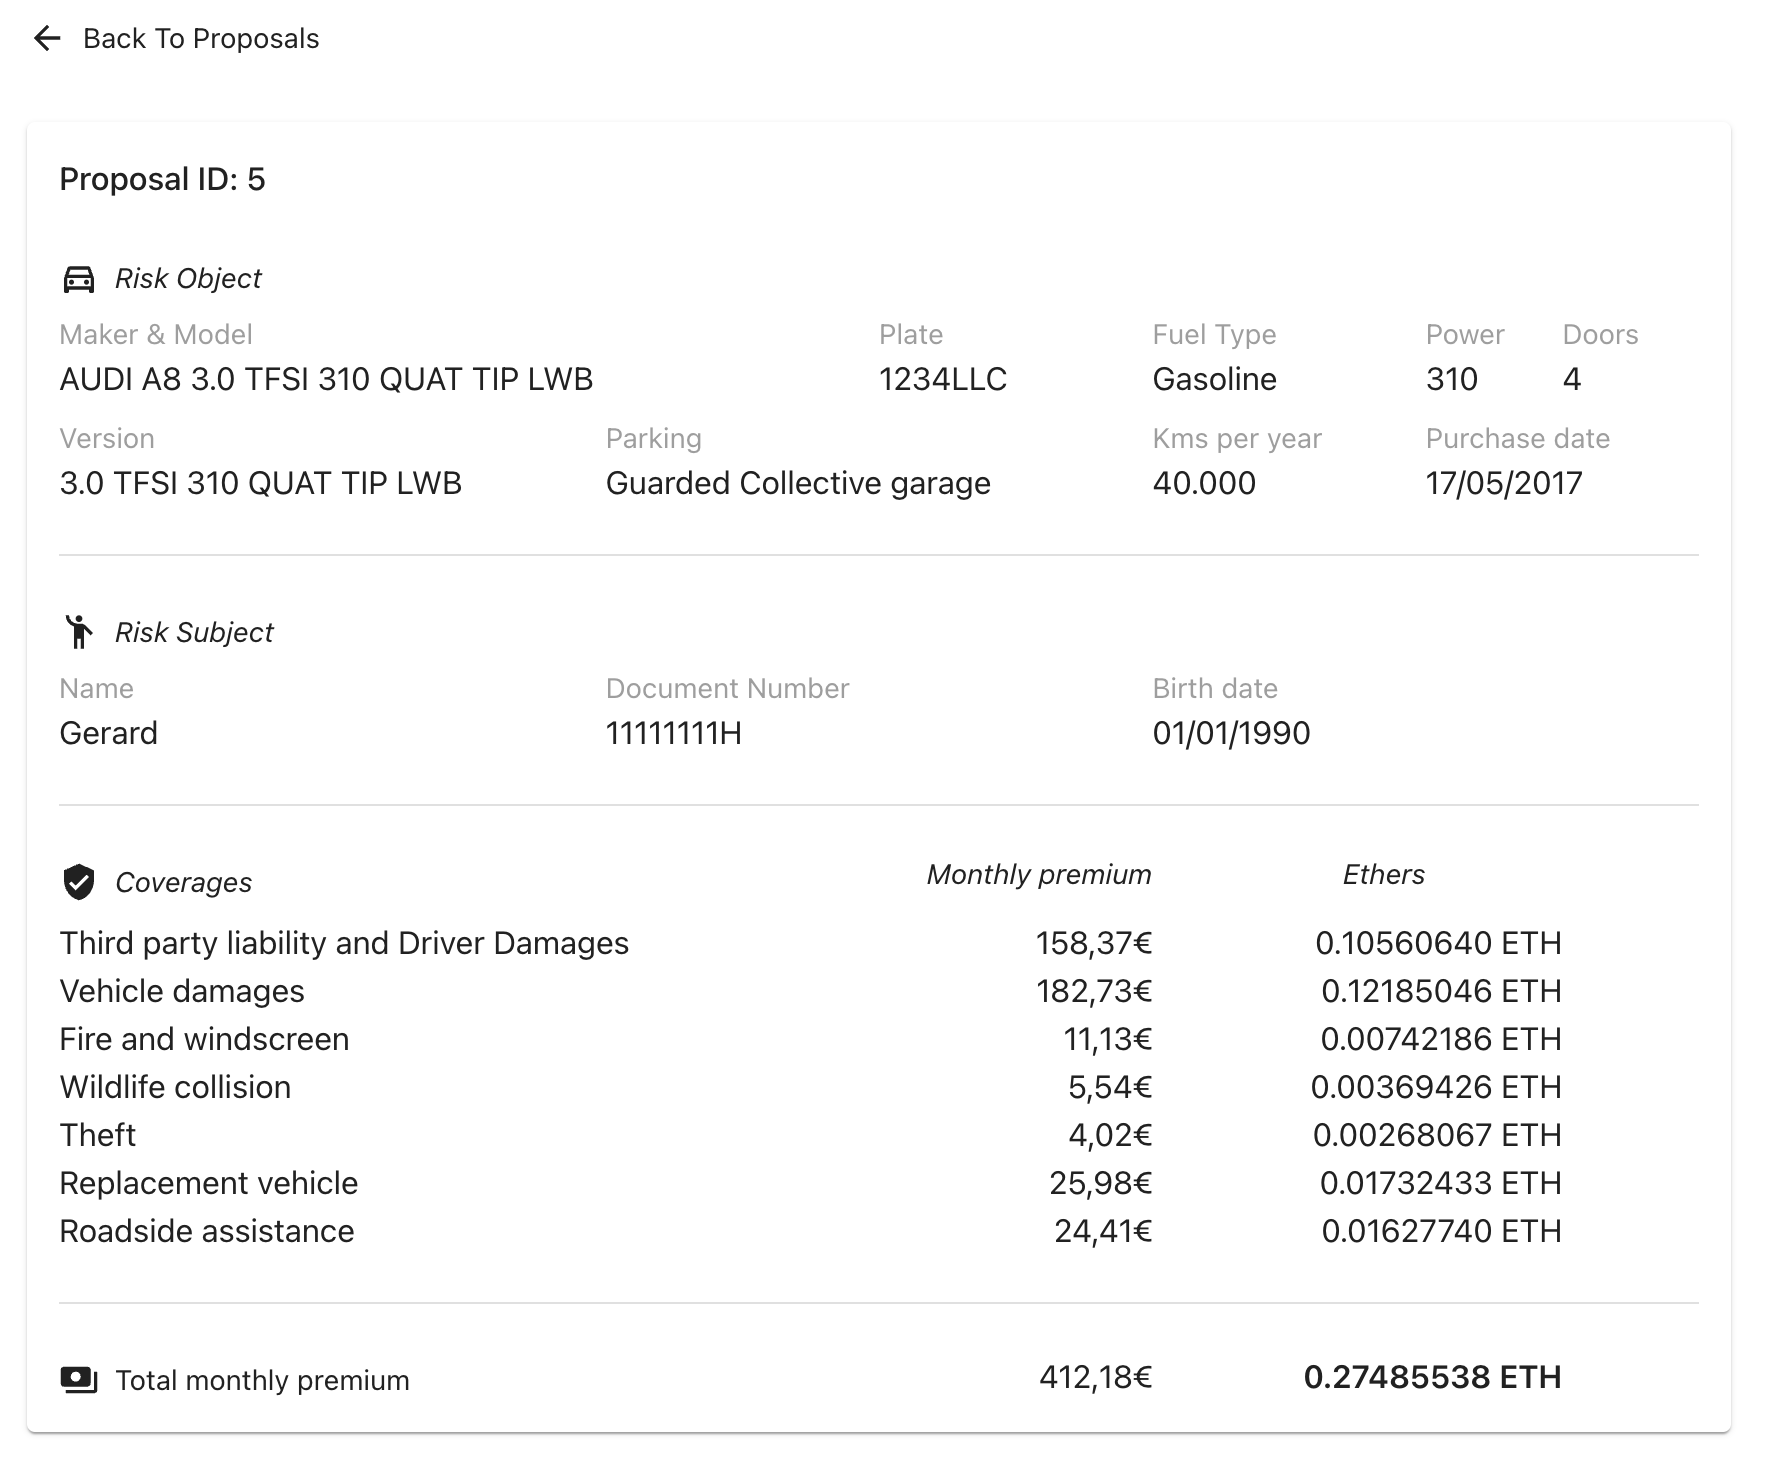
\includegraphics[width=12cm]{img/results/proposal-detail-1.png}
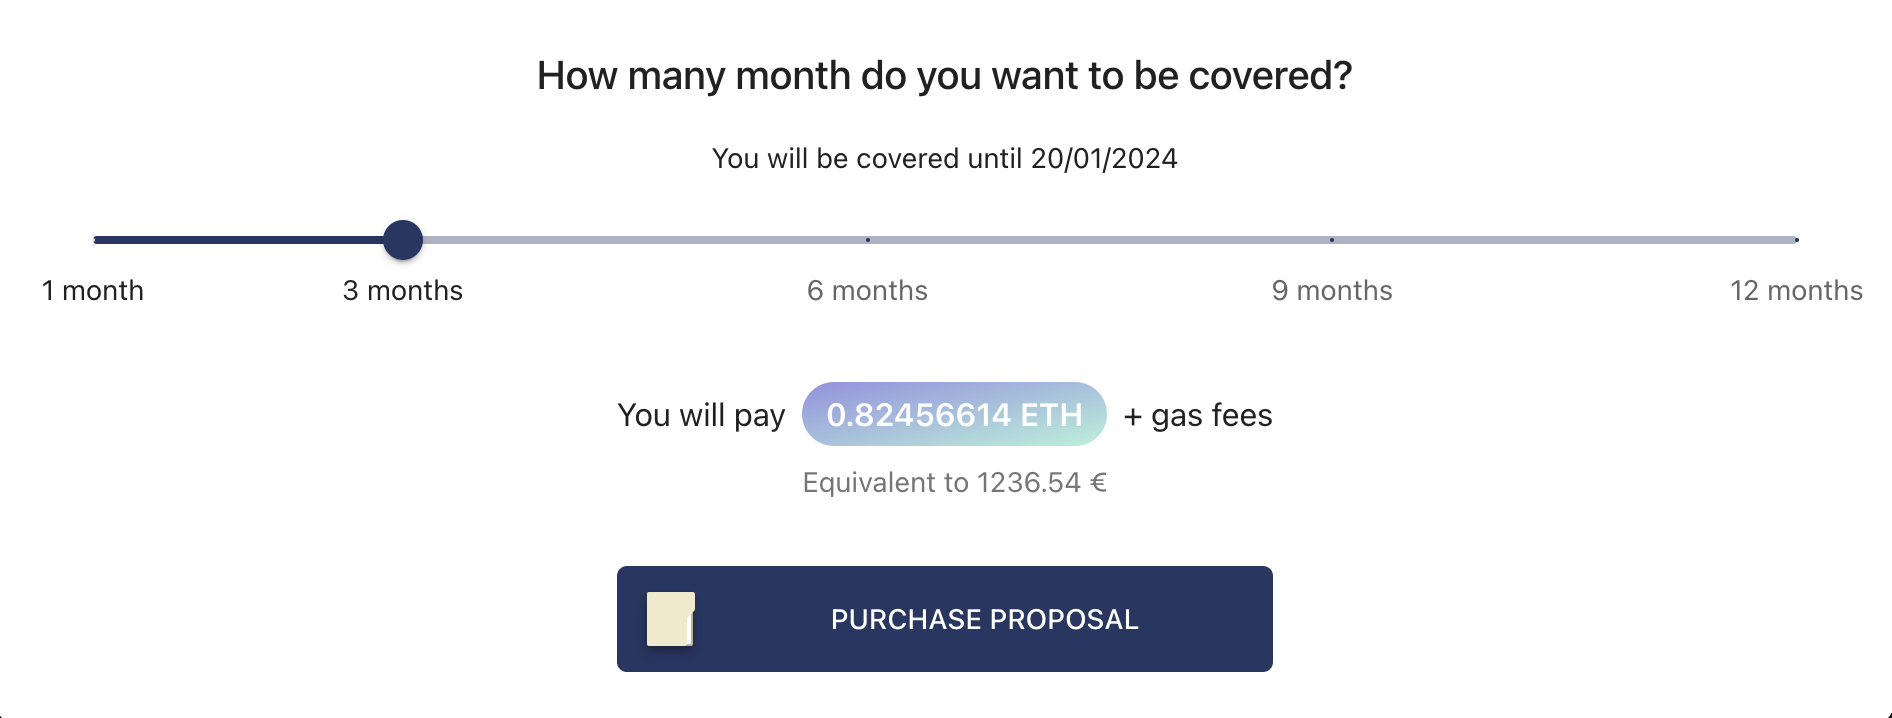
\includegraphics[width=12cm]{img/results/proposal-detail-2.png}
\caption[Insurechain: Proposal detail page]{\footnotesize{Proposal detail page.}}
\label{fig:proposal-detail}
\end{figure}

The web requests the backend for the specific proposal and it is returned. Then the user may find on this page all the proposal information collected on the proposal form. It is important to focus that for purchase the user must select the number of months to be covered from the current day. The total monthly amount will be multiplied by the number of months and this total price is indicated at the bottom. Take into account that this is a rough calculation because the \acrshort{eth} cannot be accurate at that moment and the gas needed to purchase the policy is not estimated.
}

\subsubsection{Purchase proposal}
\label{section:purchase-proposal}
{
In the proposal detail page, when the user clicks the purchase proposal button the wallet will display a confirmation of the according transaction as shown in figure \ref{fig:purchase-transaction}.

\begin{figure}[H]
\centering
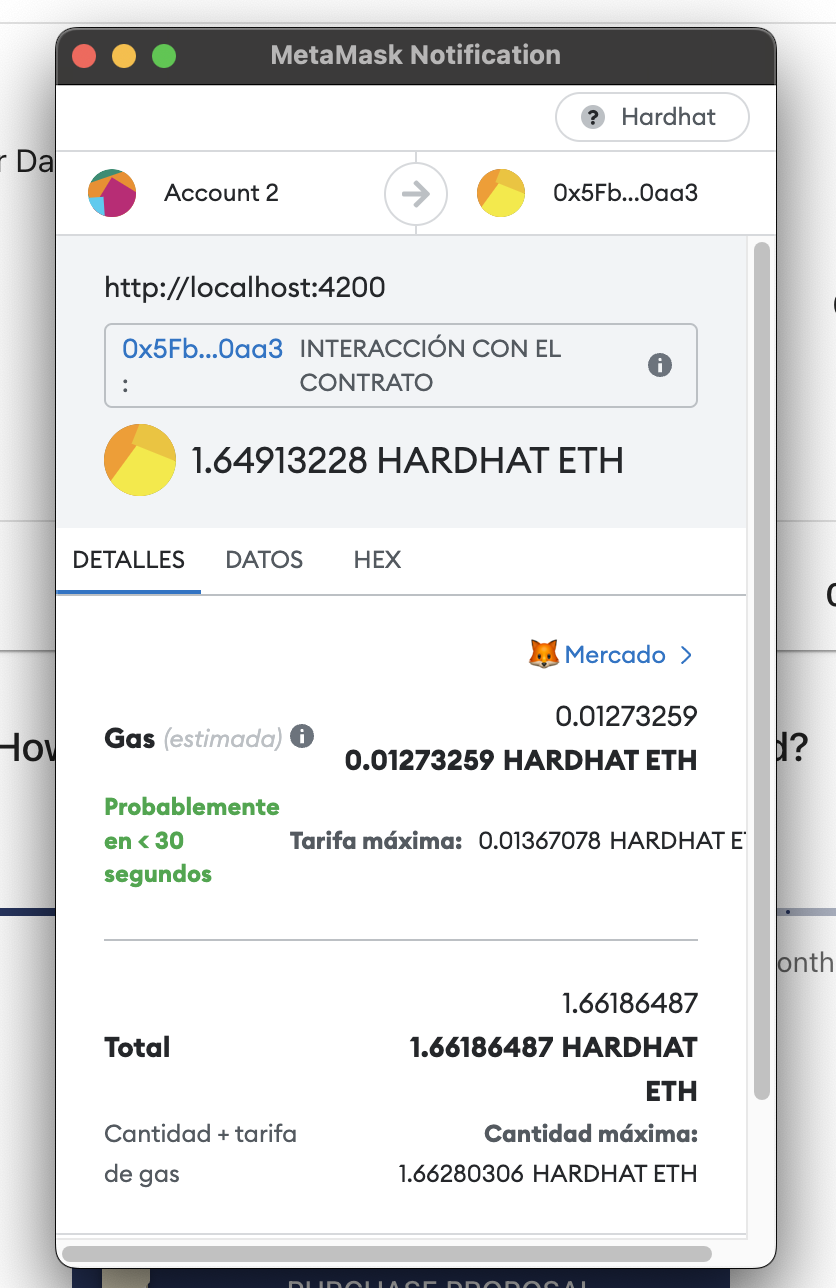
\includegraphics[width=6cm]{img/results/purchase-transaction.png}
\caption[Insurechain: Purchase transaction]{\footnotesize{Purchase transaction.}}
\label{fig:purchase-transaction}
\end{figure}


If the user agrees, the transaction will be sent to the factory smart contracts. If the computation succeeds a modal will be displayed as you may see in figure \ref{fig:purchase-succeed-modal}. 

\begin{figure}[H]
\centering
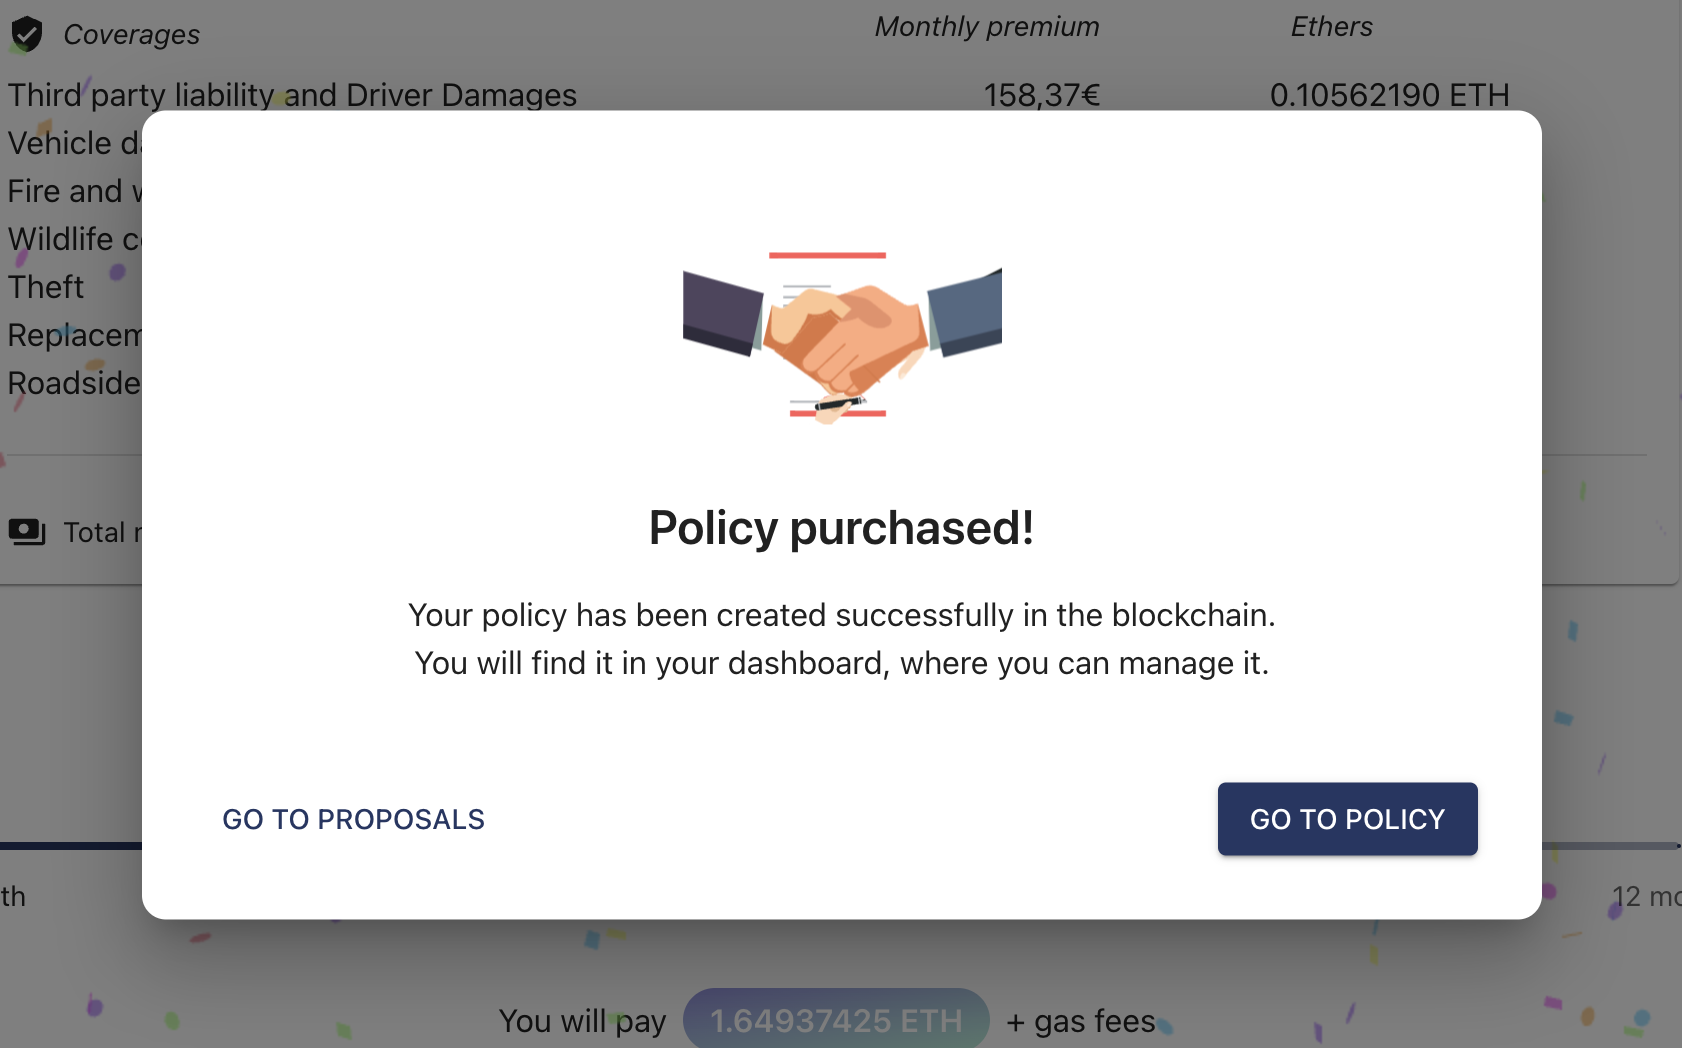
\includegraphics[width=10cm]{img/results/purchase-succeed-modal.png}
\caption[Insurechain: Purchase succeed modal]{\footnotesize{Purchase succeed modal.}}
\label{fig:purchase-succeed-modal}
\end{figure}
Keep in mind, that the transaction has proceeded successfully, however, to consider the transaction as confirmed and make sure the data can be considered immutable in the Ethereum blockchain we must way a few blocks yet. If we evaluate the Metamask within that period of time we will see something similar to the figure \ref{fig:pending-transaction}.

\begin{figure}[H]
\centering
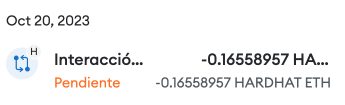
\includegraphics[width=6cm]{img/results/transaction-pending.png}
\caption[Insurechain: Transaction pending]{\footnotesize{Transaction pending.}}
\label{fig:pending-transaction}
\end{figure}
Eventually, when the wallet considers that enough blocks have been mined and the state is immutable the transaction turns confirmed as you can see in figure \ref{fig:confirmed-transaction}.

\begin{figure}[H]
\centering
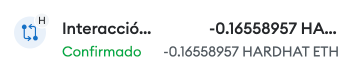
\includegraphics[width=6cm]{img/results/transaction-confirmed.png}
\caption[Insurechain: Transaction confirmed]{\footnotesize{Transaction confirmed.}}
\label{fig:confirmed-transaction}
\end{figure}
}

\subsubsection{Show user policies}
{
The user will find all the policies purchased and canceled on the policies page as illustrated in figure \ref{fig:policies-page}.

\begin{figure}[H]
\centering
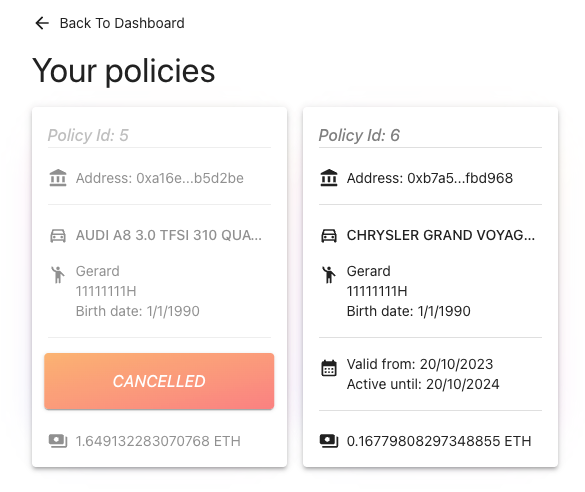
\includegraphics[width=8cm]{img/results/policies-page.png}
\caption[Insurechain: Policies page]{\footnotesize{Policies page.}}
\label{fig:policies-page}
\end{figure}

If we visit the policy purchased before, we have to see exactly the same data that was reflected in the proposal page but with the difference that now the source is the Policy smart contract deployed in the purchase and not the backend database. The total amount paid must be different because the price displayed is precisely the paid in the purchase transaction that was stored in the policy smart contract. This data comparison can be performed by comparing figures \ref{fig:proposal-detail} and \ref{fig:policy-detail}.

\begin{figure}[H]
\centering
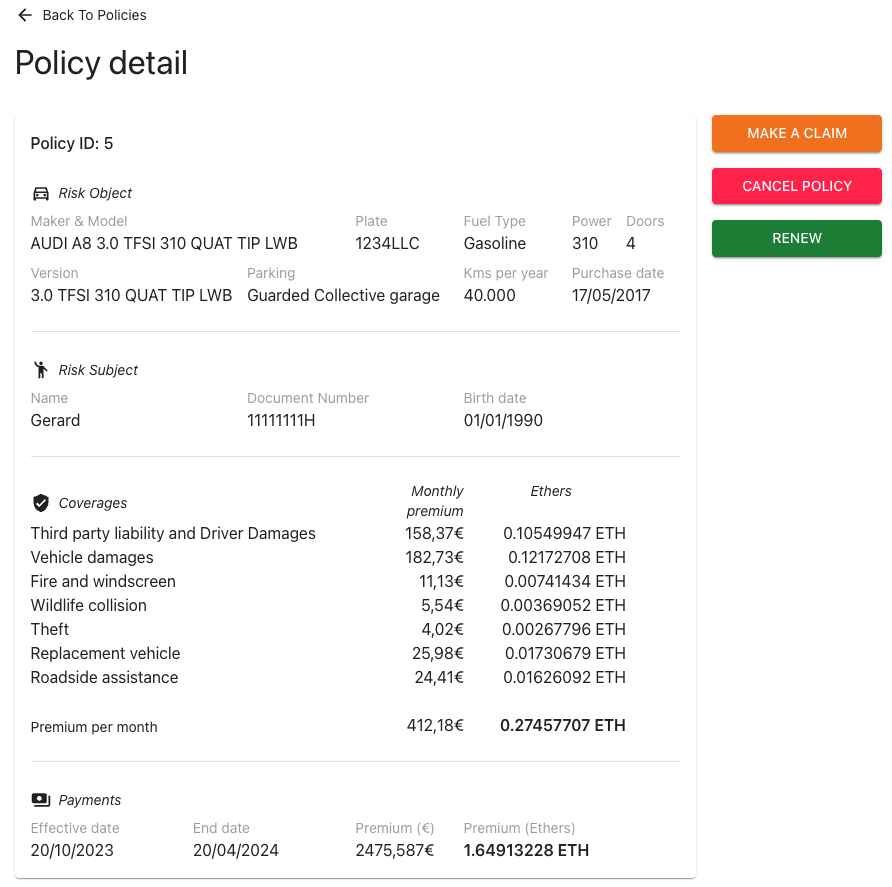
\includegraphics[width=12cm]{img/results/policy-detail.png}
\caption[Insurechain: Policy detail page]{\footnotesize{Policy detail page.}}
\label{fig:policy-detail}
\end{figure}

}

\subsubsection{Cancel policy}
{
Furthermore, if we look at the right side we find three buttons to make a claim, renew and cancel. Just the cancel button is implemented as explained before. If we press this button, the web app estimates how much \acrshort{eth} would be refunded to the user according to the time not consumed of the policy live as observed in the figure \ref{fig:cancel-modal}.

\begin{figure}[H]
\centering
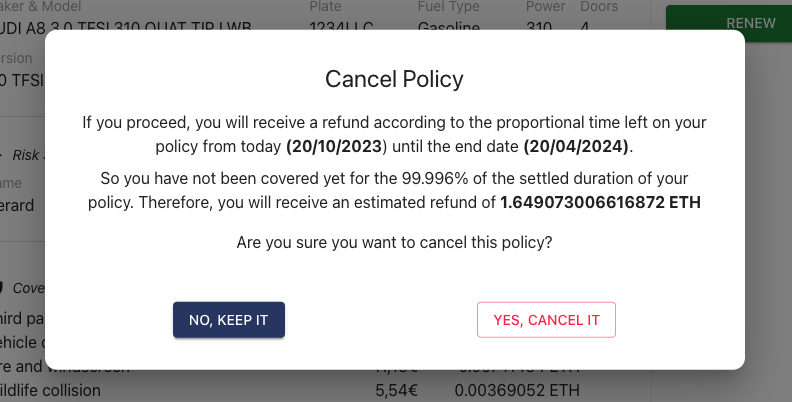
\includegraphics[width=9cm]{img/results/cancel-modal.png}
\caption[Insurechain: Cancel policy prompt modal]{\footnotesize{Cancel policy prompt modal.}}
\label{fig:cancel-modal}
\end{figure}

If the user confirms the modal, the wallet will trigger a transaction modal to confirm the gas spent as you may see in figure \ref{fig:cancel-transaction}. This is due to the user is going to modify the state of the policy contract since some store variables are going to change their value such as the end date or the renewal date. The amount of \acrshort{eth} is not too high so it is reasonable that this charge falls on the client side.

\begin{figure}[H]
\centering
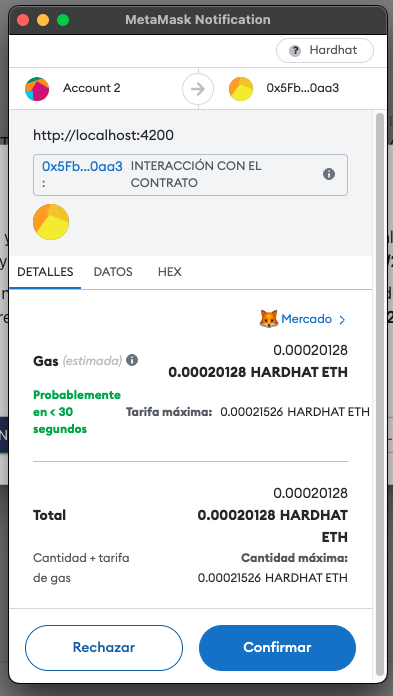
\includegraphics[width=6cm]{img/results/cancel-transaction.png}
\caption[Insurechain: Cancel policy transaction]{\footnotesize{Cancel policy transaction.}}
\label{fig:cancel-transaction}
\end{figure}

When the user confirms the transaction if the operation succeeds the user will see the layout displayed in figure \ref{fig:policy-canceled}. Even though, as explained in the section \ref{section:purchase-proposal} the operation has succeeded, nevertheless, to consider the state immutable we must wait for a few transactions.

\begin{figure}[H]
\centering
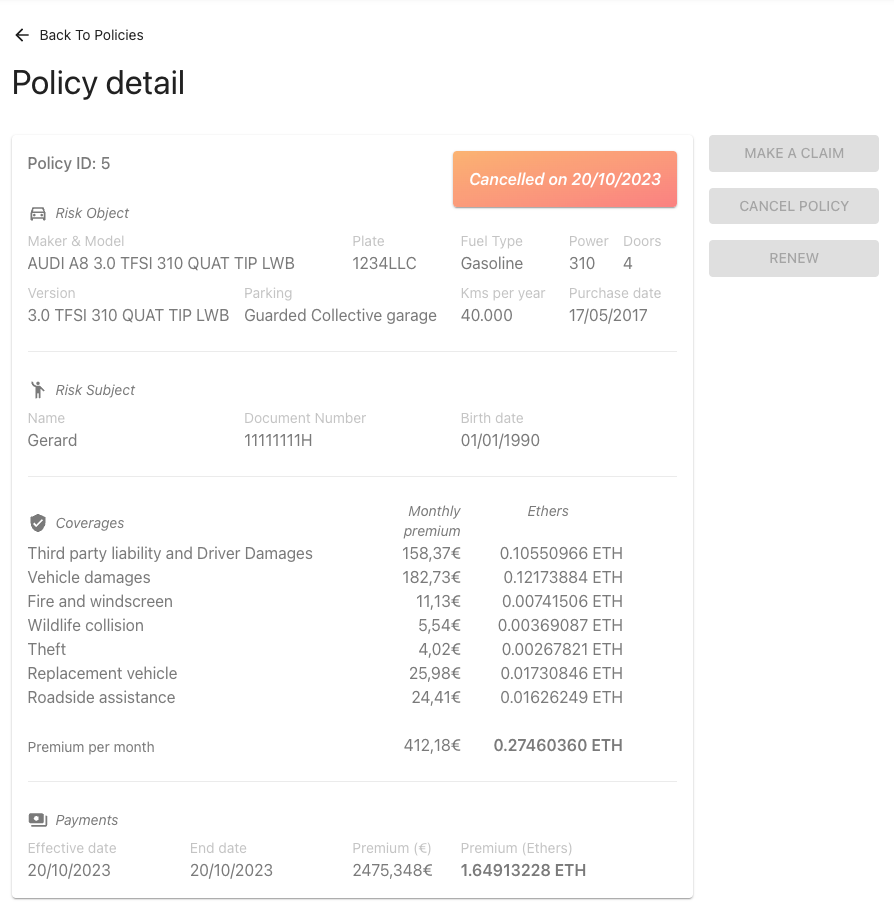
\includegraphics[width=10cm]{img/results/policy-canceled.png}
\caption[Insurechain: Policy canceled page]{\footnotesize{Policy canceled page.}}
\label{fig:policy-canceled}
\end{figure}
}

%%% BUDGET %%%
\clearpage

\section{Budget}
{\selectlanguage{english}
\foreignlanguage{english}{
The whole experiment has been carried out with free open source. In addition, I just needed a computer to run all the pieces locally and no more infrastructure was required. Therefore, the experiment was quite cheap.

Nevertheless, we can assume this proof of concept is performed by a company and estimate the budget. To do so, we will have to buy the computer and pay the salary of the developer and training resources. 

On the one hand, the computer could be anyone with proper power which is valued at around \textbf{\euro{800}} with taxes included. On the other hand, the time spent on developing the experiment is around 600 hours in my case, 30 weeks working 20 hours per week. Moreover, we may assume a net salary for a full stack average developer of around \euro{15} per hour. Taking into account that the 30\% is subject to the IRPF tax, to maintain such a net salary we need to pay a gross salary of \euro{21.42} per hour. In conclusion, if we multiply the 600 hours of work by the \euro{21.42} per hour we obtain then the total salary sums up to \textbf{\euro{12857.15}}. Finally, the training to learn how to develop smart contracts and an off-blockchain backend has a price of \textbf{\euro{40}} altogether. The table \ref{tab:budget} collects all the expenses aforementioned.

\begin{table}[h!]
\centering
\caption[Budget]{ \footnotesize This table gathers the different concepts that a company should pay to carry out the project as a proof of concept}
\label{tab:budget}
\footnotesize{
\begin{tabular}{||c c ||} 
 \hline
 Concepts & Cost \\ [0.5ex] 
 \hline\hline
  Computer & \euro{800}  \\
 Wage & \euro{12857.15} \\ 
 Training & \euro{40}  \\ [1ex] 
 \hline
 Total & \euro{13697.15} \\ [0.5ex] 
 \hline
\end{tabular}
}
\end{table}

}
}

%%% ENVIRONMENT %%%
\clearpage

\section{Environment Impact}
{
The Ethereum consensus was previously based on \acrlong{pow}, which mining process consumes a significant amount of energy to resolve the complex cryptographic puzzle. 

Ethereum was concerned about this issue and migrated to \acrlong{pos} consensus finishing in September 2022, which drastically reduced the energy consumption since now miners do not race to find the hash. The energy used for \acrshort{pos} depends on the sources so it has even less carbon footprint if it comes from renewable energy sources.

The environmental impact of the Ethereum blockchain versus a traditional backend with a database model depends on various factors but are quite similar models in terms of energy consumption and possible solutions. The transition to PoS and the use of renewable energy sources are positive steps for reducing the environmental footprint of blockchain technology. However, it is essential to consider efficiency, scaling, and the energy mix to assess the overall impact accurately.
}

%%% CONCLUSION AND FUTURE %%%
\clearpage
\section{Conclusions and future development }

{
In this thesis, I have converted a traditional insurance model to a blockchain-based approach from end to end. The experiment is considered successful since the resulting dapp gathers all the pieces needed to offer a realistic digital product. These pieces include a frontend web application to provide access to the dapp for the users, a traditional backend server and database to generate and store the policy proposals, and eventually several smart contracts in charge of managing the core business logic.

It is been really gratifying to have developed the entire software with technology ahead of the curve, which has given me a wide knowledge about how to build an MVP of a product, taking always into account the user as the focus of the product. It is been a very large project but without any doubt, I have enjoyed every line of code I have written.

About blockchain technology, I have to admit that the more I read about it the more impressed I was. To figure out how transactions can be programmable brings to my mind a lot of business cases to apply in which all parties involved would benefit from. It truly represents a game changer in a moment where the big companies have our data ownership completely. Without any doubt, I would love to see how companies start migrating toward Web 3.0 models where all transactions and data live in a more secure, traceable and censorship-resistance ecosystem. However, it represents a huge technical investment that without representing a clear benefit for companies I do not believe that they will carry out.

Moreover, it is very satisfactory to know that this exact dapp could be deployed in a real-world scenario without a few modifications. Even though, if I get realistic I consider most end-users might find to understand the Ethereum basis and use this kind of tool that really leverages blockchain power cumbersome. In favor of reducing this effect, software solutions built on top of the Ethereum layer, such as browser wallets like Metamask, are appearing in order to make it more accessible and understandable. Nevertheless, the migration of the Web 2.0 models towards blockchain-based solutions will have to happen slowly and incrementally, trusting part of the logic and data managed in centralized services taking care of not eliminating the benefits of blockchain. It is a good example of this the off-blockchain server that generates and stores proposals in the experiment which is forced to exist in order to not differ too much from the original insurance business model.

From my point of view, we are still far from using daily dapps for our regular tasks but as technology advances, it may represent at some point a crucial player to take advantage of. In the same way that large-language models have nowadays exploded in popularity and demand and most companies are trying to include them in their stack to improve their product value, perhaps at some point, blockchain will be the key to offering these valuable solutions too. 

In brief, we cannot force users to use a specific technology but that technology must offer a solution to the users in order to be used.

}

%%% GLOSSARY %%%
\clearpage
\printglossary

%%% BIBLIOGRAPHY %%%
\newpage

\medskip
\bibliographystyle{unsrt}
\bibliography{bibliography.bib}

%%% ANNEX %%%
\clearpage
\newpage

\begin{appendices}

\section{Deployment scenarios for a dapp}
\label{appendix:deployment-dapp}
{
{The hardware required to deploy the dapp depends on the use of it, so we can draw two scenarios:}
\begin{itemize}
    \item Development scenario. This case is used by developers to implement the software features before releasing it to a real scenario, well-known as Production. In this scenario, we just want to try the code locally and we do not need to make it public and accessible through the Internet for other users but us. This is the cheapest use case due to we can locally serve all the content on our computer. Assigning a different port for each process we can simulate a network where all the requests and communications happen through the different protocols like a real case would do. Both frontend and backend frameworks offer scripts out of the box to serve it locally. About the blockchain, we can simulate a local Ethereum network thanks to the Hardhat tool \cite{hardhat_network}. This tool emulates and hosts a real configurable network and, what is more, provides out-of-the-box a bunch of fake Ethereum accounts with Ethers to play around in our sandbox. With these resources at hand, we can create and deploy a fully functional dapp with the capability to test it using simulated assets, all with a standard computer. This entire process can be accomplished without the need for an internet connection. 
    
    \item Production scenario. If we want to monetize our dapp with real users we will have to deploy it properly in order to make it accessible through the Internet. There are several points to consider:
    \begin{itemize}
        \item Blockchain network. If we want to work with real Ethers, the Ethereum tokens, we will have to use the main net. To do so, we will have to pay for the deployment of the smart contract.
        \item Frontend app, backend off-blockchain and the database. We will have to host them on public servers and connect them. Then, we will need a cloud service provider such as Amazon Web Service\cite{aws} or Google Cloud Platform\cite{gcp} in order to host such servers. Moreover, we must consider the traffic scale. We should increase the number of machines and/or their power according to the traffic received and evaluate which point represents a bottleneck. If the amount of visits expected is really high, we may consider more cloud pieces to reduce the overload such as CDNs. A whole exercise of cost optimization can be performed here in order to optimize the user experience versus the cost of the infrastructure.
    \end{itemize}
\end{itemize}
{Therefore, to carry out this project I considered the developer scenario, given that the main goal of this project is for academic purposes. However, if at some point we head for monetizing the dapp, we will have to scale the platform and pay for the allocated resources in the cloud according to the traffic volume.}
}

\section{Hashing}
\label{appendix:hashing}
{Hashing is the process of transforming any given key or a string of characters into another value. This is usually represented by a shorter, fixed-length value or key that represents and makes it easier to find or employ the original string.

The most popular use for hashing is the implementation of hash tables. A hash table stores key and value pairs in a list that is accessible through its index. Because key and value pairs are unlimited, the hash function will map the keys to the table size. A hash value then becomes the index for a specific element.

A hash function generates new values according to a mathematical hashing algorithm, known as a hash value or simply a hash. To prevent the conversion of hash back into the original key, a good hash always uses a one-way hashing algorithm.

Hashing is relevant to data indexing and retrieval, digital signatures, and cryptography. }

\section{Proof of Work}
\label{appendix:proof-of-work}
{
There is a kind of blockchain, like Ethereum, that is defined as a permissionless distributed ledger, which means there is no need to ask for permission to participate in consensus. If everyone can be a member of the network, we have to ensure that no one corrupts the network. The Bitcoin's creator, {Satoshi Nakamoto}\cite{sathoshi}, relates the capacity to influence the transaction order to the work that you do:
\begin{itemize}
    \item Nodes participating in consensus are called \textbf{miners}.
    \item Miners build consensus using an algorithm called \textbf{\acrlong{pow}}.
    \item Miners participating in \acrshort{pow} spend money on equipment and electricity.
\end{itemize}
This way if you want to corrupt the network it will cost you a lot of money. Moreover, how does it motivate the miners to behave honestly? It applies game theory: workers get rewarded for their work with digital money known as \textbf{crypto}.

Miners are in charge of storing and processing all the state of the blockchain. Such a state is represented by blocks, which are chained and ordered one by one as they are being processed. Each block contains a bunch of transactions and is chained to the previous block with a hash pointer, so if we process all blocks we obtain all the history of committed transactions ordered, which represents the current state of the ledger. Hence, we can define mining as finding a consensus, which is a very costly process.

\begin{figure}[H]
\centering
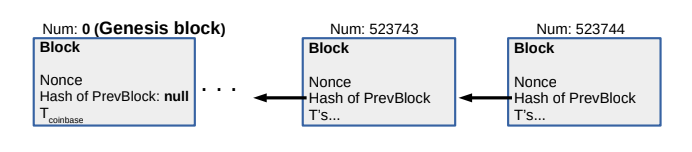
\includegraphics[width=14cm]{img/chapter_2/blocks.png}
\caption[Chaining blocks]{\footnotesize{Chaining blocks.}}
\label{fig:chaining_blocks}
\end{figure}

Mining is the process of introducing a new valid block to the network. To do so, they must perform the following steps: 
\begin{enumerate}
    \item \textbf{Transaction validation.} When a user initiates a transaction, it is broadcast to the network. Before being added to the blockchain, these transactions must be validated to ensure they adhere to the network's rules and that the sender has sufficient funds to make the transfer.
    \item \textbf{Candidate block creation.} Miners create the potential block by gathering a collection of validated transactions, known as ``mempool''. In addition, the new block must include a reference to the previous block identifier, which is a unique hash. This way we ensure a chronological order.
    \item \textbf{Proof of Work.} Before a miner can add their candidate block to the blockchain, they must solve a complex cryptographic puzzle. The operation consists of finding a \textbf{\gls{nonce}}, which will be the identifier of this new block so must be unique. This nonce has to be generated from hashing the content of the block itself and the challenge is that the hash must be led with a certain number of zeros. This property is known as \textit{``difficulty''}. Finding these hashes supposes a significant computational power.
        \begin{figure}[H]
        \centering
        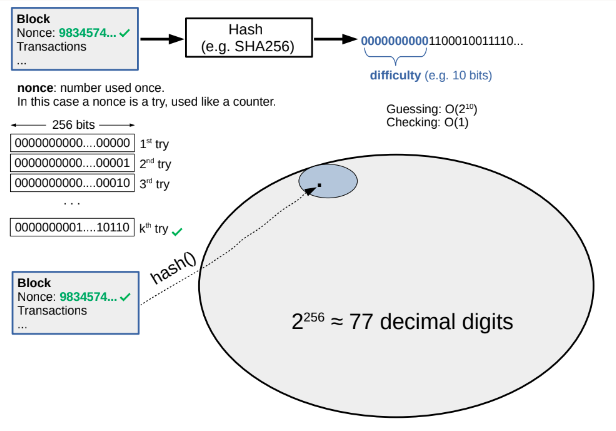
\includegraphics[width=12cm]{img/chapter_2/nonce-computation.png}
        \caption[Difficulty in nonce computation]{\footnotesize{Difficulty in nonce computation.}}
        \label{fig:Nonce-computation}
        \end{figure}
        
    \item \textbf{Competition.} Multiple miners on the network compete to solve the puzzle first like a race. Miners have to continuously calculate different nonce values until one of them successfully fits all the conditions. We can compare it to a lottery, therefore, it guarantees no single entity monopolizes the block creation.
    \item \textbf{Consensus and block addition.} Once a miner successfully solves the puzzle and adds their candidate to the blockchain it communicates the network through the ``\textit{\Gls{gossip}}". Then, other participants of the network can easily verify that the solution of your block is correct, so the consensus is reached and the new block becomes part of the blockchain.
\end{enumerate}

{To compensate the miners after accomplishing the hard task of mining there are two kinds of rewards:}
\begin{itemize}
    \item The first one is the coinbase reward. It is decided by governance consensus and it is processed at the first transaction of the block added. This is the only way of creating money in the system automatically.
    \item The second one is collecting fees from the transactions included in the block.
\end{itemize}

Nowadays, the difficulty is already to the point where it requires over a quadrillion (15 zeros) hashes to solve a block. Moreover, the probability of solving the block is fewer than one in a billion. It is also important to mention that the difficulty is adjusted to produce a constant average inter-block time (after a certain number of blocks). Inter-block time is like the \textit{blockchain clock} and allows engineering: halving date, network capacity, etc. In Bitcoin, the time inter-block is 10 minutes, whilst in Ethereum is 15 seconds, which obviously is a benefit to consider for dapps deployed in this network.

\begin{figure}[H]
\centering
\includegraphics[width=10cm]{img/chapter_2/difficulty.png}
\caption[Fixed difficulty compared to fixed time]{\footnotesize{Fixed difficulty compared to fixed time.}}
\label{fig:difficulty_comparison}
\end{figure}

History is not immediately consistent in PoW because finality is probabilistic. We have to wait to consider the blocks written in the chain immutable. For instance, Bitcoin recommends waiting 6 blocks, which is equivalent to 1 hour, to confirm a transaction.

{In a nutshell, Proof of Work consensus can be summarized with the following ideas:}
\begin{itemize}
    \item Proof of Work consists of solving a cryptographic puzzle built with a hash.
    \item Each miner is solving its own puzzle, i.e. mining its own block.
    \item Notice that the nonce is valid for a particular block only.
    \item No one needs permission to participate in the consensus and no one (banks, companies) has privileges to solve the challenge: To solve the challenge faster you need more hash power but ”anyone” can do it by buying more equipment and wasting more electricity.
\end{itemize}
}

\section{Proof of Stake}
\label{appendix:proof-of-stake}
{
{Ethereum initially was based on \acrlong{pow}, but in 2022 switched the mechanism to \acrfull{pos}\cite{proof-of-stake}. The main reasons were that it was less energy-intensive, more secure and better for implementing more scalable solutions.

In \acrlong{pos}, the participants, henceforth known as \textbf{validators}, put something valuable into the network that can be destroyed if they act dishonestly. In the case of Ethereum, validators stake capital in the form of ETH, into a smart contract on the network. The validators are in charge of checking that new blocks inserted into the network are valid and, occasionally they also create new blocks. If they behave dishonestly, for example by proposing multiple blocks instead of one or sending invalid blocks, then the consensus mechanism will destroy partially or completely their staked ETH.

Whereas under Proof of Work, the timing of blocks is determined by the difficulty as explained in the Proof of Work subsection, in Proof of Stake the timing is fixed. This time is divided into slots of 12 seconds and epochs, composed of 32 slots. Now we can evaluate how this mechanism gets a transaction executed:
}

\begin{enumerate}
    \item Users create and sign transactions, where they define the amount of gas they would pay as a \gls{tip} for validators to encourage them to include the transaction in their blocks. 
    \item The transaction is then validated by a miner, which also checks whether the sender has enough ETH to pay the transaction.
    \item Then the participant adds the transaction to his mempool of pending transactions and broadcasts the network through the \gls{gossip}, so other nodes will add it to their local mempool too.
    \item A network node is selected pseudo-randomly with the aim of proposing a block for the current slot, which will include such a transaction. This node is responsible for creating and adding the next block to the blockchain. To do so, the node runs in parallel with the execution client and the consensus client: the execution client bundles a bunch of transactions from his mempool into an \textbf{execution payload} and computes locally the new state. Such information is sent to the consensus client which wraps the payload into a \textbf{beacon block} that includes extra information about rewards, penalties, etc.
    \item Then, the nodes of the network receive the new beacon block and the execution client re-executes the transactions locally to ensure the proposed state is valid. Thereupon, the validator client attests that the block is valid and then it represents the next block of the network from its point of view. The block with the greatest weight of attestations is considered the next block of the network and the consensus is achieved.
    \item The transaction can be considered finalized whether it is part of a chain with a \textbf{supermajority link} between two checkpoints. A checkpoint is set at the beginning of an epoch and this is due to just a subset of validators attesting in each slot, whilst all validators attest during an epoch. Hence, we can only ensure the transaction is finalized between two checkpoints, a supermajority link since the 66\% of total staked ETH on the network agrees.
\end{enumerate}

{\acrlong{pos} was created to enhance the conditions of \acrlong{pow}. Staking makes it easier for individuals to participate since a validator node can run on a usual laptop and staking pools allow users to stake without having 32 ETH. Furthermore, it is more decentralized and \glspl{economy-of-scale} is much better than mining with \acrshort{pow} since it can apply economic penalties for misbehavior, making \glspl{51-attack} more costly. Moreover, it is more crypto-economic resilient. If we focus on the negative we have to mention that it is really a new player so it is not as battle-tested compared to \acrlong{pow} and it is much more complex to implement and understand because users need to run three pieces of software to participate in the mining.}

}

\section{Verify transactions with Merkle proofs}
\label{appendix:merkle-tree}
{Transactions in blockchain are verified using a cryptographic structure called \textit{Merkel tree}, also known as a binary hash tree. The Merkle tree ensures the integrity of a transaction and is really efficient to verify. To do so, the tree is constructed by hashing pairs of transactions iteratively until a single root hash is obtained. Such a node is called Merkle Root.

In the interest of verifying that a transaction is included in a block, a \textit{Merkle Proof} is generated. This proof consists of a path from the transaction's leaf node to the Merkle root, including the hash of sibling nodes along the way. As you can observe in figure \ref{fig:merkle-proof}, the root contains a contribution from all the leaves, so for \textit{n} leaves need $\log_2 n$ levels. Therefore, proofs are size $O(\log_2 n)$.

\begin{figure}[H]
\centering
\includegraphics[width=14cm]{img/chapter_2/merkle_proof.png}
\caption[Merkle proof]{\footnotesize{Merkle proof.}}
\label{fig:merkle-proof}
\end{figure}

This merely represents the way a transaction is connected to the root, so to validate the transaction we just have to hash it with the sibling hashes and following the path indicated we obtain the Merkle root. If the computed root is the same as the one coded in the block header, we can confirm the transaction is included in the block, hence it takes part in the blockchain's history.

\begin{figure}[H]
\centering
\includegraphics[width=14cm]{img/chapter_2/merkle_verification.png}
\caption[Merkle root]{\footnotesize{Merkle root in block header.}}
\label{fig:merkle-root-block-header}
\end{figure}

{Merkle proofs enhance the security and efficiency of blockchain networks by providing a way to validate transactions without the need to verify the entire block. This method ensures data integrity and allows network participants to trust the blockchain's history while conserving computational resources. It's a fundamental component of the blockchain's transparency and trustworthiness.} 
}

\section{Ethereum client}
\label{appendix:ethereum-client}
{
Ethereum is, in essence, a group of computers inter-communicated running the same software that forms a distributed network. Such computers are known as nodes, and the software they run consists of two separate clients, the execution client and the consensus client, that communicate with each other and with the network:

\begin{itemize}
    \item The execution client or Execution Engine listens to the network for new transactions. When it receives one it is executed in the EVM. Moreover, it also stores the latest state and database of all current Ethereum data.
    \item The consensus client or Beacon Node implements the \acrlong{pos} algorithm. It basically enables the node to obtain agreement based on validated data from the execution client. Furthermore, there is a third piece of software called "\textit{validator}`` that can be added to the consensus client, enabling the node capacity to participate in securing the network.
\end{itemize}


\begin{figure}[H]
\centering
\includegraphics[width=10cm]{img/ethereum/eth1eth2client.png}
\caption[Simplified diagram of how clients of a node work]{\footnotesize{Simplified diagram of how clients of a node work}}
\label{fig:node-clients}
\end{figure}

}

\section{Anatomy of smart contracts}
\label{appendix:smart-contract}
{A smart contract is basically data and functions that run on Ethereum when it receives a transaction. There are some concepts we have to consider about the data:
\begin{itemize}
    \item Modify data storage in a smart contract cost gas.
    \item There two types of data: \textbf{memory} and \textbf{storage}:
    \begin{itemize}
        \item Storage is data permanently recorded on the blockchain and needs to be typed so when it compiles the contract can keep track of how much storage it needs.
        \item Memory is where the smart contract stores the data that just lives during the contract function's execution. Since these are not permanent, they are much cheaper to use.
    \end{itemize}
    \item In addition, there are some kind of environment variables that provide data about the blockchain or current transaction, like the sender address or the block timestamp.
\end{itemize}

If we focus now on the functions, simplifying the idea they can just get information or set information in response to incoming transactions. We can divide the function calls into two types:
\begin{itemize}
    \item \textbf{Internal} functions which do not create an \acrshort{evm} call and can just be called from the current contract or derived ones.
    \item \textbf{External} functions which do create an \acrshort{evm} call and are part of the \acrshort{abi}, so they can be called from other contracts.
\end{itemize}

Another type of classification which also applies to data is:
\begin{itemize}
    \item \textbf{Public} functions which can be called internally and externally.
    \item \textbf{Private} functions which are only visible for the contract but not derived ones.
\end{itemize}

The functions of a smart contract can have different purposes:
\begin{itemize}
    \item \textbf{View functions} promise not to alter the data of the contract. For example, we can think of getter functions. 
    \item \textbf{Pure functions} promise not to either read or change data of the contract. For example, we can think about an operation function that given two integers returns the sum of them. 
    \item \textbf{Payable functions} functions that can receive ethers as input. 
    \item \textbf{Constructor functions} are only executed once at contract deployment. Typically, state variables are initialized here.
    \item \textbf{Built-in functions} that the \acrshort{evm} know how to interpret for instance \textit{address.send()} in Solidity, which is use to send \acrshort{eth} from the smart contract to that address.
    \item \textbf{Writing functions} which are the remaining can receive typed parameter variables and return typed value if desired. Moreover, it can be declared as internal/external or pure/view/payable. 
\end{itemize}
} 

\section{Evolution of the Web}
\label{appendix:web-evolution}
{The web that we use daily has been constantly evolving since it was created. The origin is defined at CERN in 1989, when Tim Berners-Lee was developing the protocols that would become the World Wide Web with the aim of creating open and decentralized protocols that allow to sharing of information from anywhere on Earth based on a \textbf{read-only model}, like a huge Wikipedia. This first approach is known as ``\textit{Web 1.0}" and the idea was maintained until roughly 2004.

With the emergence of social media platforms, the read-only model was insufficient and unable to reach such requirements. This is why the web evolved into a \textbf{read-write} model. Instead of only companies providing content to users they started to provide web applications and platforms to share user content and offer user-to-user interactions. This model supposed a revolution across the world in the sense of communication. Consequently, as more people were engaged to this platform more and more companies began to offer this kind of products and services to attract traffic and therefore, it caused the age of targeted advertising. It is important to highlight the major drawback of this ecosystem, to earn money from user content they need intermediaries, and that implies a forced trust for better or for worse. This model has been the standard until the present time.

As time went by, disruptive and very technical ideas such as blockchain appeared. This kind of technology has unlocked a lot of ideas to implement and eventually, in 2014 Ethereum proposed a solution for a problem that many early crypto adopters realized: the Web granted all the power of the data to private companies, which required too much trust. Thus, the Web is evolving again to offer a new era of a better internet. Blockchain-based, ``\textit{Web 3.0}" proposes a \textbf{read-write-own} model, where ownership gets distributed amongst content-generators and users. It is also permissionless since everyone has equal access to participate in the Web. In addition, payments and transactions occur straightforwardly without either intermediaries or opaque processes.

}

\section{Policy smart contract}
\label{appendix:policy-sc}
\begin{lstlisting}
// SPDX-License-Identifier: GPL-3.0
pragma solidity ^0.8.9;

struct Claim {
    string title;
    address expertAddress;
    uint incidentDate;
    uint expenses;
    bool approved;
    uint resolveDate;
    bool isResolved;
}


contract Policy {
    string riskData;
    uint256 premium;
    address owner;
    address public factoryAddress;
    uint endDate;
    uint renewalDate;
    uint startDate;
    mapping(uint256 => Claim) claims;
    uint256[] claimIdList;

    event Creation(address policyholderAddress);
    event Cancelation(uint endDate);
    event ClaimDeclaration(uint claimId);
    event ClaimApproved(uint claimId);
    event ClaimDeclined(uint claimId);
    event Renewal(uint endDate);

    modifier onlyFactoryOrOwner(){
        require(msg.sender == factoryAddress || msg.sender == owner, "Just the policyholder or the insurance company can perform this action");
        _;
    }

    modifier onlyOwner(){
        require(msg.sender == owner, "Just the policyholder can perform this action");
        _;
    }

    modifier onlyFactory(){
        require(msg.sender == factoryAddress, "Just the insurance company can perform this action");
        _;
    }

    modifier isActive(){
        require(endDate > block.timestamp && renewalDate > block.timestamp, "Policy is not active");
        _;
    }

    constructor(string memory _proposalData, uint256 _premium, address _owner, uint256 _endDate){
        require(_endDate > block.timestamp, "Renewal date has to be upcoming");
        require(_premium > 0 , "Required a premium to activate the policy");
        riskData = _proposalData;
        premium = _premium;
        owner = _owner;
        factoryAddress = msg.sender;
        startDate = block.timestamp;
        endDate = _endDate;
        renewalDate = _endDate;

        emit Creation(owner);
    }

    function cancelPolicy() onlyFactory() isActive external {
        endDate = block.timestamp;
        emit Cancelation(endDate);
    }

    function makeClaim(uint256 claimId, Claim memory _claim) onlyOwner isActive external {
        Claim memory newClaim = _claim;
        claims[claimId] = newClaim;
        claims[claimId].isResolved = false;
        emit ClaimDeclaration(claimId);
    }


    function approveClaim(uint256 claimId , uint256 claimExpenses) onlyFactory external {
        Claim storage claim = claims[claimId];

        resolveClaim(claimId, true);
        claim.expenses = claimExpenses;
        emit ClaimApproved(claimId);
    }

    function declineClaim(uint256 claimId) onlyFactory external{
        resolveClaim(claimId, false);
        emit ClaimDeclined(claimId);
    }

    function resolveClaim(uint256 claimId, bool isApproved) internal {
        Claim storage claim = claims[claimId];
        require(claim.isResolved == false, "Claim is already resolved");

        claim.resolveDate = block.timestamp;
        claims[claimId].isResolved = true;
        claim.approved = isApproved;

    }

    function renew(uint newEndDate) onlyFactory external returns (uint){
        require(newEndDate > endDate, "New end date has to be after the current one");
        endDate = newEndDate;
        renewalDate = newEndDate;

        emit Renewal(endDate);
        return renewalDate;
    }


    function getOwnerAddress() onlyFactoryOrOwner external view returns (address) {
        return owner;
    }

    function getClaim(uint256 claimId) onlyFactoryOrOwner external view returns (Claim memory){
        return claims[claimId];
    }

    function getClaimsList() onlyFactoryOrOwner external view returns (uint256[] memory){
        return claimIdList;
    }

    function getEndDate() onlyFactoryOrOwner external view returns (uint){
        return endDate;
    }

    function getStartDate() onlyFactoryOrOwner external view returns (uint){
        return startDate;
    }

    function getRenewalDate() onlyFactoryOrOwner external view returns (uint){
        return renewalDate;
    }

    function getRiskData() onlyFactoryOrOwner external view returns (string memory){
        return riskData;
    }

     function getPremium() onlyFactoryOrOwner external view returns (uint256){
        return premium;
    }

    function getIsActive()onlyFactoryOrOwner external view returns (bool){
        return endDate > block.timestamp;
    }

}
\end{lstlisting}

\section{Factory smart contract}
\label{appendix:factory-sc}
\begin{lstlisting}
// SPDX-License-Identifier: GPL-3.0
pragma solidity ^0.8.9;

import "./Policy.sol";


contract Factory {
    address payable public insuranceAddress;
    uint256 minimumBudget = 0.999 ether;
    mapping(address => address[]) policiesMapping;
    mapping(address => bool) private claimEvaluators;
    event PolicyCreated(address owner, uint when);
    event PolicyCanceled(address policy, uint when, uint256 amount);
    event PolicyRenewal(address policy, uint newDate, uint renewalAmount);
    event ClaimApproved(address policyAddress ,uint256 claimId , uint256 claimExpenses);
    event ClaimDeclined(address policyAddress, uint256 claimId);
    event BudgetAdded(uint amount);
    event BudgetWithdrawal(uint amount);

    constructor() payable {
        require(msg.value >= minimumBudget, "Minimum budget is not achieved to start an Insurance Smart Contract");
        insuranceAddress = payable(msg.sender);
    }


    modifier companyOnly {
        require(msg.sender == insuranceAddress, "Just the insurance company can perform this action");
        _;
    }

     modifier claimEvaluatorsOnly {
        require(msg.sender == insuranceAddress || isClaimEvaluatorKnown(msg.sender), "Required a valid evaluator approved by the company");
        _;
    }

    function addBudget() companyOnly public payable returns (uint256){
        emit BudgetAdded(msg.value);
        return address(this).balance;
    }

    function withdrawBudget(uint256 amount) companyOnly public returns (uint256){
        require(amount < address(this).balance, "There is not enough amount to withdraw");
        insuranceAddress.transfer(amount);
        emit BudgetWithdrawal(amount);
        return address(this).balance;
    }

    function createPolicy(string memory proposalData, uint endDate) public payable returns (address){
        require(msg.value > 0, "To create a policy you must pay a premium.");
        Policy policyContract = new Policy( proposalData, msg.value, msg.sender, endDate);
        address policyAddress = address(policyContract);
        address holderId = msg.sender;
        policiesMapping[holderId].push(policyAddress);

        emit PolicyCreated(msg.sender, block.timestamp);
        return policyAddress;
    }

    // Renews the policy and return the new end date.
    function renewPolicy(address policyAddress, uint newEndDate, uint renewalAmount) public payable returns (uint){
        require(msg.value > renewalAmount, "To renew a policy you must pay a premium.");
        Policy policyContract = Policy(policyAddress);
        require(msg.sender == policyContract.getOwnerAddress(), "Just the policyholder of the policy is able to renew it.");
        emit PolicyRenewal(policyAddress, newEndDate, renewalAmount);

        return policyContract.renew(newEndDate);
    }


    function approveClaim(address policyAddress ,uint256 claimId , uint256 claimExpenses) claimEvaluatorsOnly public {
        require(claimExpenses < address(this).balance, "Insufficient balance to pay the claim.");

        Policy policy = Policy(policyAddress);
        policy.approveClaim(claimId, claimExpenses);

        address payable holderAddress = payable(policy.getOwnerAddress());
        emit ClaimApproved( policyAddress, claimId, claimExpenses);
        holderAddress.transfer(claimExpenses);
    }

    function declineClaim(address policyAddress, uint256 claimId) claimEvaluatorsOnly public {
        Policy policy = Policy(policyAddress);
        emit ClaimDeclined(policyAddress, claimId);
        policy.declineClaim(claimId);
    }

    function addEvaluator(address newAddress) companyOnly public {
        claimEvaluators[newAddress] = true;
    }

    function changeEvaluatorValue(address evaluator, bool value) companyOnly public {
        claimEvaluators[evaluator] = value;
    }

    function isClaimEvaluatorKnown(address checkAddress) companyOnly public view returns(bool) {
        return claimEvaluators[checkAddress];
    }

    function getHolderPolicies() public view returns (address[] memory){
        return policiesMapping[msg.sender];
    }

    function cancelPolicy(address addressPolicy)  public {
        Policy policy = Policy(addressPolicy);
        address owner = policy.getOwnerAddress();

        require(msg.sender == owner || msg.sender == insuranceAddress, "Just the policyholder of the policy is able to cancel it.");
        policy.cancelPolicy();

        uint premium = policy.getPremium();
        uint256 startDate = policy.getStartDate();
        uint256 renewalDate = policy.getRenewalDate();
        uint256 cancellationDate = policy.getEndDate();

        uint256 timeNotEnjoyed = renewalDate - cancellationDate;
        uint256 totalTimeSpan = renewalDate - startDate;

        uint256 timePercentage = (timeNotEnjoyed * 100) / totalTimeSpan;
        address payable holderAddress = payable(owner);
        uint256 amountToReturn = premium * timePercentage / 100;

        require (amountToReturn < address(this).balance, "Insufficient balance to pay the cancellation.");

        holderAddress.transfer(amountToReturn);
        emit PolicyCanceled(addressPolicy, cancellationDate, amountToReturn);
    }
}


\end{lstlisting}


\end{appendices}

\end{document}
